\documentclass[11pt]{article}
\usepackage{ctex}

\usepackage[left=1.25in,right=1.25in,top=1in,bottom=1in]{geometry}
\usepackage{graphicx}
\usepackage{float}
\usepackage{extarrows}
\graphicspath{{figures/}}

\usepackage{fontspec}
\usepackage{amsthm,amsmath,amssymb,mathrsfs}

\begin{document}
	\title{Some imformation about article}
	
	\maketitle
	
	\newpage
	\tableofcontents
	\newpage

\section{Simple Baselines for Human Estimation and Tracking}
$\text{https://github.com/Microsoft/human-pose-estimation.pytorch}$
\subsection{Introduction}

Algorithm and system complexity increase.The paper provides simple and effective baseline methods.Many vision tasks are significantly advanced by deep learning.

There are two state-of-the-art network architectures for pose estimation:
1.one stage in Hourglass.
2.CPN(Cascaded Pyramid Network)

The main task of pose estimation is 'how high resolution feature maps are generated'.In other words 'Obtaining high resolution feature maps is crucial,but no matter how.

The steps of Multi-person pose tracking in videos:
1.estimate human poses in frames.
2.track these human pose by assigning a unique ID to them across frames.

Pose tracking is the task of estimating multi-person human poses in videos and assigning unique instance IDs for each keypoint across frames.

We will expand the box where propagate joint location 15\% in experiments.We could have boxes propagated from previous frames where people have been detected correctly.We can track result in previous frames.


\subsubsection{The past reasult in some dataset}

MPII benchmark starte from about 80\% PCKH@0.5 to more than 90\%.The leading methods on MPII benchmark have considered many details in different wats but minor difference in accuracy.

COCO human pose benchmark is even faster, the mAP metric is increased from 60.5 to 72.1

\subsection{Network}

Resnet is the most common backbone network for image feature extraction.Resnet is the simplest way to estimate heat maps from deep and low resolution feature maps.(mAP of 73.7 on COCO testdev split)

The network of this paper is a backbone network(ResNet) with a few deconvolutional layers(C5).C5 uses the batch normalization and Relu activation.We adopt this structure because it is arguably the simplest to generate heatmaps from deep and low resolution features and also adopted in the Mask R-CNN

The Greedy matching algorithm is about how to repeat the ID or assign a new ID number.(Mask RCNN and greedy bipartite matching algorithm)

\begin{figure}[h]
	\centering
	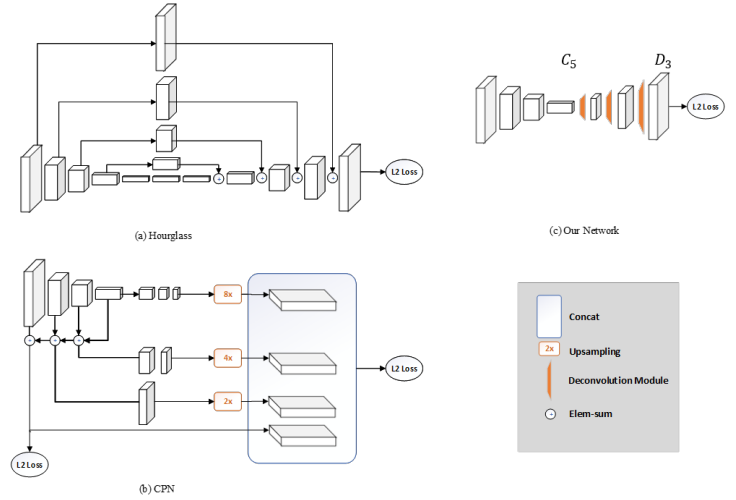
\includegraphics[scale = 0.5]{1}
\end{figure}

Mean Squared Error(MSE) is used as the loss between the presicted heatmaps and targeted heatmaps.

Some detector for single image level or maybe videos (Faster-RCNN,R-FCN)

The flow-based inference algorithm for video human pose tracking

The first problem is pose estimation problem(mainly use a bounding box Non-Maximum Suppression(NMS))
The second problem is tracking problem(mainly the Q used to capture previous multi frames' linking relationship,the Q's length indicates how many previous frames considered when performing matching)

INPUT:

video frames(A), Q = [](Q's max capacity LQ)

Process:

1.person detection network to get person (B)

2.meantime video frame(B)and frame that get person(A) get into human pose estimation network can get the first frame(C)

3.initialize the id for the first frame(C)

4.append id and the first frame(C) into Q

5.get into the loop to deal with video frames after the first frame

LOOP(k = 1 to inf):

1.person detection network to get person

2.put the before human pose estimation network's reasult(k-1) and flow field frame k-1 to frame k to generate boxes by joint propagating

3.use NMS(Non-Maximum Suppression) to unify detection boxes and flow boxes

4.use NMS'result and the k frame into human pose estimation network to get(J)

5.put G and Q to get into funtion for similarity matrix to get similarily matrix(M)

6.put M and J into function for assigning instance id to get the frame unique id(P)

7.append the P to the Q(update the Q)

\begin{figure}[h]
	\centering
	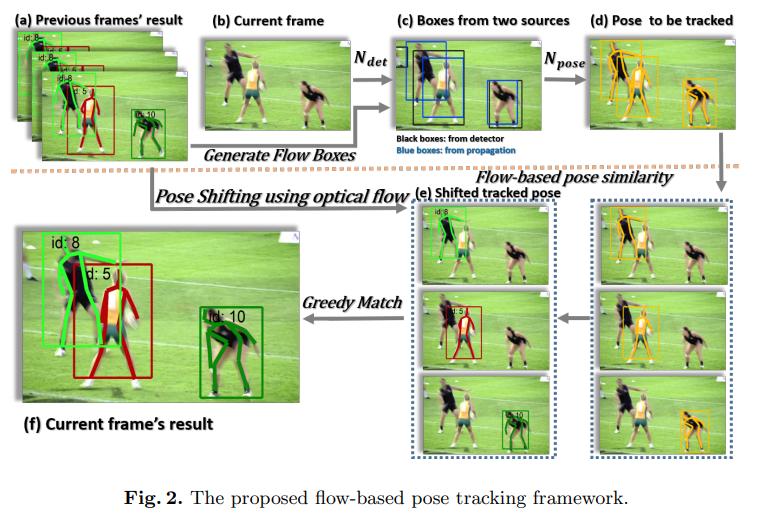
\includegraphics[scale = 0.5]{2}
\end{figure}

\subsection{Conclusions and Contributions}

We present simple and strong baseline for pose estimation and tracking.The contribution of the work are soild baselines for the field(in other words,after this paper the results of other reaserch must do better than the reasult in this paper)

1.Two different kind of human boxes(one is a human detector, other is boxes generated from previous frames using optical flow)

2.Using a metric similar with greedy matching algorithm
\subsection{Ablation Study}
Table \ref{tab1} investigates various options in our baseline.
\begin{figure}[H]
	\centering
	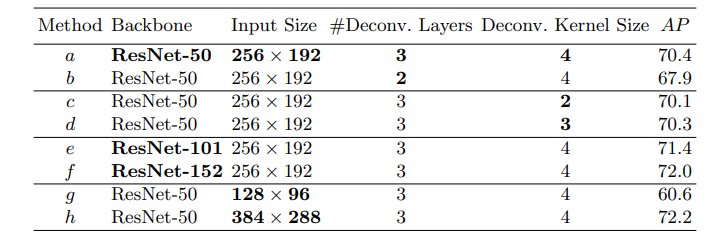
\includegraphics[scale = 0.7]{24}
	\caption{Ablation study of our method on COCO val2017 dataset}
	\label{tab1}
\end{figure}

Comparing our results with a 8-stage Hourglass and CPN on COCO val2017 dataset.OHKM means Online Hard Keypoints Mining.
\begin{figure}[H]
	\centering
	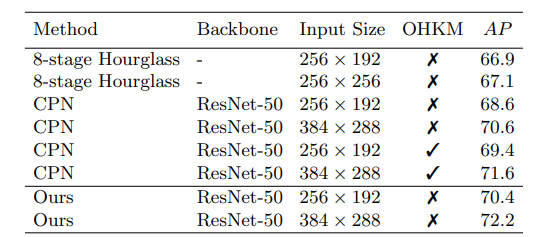
\includegraphics[scale = 0.7]{25}
\end{figure}

Comparisons on COCO test-dev dataset.
\begin{figure}[h]
	\centering
	
\includegraphics[scale = 0.5]{26}
\end{figure}
\subsection{The direction after this paper}

"Simultaneous pose dectation and tracking in wild" or the pose tracking(Using the greedy matching method) 
\section{LightTrack: A Generic Framework for Online Top-Down Human Pose Tracking}
$\text{https://github.com/Guanghan/lighttrack}$
\subsection{Abstract}
The proposed framework is designed to be generic for top-down pose tracking and is faster than existing online and offline methods.

Single-person Pose Tracking(SPT) and Visual Object Tracking(VOT) are incorporated into one unified functioning entity,replaced single-person pose estimation module.

Our framework unifies single-person pose tracking with multi-person identity association.Bridging keypoint tracking with object tracking.

Siamese Graph Convolution Network(SGCN) for human pose matching as a Re-ID module(using a graphical representation of human joints for matching ) in our pose tracking system.

The skeletonbased representation effectively captures human pose similarity and is computationally inexpensive.

It is robust to sudden camera shift that introduces human drifting.

To the best of our knowledge, this is the first paper to propose an online human pose tracking framework in a top-down fashion.

The proposed framework is general enough to fit other pose estimators and candidate matching mechanisms.

Our method outputforms other online methods while maintaining a much higher frame rate, and is very competitive with our offline state-of-the-art.
\subsection{Introduction}
Accurate estimation of human keypoint-trajectories is useful for human action recognition, human interaction understanding, motion capture and animation.

More emphasis has been put on the Multi-Object Tracking Accuracy(MOTA) criterion compared to the Frame Per Second(FPS) criterion.

In this paper,we propose anovel effective light-weight framework for pose tracking.

We track each human pose by recursively updating the bounding box and its corresponding pose in an explicit manner.

The bounding box region of a target is inferred from the explicit features(the human keypoints)

The advantages of using pose as explicit features include:

(1).The explicit features have very strong and stable relationship with the bounding box position.

(2).Tracking requires human keypoints,taking advantage of the predicted keypoints is efficient in tracking the ROI region.

(3).Most exising methods are offline hence lacking the potential to be real-time.
\subsection{Related Work}
\subsubsection{Human Pose Estimation and Tracking(HPE)}

Multi-person human pose estimation is more realistic and challenging.

Existing methods can be classified into top-down and bottom-up approaches.

The top-down approaches rely on the detection module to obtain human candidates and then applying single-person pose estimation to locate human keypoints.

The advantage of top-down approaches is their capability in disassembling the task into multiple comparatively easier tasks(object detection and single-person pose estimation) 

The bottom-up methods detect human keypoints from all potential candidates and then assemble these keypoints into human limbs for each individual based on various data association techniques.

The advantage of bottom-up approaches is thire excellent trade-off between estimation accuracy and computational cost because the cost is nearly invariant to the number of human candidate in the image.

The task is to estimate human keypoints and assign unique IDs to each keypoint at
instance-level across frames in videos.
\subsubsection{Object Detection vc. Human Pose Estimation}
Earlier works in object detection regress visual features into bounding box coordinates.

These works predict heatmaps for a set of special keypoints to infer detection results (bounding boxes).

\subsubsection{Multi-Object Tracking}
MOT aims to estimate trajectories of multiple objects by finding target locations while maintaining their identities across frames.

Offline methods use both past and feature frames to generate trajectories.Online methods only exploit information that is available until the current frame.

Our proposed online pose tracking framework also tracks each target (with corresponding keypoints) individually while keeping their identities, and performs data association when target is lost.

However, our framework is distinct in several aspects: 

\noindent (a) the detection is generated by object detector only at key frames, therefore not necessarily provided at each frame. It can be provided scarcely;

\noindent (b) the single object tracker is actually a pose estimator that predicts keypoints based on an enlarged region.
\subsubsection{Graphical Representation for Human Pose}
It is recently studied on how to effectively model dynamic skeletons with a specially tailored graph convolution opertion.

The graph convolution operation turns human skeletons into spatio-temporal representation of human actions.

We propose to employ GCN to encode spatial relationship among human joints into a latent representation of human pose. The representation aims to robustly encode the pose, which is invariant to human location or view angle.

We measure similarities of such encodings for the matching of human poses.
\subsection{Method}
\subsubsection{Top-Down Pose Tracking Framework}
It has been proved that human pose can be employed for better inference of human locations.

We observe that accurate human locations also ease the estimation of human poses in a top-down approach.

Some relation-ships between these two levels of information:

\noindent 1.Coarse person location can be distilled into body keypoints by a single-person pose estimator.

\noindent 2.The position of human joints can be straightforwardly used to indicate rough locations of human candidates.

\noindent 3.Recurrently estimating one from the other is a feasible strategy for Single-person Pose Tracking(SPT).

For the  Multi-target Pose Tracking(MPT) problem,a better way is to track multiple individuals simultaneously and preserve/update their identities with an additional Re-ID module.

The Re-ID module is essential because it is usually hard to maintain correct identities all the way.

For instance, under the following scenarios,identities have to be updated:

\noindent (1) some people disappear from the camera view or get occluded;

\noindent (2) new candidates come in or previous candidates re-appear;

\noindent (3) people walk across each other (two identities may merge into one if not
treated carefully);

\noindent (4) tracking fails due to fast camera shifting or zooming.

\textbf{Our Method}:

We first treat each human candidate separately such that their corresponding identity is kept across the frames(We circumvent the time-consuming offline optimization procedure)

If we lost tracked candidate, we then call the detection module to revive candidates and associate them to the tracked targets from the previous frame via pose matching.

So we accomplish multi-target posr tracking with an SPT module and a pose matching module.

the bounding box of the person in the upcoming frame is inferred from the joints estimated by the pose module from the current frame. We find the minimum and maximum coordinates and enlarge this ROI region by 20\% on each sideThe enlarged bounding box is treated as the localized region for this person in the next frame.

If the average confidence score from the estimated joints is lower than the standard, it reflects that the target is lost.

If the target is lost two modes:

\noindent 1.Fixed Keyframe Interval(FKI) mode: Neglect this target until
the scheduled next key-frame, where the detection module re-generate the candidates and then associate their IDs to the tracking history.(The advantage of FKI mode is that the frame rate of pose tracking is stable due to the fixed interval of keyframes)

\noindent 2.Adaptive Keyframe Interval (AKI)mode: Immediately revive the missing target by candidate detection and identity association.(The advantage of AKI mode is that the average frame rate can be higher for noncomplex videos)

In our experiments, we incorporate them by taking keyframes with fixed intervals while also calling detection module once a target is lost before the arrival of the next arranged keyframe.

For identity associationwe propose to consider two complementary information: spatial consistency and pose consistency.

\noindent Spatial Consistency:

if two bounding boxes from the current and the previous frames are adjacent, or their Intersection Over Union (IOU) is above a certain threshold, we consider them to belong to the same target.

$$m(t_k,d_k) = \left\{\begin{matrix}
	1,& \qquad if o(t_k,D_{i,k})> \tau_o\\ 
	0,& \qquad otherwise
\end{matrix}\right.$$

The above criterion is based on the assumption that the tracked target from the previous frame and the actual location of the target in the current frame have significant overlap, which is true for most cases.

When the camera shiftly, we need to match the new observation to the tracked candidates.

Some drawback about other Re-ID mathods: 1.Visually similar candidates with different identities may confuse such classifiers. 2.Extracting visual features can also be computationally expensive in an online tracking system.

We observe that in two adjacent frames, the location of a person may drift away due to sudden camera shift, but the human pose will stay almost the same as people usually cannot act that fast.

Consequently, the graph representation of human skeletons can be a strong cue for candidate matching, which we refer to as pose matching in the following text.
\subsubsection{Siamese Graph Convolutional Networks}
\textbf{Siamese Network:}

The input to our graph convolutional network is the joint coordinate vectors on the
graph nodes. It is analogous to image-based CNNs where the input is formed by pixel intensity vectors residing on the 2D image grid.

Multiple graph convolutions are performed on the input to generate a feature representation
vector as a conceptual summary of the human pose. It inherently encodes the spatial relationship among the human joints. 

The input to the siamese networks is therefore a pair of inputs to the GCN network. The distance between two output features represent how similar two poses are to each other.
\begin{figure}[H]
	\centering
	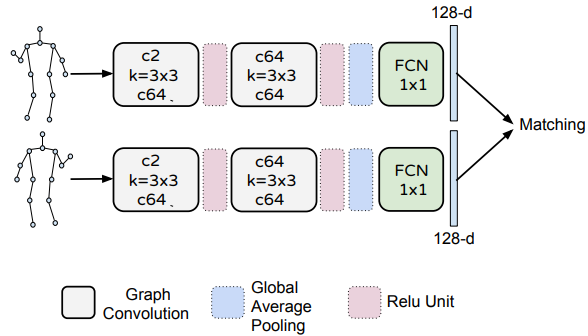
\includegraphics[scale = 0.6]{27}
\end{figure}
We extract two feature vectors from the input graph pair with shared network weight. The feature vectors inherently encode the spatial relationship among the human joints.

\textbf{Graph Convolution for Skeleton:}
$$f_{out}(v_i) = \sum_{v_j\in B(v_i)}\frac{1}{Z_i(v_j)}f_{in}(p(v_i,v_j))\dots w(v_i,v_j)$$
where the normalization term $Z_i(v_j) = {v_k|l_i(v_k) = l_i(v_j)}$ is to balance the contributions of different subsets to the output.

$$l_i(v_j) = \left\{\begin{matrix}
	0& \qquad if\quad r_j=r_i\\ 
	1& \qquad if\quad r_j<r_i\\
	2& \qquad if\quad r_j>r_i 
\end{matrix}\right.$$

where $r_i$ is the average distance from gravity center to joint i over all frames in the training set.
\begin{figure}[H]
	\centering
	
\includegraphics[scale = 0.6]{28}
\end{figure}
The nodes are labeled according to their distances to the skeleton gravity center (black circle) compared with that of the root node (green). Centripetal nodes have shorter distances (blue), while centrifugal nodes have longer distances (yellow) than the root node.



\subsection{Conclutions and Contributions}

Our method outperforms other online methods while maintaining a higher frame rate, and is very competitive with our offline state-of-the-art

The proposed framework is general enough to fit other pose estimators and candidate matching mechanisms.

\section{PoseTrack A Benchmark for Human Pose Estimation and Tracking}


\subsection{Abstract}

Exising systems for video-based pose estimation and tracking struggle to perform well on realistic videos with multiple people and often fail to output body-pose trajectories consistent over time.

To address this shortcoming this paper introduces PoseTrack which is a new large-scale benchmark for video-based human pose estimation and articulated tracking.

Our new benchmark encompasses three tasks focusing on i)single-frame multi-person pose estimation, ii)multi-person pose estimation in videos, iii)multi-person articulated tracking.

new dataset,LSP,LSP Extended,MPII Human Pose(Single Person),MS COCO Keypoint Challenge,else in table 1.

\subsection{Introduction}

Importantly, these benchmark datasets not only have provided extensive training sts required for training of deep learning based approaches, but also established detailed metrics for direct and fair performance comparison across numerous competing approaches.

Significant progress of single frame based multiperson pose estimation.It's still problem about articulated multiperson body joint tracking in monocular video.

In the work,we aim to fill this gap by establishing a new large-scale, high-quality benchmark for video-based multi-person pose estimation and articulated tracking. 

Three related tasks focuse on 1.single-frame multi-person pose estimation,2.multi-person pose estimation in video,3.multi-person articulated tracking.

\subsection{Data Annotation}
\begin{figure}[H]
	\centering
	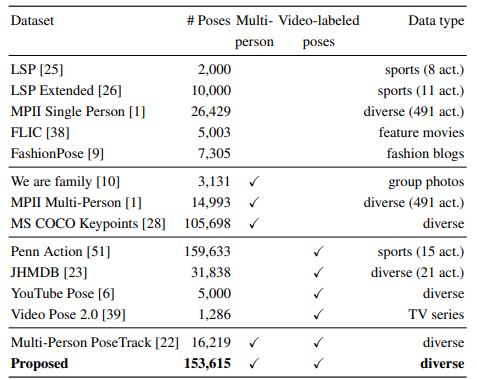
\includegraphics[scale = 0.6]{29}
	\end{figure}
We annotated the selected video sequences with person locations, identities, body pose and ignore regions.

The annotations are about four steps:
1.we labele ignore regions to exclude crowds and people for which pose can not be relibly determined due to poor visibility.
2.the head bounding boxes for each person across the videos are annotated and a track ID is assigned to each person.
3.assign a unique track ID to each person appearing in the video until the person moves out of the camera field-of-view
4.maintain track ID between shots and same person might get different track ID if it reappears in another shot

Annotation strategy:for each sequence in our benchmark we annotate the 30 frames in the middle of the sequence.In addition, we annotate validation and test sequences with a step of four frames.(aim to evaluate both smoothness of body joint tracks as well as ability to track body joints over longer number of frames)

\subsection{Challenges}

The benchmark consists of the following challenges:

Single-frame pose estimation:this task is similar to the ones covered by existing datasets like MPII Pose and MSCOCO Keypoints.

Pose estimation in videos:the evaluation of this challenge is performed on single frames,but the data will also include video frames before and after the annotated ones.

Pose tracking:this task requires to provide temporally consistent poses for all people visible in the videos.
\subsection{Experimental Setup}

In order to evaluate whether a body part is predicted correctly, we use the PCKh(head-normalized probability of correct keypoint) metric, which considers a body joint to be correctly localized if the predicted location of the joint is within a certain threshold from the true location.

Due to large scale variation of people across videos and even within a frame, this threshold needs to be selected adaptively based on the person's size

Two sets of evaluation metrics:one use for evalusting multi-person pose estimation,one from the multi-target tracking literature to evaluate multi-person pose tracking.

We ignore all person detections that overlap with the ignore regions.

Multi-person pose estimation:we use mean Average Precision(mAP) to measure frame-wise multi-person pose accuracy.(way:we propose not to use any ground-truth information during testing and evaluate the predictions without rescaling or selecting a specific group of perple for evaluation)

Evaluate multi-person pose estimation requires that the location of a group od persons and their rough scale is known during evaluation,but this information is never available in realistic scenarios,particularly for videos.

Articulated multi-person pose tracking:we use MOT(Multiple Object Tracking)metrics and  apple them independently to each of the body joints

The way to get MOT metrics(require predicted body poses with track IDs):1.Compute distances between predicted and ground-truth locations for each frame, for each body joint class. 2.Match predicted and ground-truth locations by a global matching procedure that minimizes the total assignment distance. 3.Compute MOTA(Multiple Object Tracker Accuracy),MOTP(Multiple Object Tracker Precision),Precision and Recall metrics


\subsection{The State of Art}

Articulated pose tracking in unconstrained videos is a relatively new topic in compuer vision research.

We processed in two ways to analyze the performance of the state of the art on our new dataset.

First, we propose two baseline methods based on the state-of-the-art approaches.We modify these methods to make them applicable on our proposed dataset.

Second,in order to broaden the scope of our evaluation we organized PoseTrack Challenge in conjunction with ICCV'17 our dataset by establishing an online evaluation server and inviting submissions from the research community.

\section{Pose Recognition with Cascade Transformers}
$\text{https://github.com/mlpc-ucsd/PRTR}$
\subsection{Abstract}

We present a regression-based pose recognition method using cascade Transformers.We utilize the encoder-decoder structure in the Transformers to perform regression-based person and keypoint detection that is general-purpose and requires less heuristic design compared with the existing approaches.

One way to categorize the existing approaches in this domain is to separate them into 1.heatmap-based 2.regression-based.

Heatmap-based methods can achieve higher accuracy but are subject to various heuristic desighs(not end-to-end mostly).

Regression-based methods have less intermediate non-differentiable steps but lower accuracy.

We demonstrate the keypoint hypothesis(query) refinement process across different self-attention layers to reveal the recursive self-attention mechanism in Transformers. 

\subsection{Introduction}

Pose recognition is a challenging problem that remains unsolved.The difficulty lies in various aspects such as large pose/shape variation,inter-person and self occlusion,large appearance variation,and background clutter.

The task of pose recognition is to localize the human keypoint(17 in the experiments) for the individual persons in two ways.

1.Top-down process:persons are detected first,followed by keypoint detection from the detected image region/patch.

2.Bottom-up process:human keypoints are detected directly from the image without an explicit object detection stage.

3.Heatmap or Regression:heatmap-based methods are adopted when the accuracy is the priority whereas regression-based approaches can be considered as a convenient plug-and-play module.

Heatmap approaches perform dense keypoint detection followed by subsequent processes for clustering and grouping;they deliver strong performance but are also subject to many heuristic designs that are mostly not end-to-end learnable.

Regression perform regression for the keypoints directly which have less intermediate stages and specifications.

DARK presents Taylor-expansion based coordinate decoding and unbiased sub-pixel centered coordinate encoding.

UDP even discovered a considerable accuracy decrease when using one-pixel flip shift in heatmap-based paradigms.

For general-purpose regression methods, we aim at removing unnecessary designs by making the training objective and target output direct and transparent.Coordinates should be output direct and loss be calculated with predictions and ground truth coordinates straightforward.

We present a top-down regression-based 2D human pose recognition method using cascade Transformers consisting of a person detection Transformer and a keypoint detection Transformer.

Two alternatives in Pose Recognition with TRansformer(PRTR):1.a two-stage process 2.a sequential process with the two transformers(end-to-end).

We apply multi-scale features in the keypoint detection Transformer.

\subsection{Contributions}

1.We propose a regression-based human pose recognition method(PRTR) by buliding cascade Transformers,based on a general-purpose object detector,end-to-end object detection Transformer(DETR).

Tokenized representation in Transformers with layers of self-attention to capture the joint spatial and appearance modeling for the keypoints.

2.Two types of descade Transformers:1.two-stage process;2.sequential use spatial Transformer network(STN)

3.We visualize the distribution of keypoint queries in various aspects to unfold the internal process of the Transformer for the gradual refinement of日 the detection.

As far as we know, we are the first to visualize the dynamic decoding process in Transformer decoder, which brings significant insights to future Transformer designs.But there are limited visualization works compared with those done on language application.
\subsection{Related Work}

HRNet family model(advance for 2D human pose recogniton/estimation) is itself about a new convolutional neural network(CNN) architecture targeting the modeling of high-resolution feature reponses.

Heatmap-based:the classifiers produce dense heatmaps(classification map),followed by clustering and grouping processes.

On one hand,leveraging fine-grained detection for keypoints by densely scanning all the pixels.On the other hand,heatmaps create a disconnection from the overall estimation of the keypoints,making the intermediate clustering and grouping process not directly integrable to be end-to-end learning frameworks

Regression-based:aiming to direactly approach keypoint detection with a direct loss minimization between predicted and ground truth coordinates.They can be more easily integrated into an end-to-end learning framework.It skips a large number of candidate locations,creating a performance gap with the heatmap-basd methods.

Transformers and self-attention:The introduction od Transformers to object detection gives another leap-forward in building end-to-end object detection framework that is free of proposal,anchor and post processing(non-maximum suppression)

\subsection{Method}

Illustration of the gradual refinement for the keypoints across different Transformer decoder layers.Through the decoding process, PRTR predicts keypoints with increasing confidence and decreasing spatial deviation to ground truth,transforming image-ignorant queries to final predictions.
\begin{figure}[H]
	\centering
	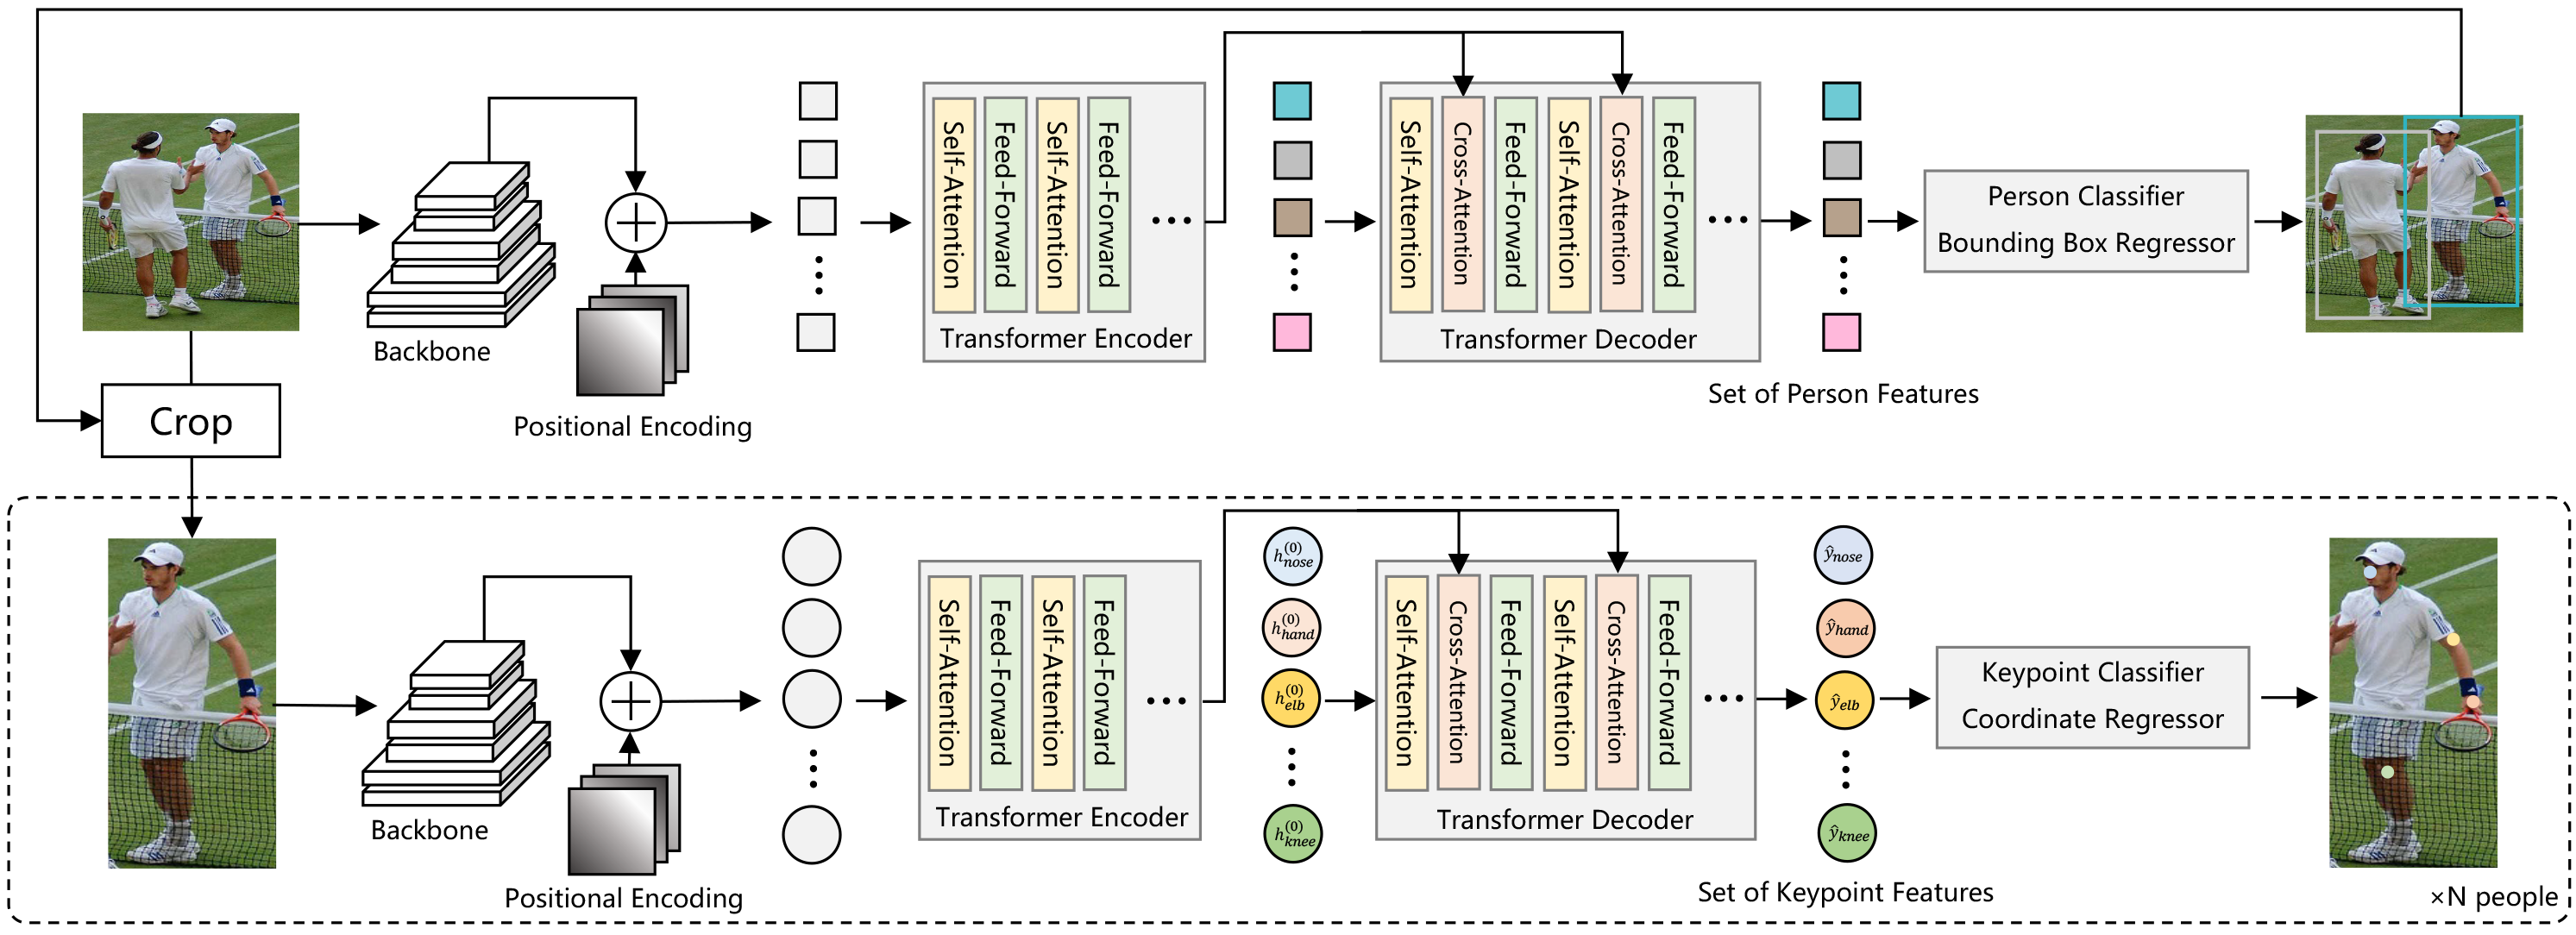
\includegraphics[scale = 0.6]{30}
	\caption{model two stage}
\end{figure}
\begin{figure}[H]
	\centering
	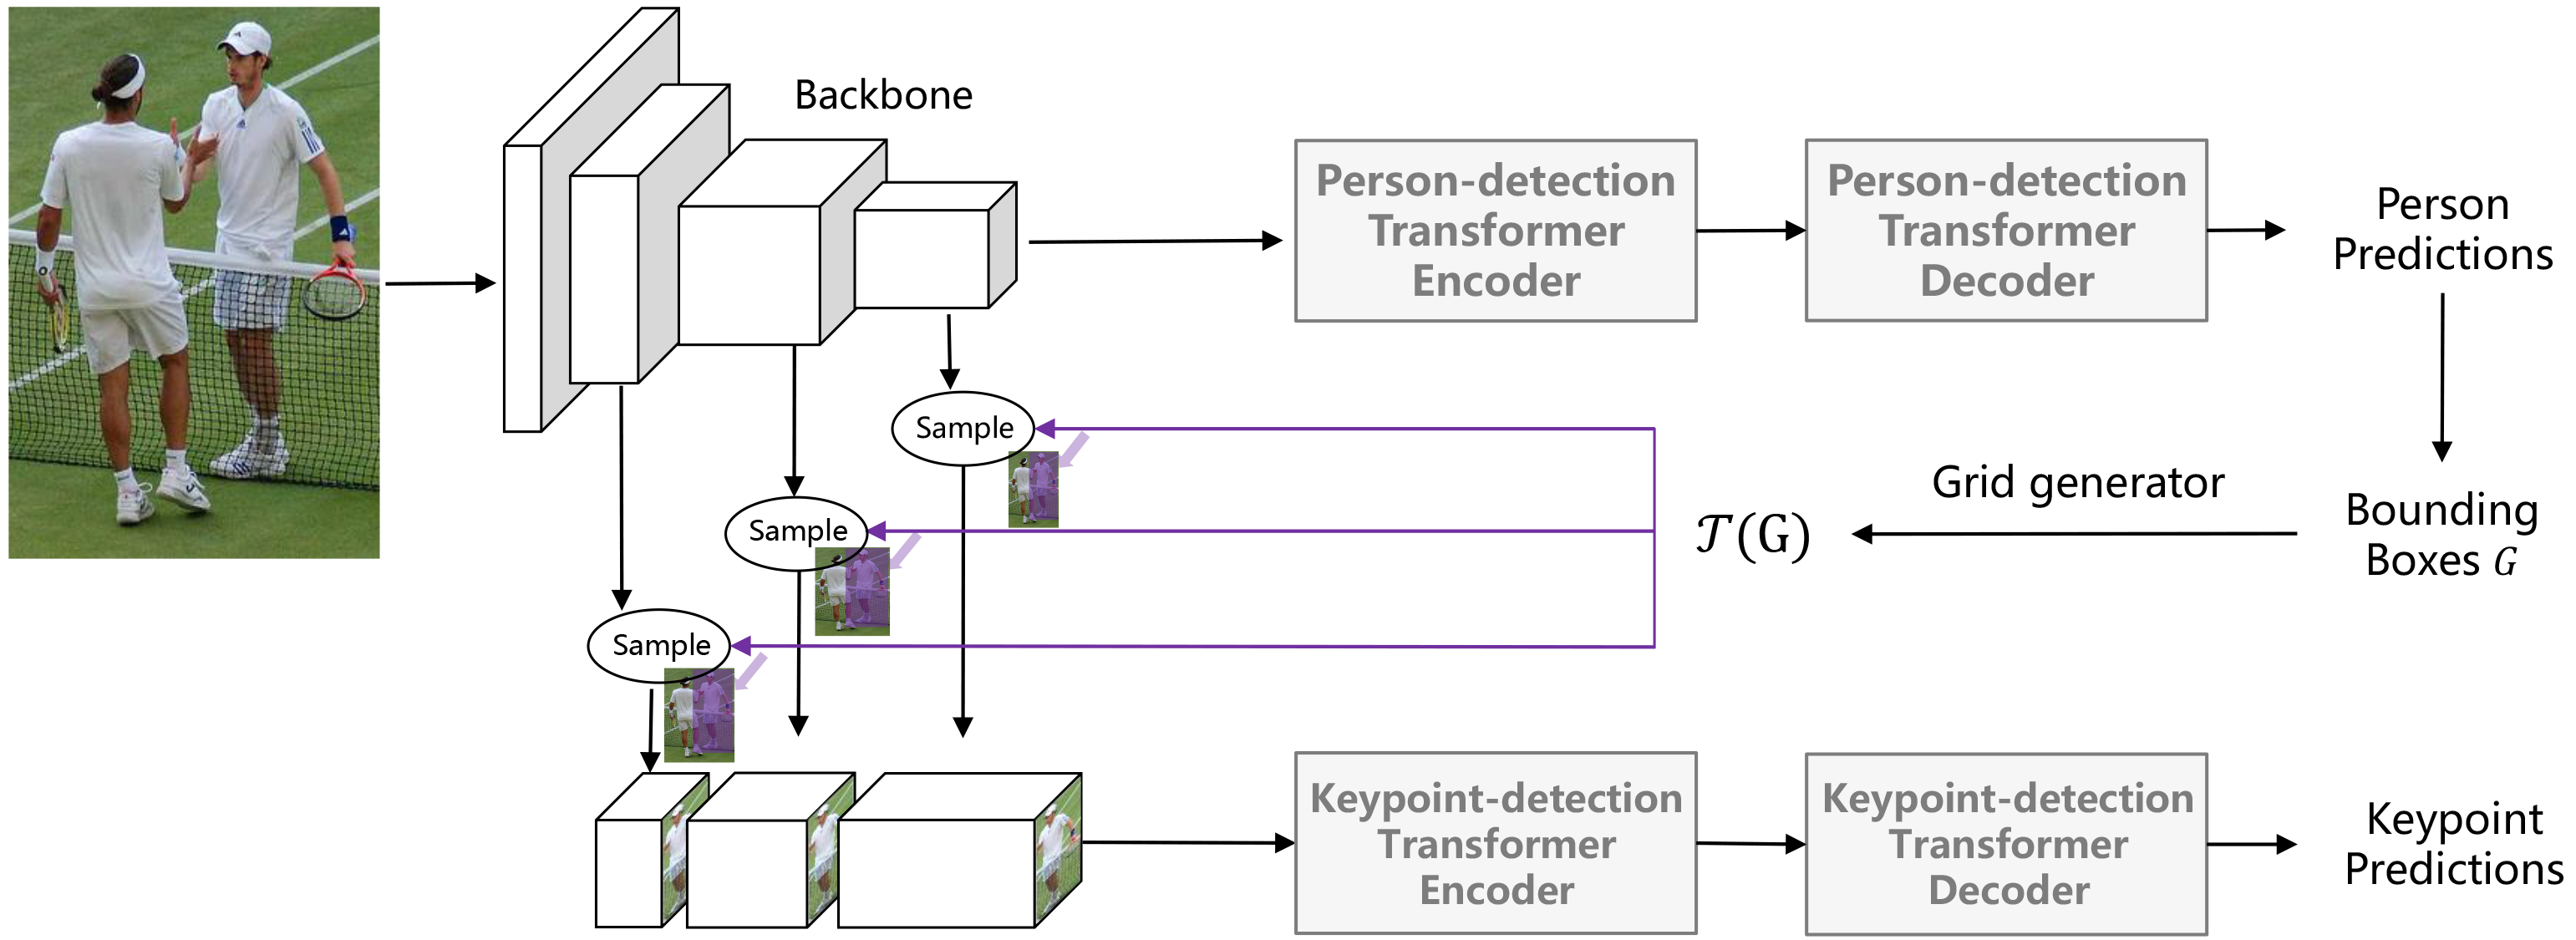
\includegraphics[scale = 0.6]{31}
	\caption{model sequential}
\end{figure}
\subsubsection{Person-Detection Transformer}

We trakle nulti-person pose recognition problem in a top-down manner.

The first-stage person detection backbone: Transformer architecture following DEtection TRansformer(DETR).

The encoder stage:image features generated by a CNN are flattened and fed into a Transformer encoder to produce contextualized image features.

The decoder stage:given a fixed set of learned query embedding as input, Transformer decoder reasons about the relations between object queries in a parallel way.

At last, a classification head is used to classify the object as person or background and a 4-channel regression head is used to predict the bounding boxes.

\subsubsection{Keypoint-Detection Transformer}

After getting the bounding boxes,we crop the RGB image and use another CNN backbone to get feature maps per person.

Because only matched queries are involved in calculating the loss for keypoint-detection Transformer, we filtered out unmatched ones.

We use the encoder-decoder architecture of the Transformer to predict in a parallel fashion,but we use another set of queries(quantity denoted Q)

Finally,a classification head predicts among J types of joints and background($\emptyset$) and 2-channel regression head outputs the coordinate of each keypoint.

PRTR infers a fixed larger number(Q) of predictions than ground truth(J),we need to find a matching between them to calculate the loss.

We formulate this matching problem as an optimal bipartite matching problem,which can be solved efficiently by Hungarian algorithm.

At training stage,we match our queries using a mixture of classification probabilities and coordinate deviation.

At inference stage,we do not have access to the ground-truth keypoint coordinates, thus we match J prototype keypoints to querues using only the classification probabilities.

For matched queries, we calculate the loss function.For unmatched queries we only backpropagate the classification loss.To address the class imbalance caused by $\emptyset$ class, we set the weight of its log-probability term to 0.1.

\subsubsection{Multi-layer Cropping with STN}

Under an end-to-end philosophy,it is desired that the model is end-to-end tunable to exploit the synergy between person detection and keypoint recognition task.

We incorporate the Spatial Transformer Network(STN) to crop out image features needed by the keypoint-detection Transformer directly from the feature map generated by the first CNN backbone.

This cropping operation is differentiable not only to the feature maps,but also to the bounding box coordinates.

We apple the grid to feature maps of different scales generated at different intermediate layers of the CNN backbone using a bilinear kernel to mitigate the resolution challenge commonly seen in keypoint recognition.(differentiable bilinear sampling)

After getting a series of image features of the same spatial size, we concatenate them into a single feature map for the keypoint-detection Transformer.
\subsection{Experiment}
We validate our proposed method on the COCO Keypoint Detection task and MPII Human Pose Dataset.
\begin{figure}[H]
	\centering
	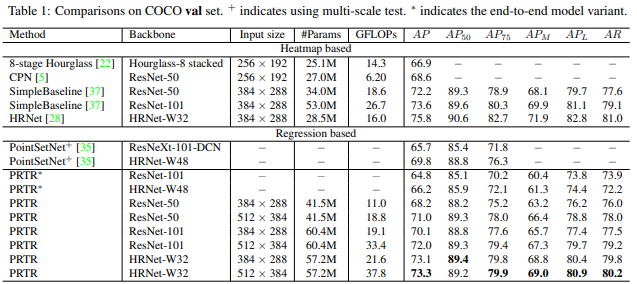
\includegraphics[scale = 0.6]{32}
\end{figure}

Comparisons on COCO test-dev set.
\begin{figure}[H]
	\centering
	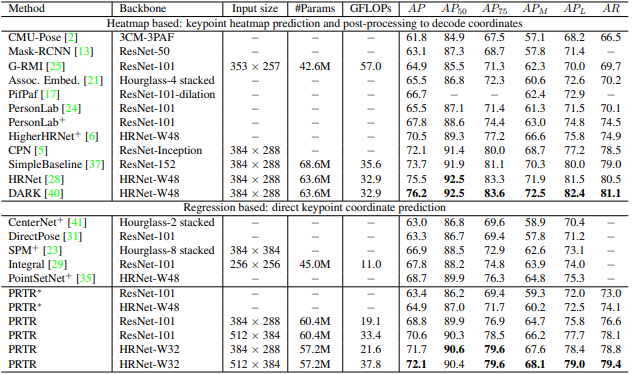
\includegraphics[scale = 0.6]{33}
\end{figure}

\begin{figure}[H]
	\centering
	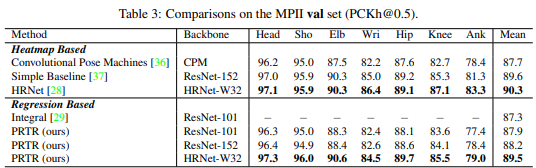
\includegraphics[scale = 0.6]{34}
\end{figure}

Ablation study on COCO val2017.'GT Box'represent ground truth box for cropping,'$\text{\o}$ Logit'and inclusion of background logits during inference respectively.
\begin{figure}[H]
	\centering
	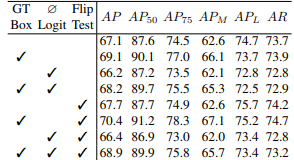
\includegraphics[scale = 0.6]{35}
\end{figure}
\section{Bottom-Up Human Pose Estimation Via Disentangled Keypoint Regression}
$\text{https://github.com/HRNet/DEKR}$
\subsection{Abstract}
We study the dense keypoint regression framework that is previously inferior to the keypoint detection and grouping framework. 

Our motivation is that regressing keypoint positions accurately needs to learn representations that focus on the keypoint regions.Our mathods are keypoint detection and grouping methods.

We present a simple yet effective approach, named disentangled keypoint regression(DEKR).

We adopt adaptive convolutions through pixel-wise spatial transformer to activate the pixels in the keypoint regions and accordingly learn representations from them.We use a multi-branch structure for separate regression: each branch learns a representation with dedicated adaptive convolutions and regresses one keypoint.
\subsection{Introduction}
We argue that regressing the keypoint positions accurately needs to learn representations that focus on the keypoint regious.

We adopt adaptive convolutions, through pixel-wise spatial transformer,to activate the pixels lying in the keypoint regions, and then learn the representations from these activated pixels, so that
the learned representations can focus on the keypoint regions.

We adopt a separate regression scheme through a multi-branch structure: each branch learns a representation for one keypoint with adaptive convolutions dedicated for the keypoint and regresses the position for the corresponding keypoint.

Experimental results demonstrate that the proposed DEKR approach improves the localization quality of the regressed keypoint positions. Our approach, that performs direct keypoint regression without matching the regression results to the closest keypoints detected from the keypoint heatmaps, outperforms keypoint detection and grouping  methods.
\subsection{Contributions}
We learn K disentangled representations, each of which is dedicated for one keypoint and learns from the adaptively activated pixels, so that each representation focuses on the corresponding keypoint area. As a result, the position prediction for one keypoint from the corresponding disentangled
representation is spatially accurate.

Our proposed disentangled regression in some sense can be regarded as disentangled representation learning: learn the representation for each keypoint separately from the corresponding keypoint region

1.We argue that the representations for regressing the positions of the keypoints accurately need to focus on the keypoint regions.

2.The proposed DEKR approach is able to learn disentangled representations through two simple schemes,adaptive convolutions and multi-branch structure, so that each representation focuses on one keypoint region and the prediction of the corresponding keypoint position from such representation is accurate.
\subsection{Related Work}
Early CNN approaches directly predict the keypoint positions for single-person pose estimation, which is later surpassed by heatmap estimation based methods.

The geometric constraints and structured relations among body keypoints are studied for performance improvement.

Top-down paradigm:HR-Net,PoseNet,RMPE,convolutional pose machine,Hourglass,Mask R-CNN,CFN,Integral pose regression,CPN,simple baseline,CSM-SCARB,Graph-PCNN,RSN, and so on.

The top-down paradigm,though achieving satisfactory performance,take extra cost in person box detection.

Bottom-up paradigm:DeepCut,DeeperCut,and L-JPA which however takes longer processing time.

Grouping techniques:part-affinity in OpenPose,part-affinity extention in PifPaf,associative embedding,greedy decoding with hough voting in PersonLab,graph clustering in HGG.

Several recent works densely regress a set of pose candidates,where each candidate consists of the keypoint position that might be from the same person.But the regression quality is not high,and the locaization quality is weak.

A post-processing scheme, matching the regressed keypoint positions to the closest keypoints
(which is spatially more accurate) detected from the keypoint heatmaps, is usually adopted to improve the regression results.

Disentangled representation learning:disentangling the representations into content and pose,disentangling motion from content,disentangling pose and apprearance.

The idea of representation disentanglement for pose estimation is also explored in the top-down approach, part-based branching network (PBN),which learns high-quality heatmaps by disentangling representations into each part group
\subsection{Approach}
\subsubsection{Disentangled Keypoint Regression}
Each branch learns the representation for one keypoint through two adaptive convolutions from a partition of the feature maps output from the backbone and regresses the 2D offset of each keypoint using a 1×1 convolution separately.

On COCO pose estimation,the feature maps are divided into 17 partitions and there are 17 branches for regressing the 17 keypoints.

The pixel-wise keypoint regression framework: it estimates a candidate pose at each pixel q (called center pixel),by predicting an 2K-dimensional offset vector $o_q$ from the center pixel q for the K keypoints.

The offset maps O, containing the offset vectors at all the pixels,are estimated through a keypoint regression head.
$$O=\mathcal{F}(X)$$
where X is the feature computed from a backbone, HRNet in this paper, and $\mathcal{F}(X)$ is the keypoint position regression head predicting the offset maps O.
\subsubsection{Adaptive activation}
One normal convolution (e.g., 3 × 3convolution) only sees the pixels nearby the center pixel q.A sequence of several normal convolutions may see the pixels farther from the center pixel that might lie in the keypoint region, but might not focus on and highly activate these pixels.

We adopt the adaptive convolutions, to learn representations focusing on the keypoint region. The adaptive convolution is a modification of a normal convolution (e.g., 3 × 3 convolution):
$$y(q)=\sum_{i=1}^{9}W_ix(g^q_{si}+q)$$
q is the center(2D) position,and $g^q_{si}$ is the offset,$g^q_{si} + q$ corresponds to the $\mathcal{i}$th activated pixel.$W_i$ are the kernel weights.

we can estimate the $g^q_{si}$(denoted by a 2 $\times $9 matrix $G_s^q$) in two ways.One is an extra normal $3\times 3$convolution in nonparametric way like deformable convolution.Other is extend the spatial transformer network from a global manner to a pixelwise manner.

We adopt the latter one:
$$G_s^q = A^qG_t +[t t ... t]$$
We estimate an affine transformation matrix $A^q$($\in \mathcal{R}^{2\times 2}$)and a translation vector $\textbf{t}$($\in \mathcal{R}^{2\times 1}$) for each pixel.$G_t$ represents the regular 3$\times$3 position (meaning that a normal convolution is conducted in the transformed space).

\subsubsection{Separate regression}
We divide the feature maps X output from the backbone into K feature maps, $X_1,X_1,...,X_K$. Estimate the offset map $O_k$ for each keypoint from the corresponding feature map:
$$O_i = \mathcal{F}_i(X_i)$$
where $\mathcal{F}_k()$(have same structures, and their parameters are learned independently) is the $\mathcal{k}$th branch and $O_k$ is the offset map for the k keypoint.

Each branch in separate regression is able to learn its own adaptive convolutions, and accordingly focuses on activating the pixels in the corresponding keypoint region

The multi-branch structure explicitly decouples the representation learning for one keypoint from other keypoints,and thus improves the regression quality. In contrast, the single-branch structure has to decouple the feature learning implicitly which increases the optimization difficulty.

\subsubsection{Regression loss}
We use the normalized smooth loss to form the pixel-wise keypoint regression loss:
$$\mathcal{L}_p = \sum_{\mathcal{i}\in C}\frac{1}{Z_i}smooth_{L_1}(O_i-O_i^*)$$
Here,$Z_i = \sqrt{H_i^2+W_i^2}$is the size of the corresponding person instance,$H_i$and$W_i$ are the height and the width of the instance box.C is the set of the positions that have groundtruth poses.$o_i(o_i^*)$ a column of the offset maps O($O^*$) is the 2K-dimensional estimated(groundtruth) offset vector for the position $\mathcal{i}$
\subsubsection{Keypoint and heatmap estimation loss}
We eatimate K keypoint heatmaps each corresponding to a keypoint type and the center heatmap indicating the confidence that each pixel is the center of some person,using a separate heatmap estimation branch.

The heatmap estimation loss function is formulated as the weighted distances between the predicted heat values and the groundtruth heat values:
$$\mathcal{L}_h = \parallel M^h \odot (H - H^*)\parallel^2_2 + \parallel M^c \odot (C - C^*)\parallel^2_2$$
$M^h$has K masks,the size is $H\times W\times K$ formed so that the mask weight of the positions not lying in the kth keypoint region is 0.1, and others are 1.The same is done for the mask $M^c$
for the center heatmap.$H^*$ and $C^*$ are the target keypoint and center heatmaps.

\subsubsection{Whole loss}
The whole loss function is the sum of the heatmap loss and the regression loss:
$$\mathcal{L} = \mathcal{L}_h + \lambda\mathcal{L}_p$$
$\lambda$set as 0.03 in our experiments.

\subsection{Experiments}
\begin{figure}[H]
	\centering
	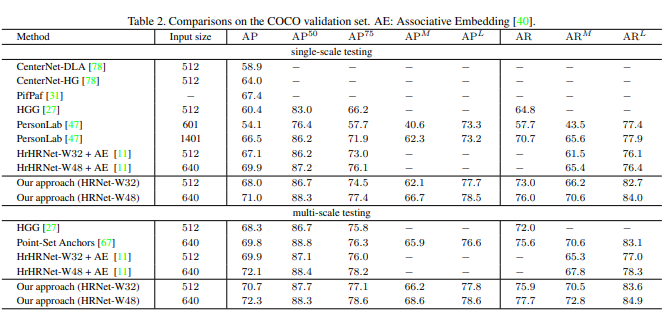
\includegraphics[scale = 0.6]{36}
\end{figure}
\begin{figure}[H]
	\centering
	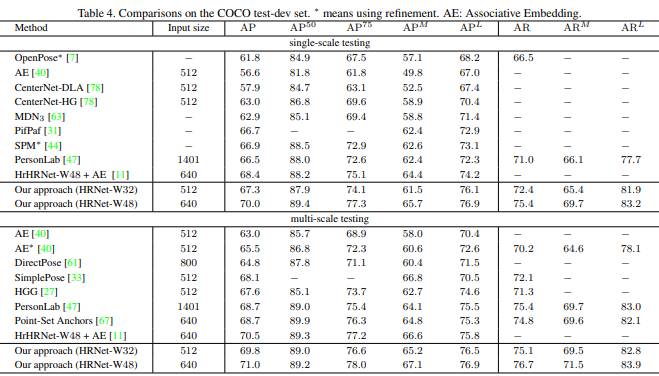
\includegraphics[scale = 0.6]{37}
\end{figure}
\begin{figure}[H]
	\centering
	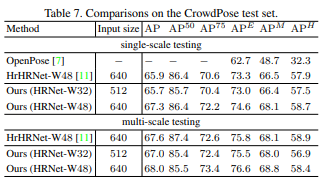
\includegraphics[scale = 0.6]{38}
\end{figure}
\section{Vision Transformer with Progressive Sampling}
$\text{https://github.com/yuexy/PS-ViT}$
\subsection{Abstract}
Transformers with powerful global relation modeling abilities have been introduced to fundamental computer vision tasks recently.

As a typical example, the Vision Transformer (ViT) directly applies a pure transformer architecture on image classification, by simply splitting images into tokens with a fixed length, and employing transformers to learn relations between these tokens.

However, such naive tokenization could destruct object structures, assign grids to uninterested regions such as background, and introduce interference signals. 

To mitigate the above issues, in this paper, we propose an iterative and progressive sampling
strategy to locate discriminative regions.

At each iteration, embeddings of the current sampling step are fed into a transformer encoder layer, and a group of sampling offsets is predicted to update the sampling locations for the next step.

Our proposed progressive sampling is differentiable.

\subsection{Introduction}
Reasearchers attempt to introduce them to fundamental computer vision tasks such as image classification,object detection and image segmentation.

However, transformers are initially tailored for processing mid-size sequences, and of quadratic
computational complexity w.r.t. the sequence length.

So they cannot directly be used to process images with massive pixels.

To overcome the computational complexity issue, the pioneer Vision Transformer(ViT) adopts a naive tokenization scheme that partitions one image into a sequence of regularly spaced patches, which are linearly projected into tokens. 

In this way, the image is converted into hundreds of visual tokens, which are fed into a stack of transformer encoder layers for classification. 

However, the limitations of such a naive tokenization scheme are obvious:

1.the hard splitting might separate some highly semantically correlated regions that should be modeled with the same group of parameters, which destructs inherent object structures and makes the input patches to be less informative.

2.tokens are placed on regular grids irrespective of the underlying image content.Most grids focus on the uninterested background, which might lead to the interesting foreground object is submerged in interference signals.

Instead of sampling from fixed locations,our proposed module updates the sampling locations in an iterative manner.

This mechanism utilizes the capabilities of the transformer to capture global information to estimate offsets towards regions of interest,by combining with the local contexts and the positions ofcurrent tokens.

PS-ViT pays more attentoin to foreground objects while less to ambiguous background compared with simple tokenization.
\begin{figure}[H]
	\centering
	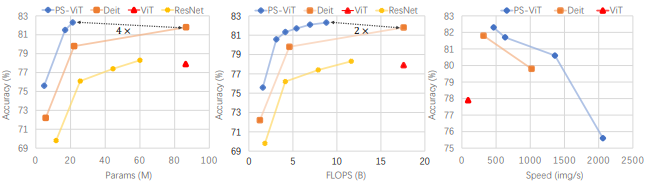
\includegraphics[scale = 0.6]{39}
\end{figure}
\subsection{Related Work}
Transformers are first proposed for squence models such as machine translation.It becomes atandard in many Natural Language Processing(NLP)tasks.

\subsubsection{Transformers in Computer Vision}
Many researchers attempt to apply transformers, or attention mechanism in computer vision tasks, such as image classification,object detection,image segmentation,low-level iamge processing,video understanding generation,multi-modality understanding,and Optical Character Recognition(OCR).

Axial attention applied attention along a single axis of the tensor without flattening to reduce the computational resource requirement.

iGPT simply down-sampled images to one low resolution, trained a sequence of transformers to auto-regressively predict pixels and achieved promising performance with a linear probe.

ViT regularly partitioned one high-resolution image into 16 × 16 patches,which were fed into one pure transformer architecture for classification.But ViT needs pretraining on large-scale datasets.

DeiT proposed a data efficient training strategy and a teacher-student distillation mechanism, and improved ViT’s performance greatly.

Our proposed PS-ViT also starts from ViT. Instead of splitting pixels into a small number of visual tokens, we propose a novel progressive sampling strategy to avoid structure destruction and focus more attention on interesting region

\subsubsection{Hard Visual Attention}
PS-ViT is differentiable and can be easily trained in an end-to-end fashion while previous hard visual attention approaches are non-differentiable and trained with Reinforcement Learning (RL) methods.

Our work is also related to the deformable convolution and deformable attention mechanism, however, the motivation and the way of pixel sampling in this work are different from what proposed in the deformable convolution and attention mechanism.

\subsection{Methodology}
\subsubsection{Progressive Sampling}
\begin{figure}[h]
	\centering
	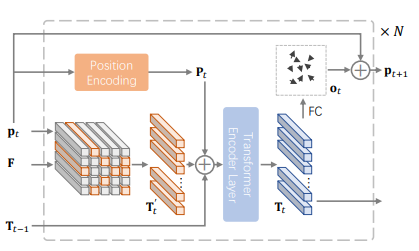
\includegraphics[scale = 0.7]{3}
\end{figure}
the feature map(F $\in \mathcal{R}^{C\times H\times W}$) extracted by the feature extractor module.Giving the sampling location $p_t\in \mathcal{R}^{2\times (n\times n)}$(the sampling points at the iteration t),where ($n\times n$) indicates the number of samples over one image and N is the total iterative number in the progressive sampling module.

For the first iteration, we  initialize the $p1$ to be the regularly-spaced locations.Concretely, the i-th location $p^i_1$(1 is the first iteration) is given by
$$\pi_i^y = \lfloor i/n\rfloor$$
$$\pi_i^x = i - \pi_i^y \times n$$
$$s_h = H/n$$
$$s_w = W/n$$
$$p_1^i = [\pi_i^ys_h + s_h/2,\pi_i^xs_w + s_w/2]$$
where $\pi_i^y$and $\pi_i^x$ map the location index i to the row index and the column one respectively.

Initial tokens are then sampled over the input feature map at the sampled locations as follows:
$$T'_t = F(p_t), t\in {1,...,N}$$
$T'_t\in \mathcal{R}^{C\times(n\times n)}$ are tokens sampled from F at the interation i.As elements of $p_t$ are fractional, the sampling is implemented via the bilinear interpolation operation.

$$P_t = W_tp_t$$
$$X_t = T'_x\oplus P_t \oplus T_{t-1}$$
$$T_t = Transformer(X_t), t\in {1,...,N}$$
$P_t\in \mathcal{R}^{C\times (n\times n)}$is the position embedding at the iteration t.$T'_t\in \mathcal{R}^{C\times (n\times n)}$is tokens sampled from F at the iteration t.$T_t\in \mathcal{R}^{C\times (n\times n)}$is tokens predicted by the progressive sampling module at the iteration t.$W_t\in \mathcal{R}^{C\times 2}$ is the linear transformation that projects the sampled location $p_t$ to the positional encoding matrix $P_t$ of size $C\times(n\times n)$,all iterations share the same $W_t$.Transformer(·) is the mulit-head self-attention based transformer encoder layer.
$$o_t = M_tT_t,t\in {1,...,N-1}$$
$M_t\in \mathcal{R}^{2\times C}$is the learnable linear transformation for predicting the sampling offset matrix.
\subsubsection{Overall Archtecture}

The architecture of the PS-ViT consists of four main components: 1) a feature extractor module to predict dense tokens; 2) a progressive sampling module to sample discriminative locations; 3) a vision
transformer module that follows the similar configuration of ViT and DeiT; 4) a classification module.

The feature extractor module aims at extracting the dense feature map F, where the progressive sampling module can simple tokens Tt. Each pixel of the dense feature map F can be treated as a token associated with a patch of the image.

\begin{figure}[h]
	\centering
	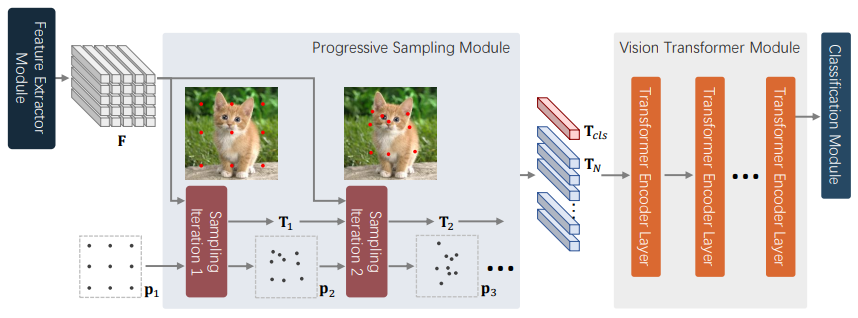
\includegraphics[scale = 0.7]{4}
\end{figure}
Given an input image, its feature map F is first extracted by the feature extractor module. Tokens $T_i$ are then sampled progressively and iteratively at adaptive locations $p_i$ over F in the progressive sampling module. The final output tokens $T_N$ of the progressive sampling module are padded with the classification token Tcls and further fed into the vision transformer module to refine $T_cls$, which is finally classified in the classification module.

We employ the convolutional stem and the first two residual blocks in the first stage of the ResNet50 as our feature extractor module.

We pad an extra token named by the classification token $T_{cls} \in \mathcal{R}^{C\times 1}$to the output tokens $T_N$ of the last iteration in the progressive sampling module, and feed them into the vision transformer module.And the output is $\mathcal{R}^{C\times (n\times n +1)}$

The vision transformer module follows the architecture adopted in ViT and DeiT.

The classification token refined through the vision transformer module is finally used to predict the image classes.
\subsubsection{Transformer Encoder Layer}
The transformer encoder layer serves as the basic building block for the progressive sampling module and the vision transformer module. Each transformer encoder layer has a multi-head self-attention and a feed-forward unit.

\section{PP-LCNet: A Lightweight CPU Convolutional Neural Network}

\subsection{Abstract}

This paper lists technologies which can improve network accuracy while the latency is almost constant. With these improvements, the accuracy of PP-LCNet can greatly surpass the previous network structure with the same inference time for classification

\subsection{Introduction}

As the model feature extraction capability increases and the number of model parameters and FLOPs get larger, it becomes difficult to achieve fast inference speed.

We consider the following three fundamental questions:
\noindent1.How to promote the network to learn stronger feature presentations without increasing latency.
\noindent2.What are the elements to improve the accuracy of lightweight models on CPU.
\noindent3.How to effectively combine different strategies for designing lightweight models on CPU.

We come up with several general rules for designing lightweight CNNs.

\subsection{Related Works}

Two types of methodologies to promote the capabilities of the models:
\noindent1.Manually-designed CNN Architecture.
\noindent2.Neural Architecture Search(NAS)

\subsubsection{Manually-designed Architecture}

VGG: Stacking blocks with the same dimension.

GoogLeNet: Inception block(including four parallel operation: 1 $\times$ 1 convolution, 3 $\times$ 3 convolution, 5 $\times$ 5 convolution and max pooling) which can make the convolution neural network light enough.

MobileNetV1: Depthwise and pointwise convolutions replace standard convolution.

MobileNetV2: Inverted block,which reduces the amount of parameters and FLOPs of the model.

ShuffleNetV1/V2: Exchange information through channel shuffle.

GhostNet: Ghost module, which can generate more feature maps with fewer parameters to improve the overall performance of the model.

\subsubsection{Neural Architecture Search}

MixNet: Hybridize depthwise converlations of different kernel size in one layer.

\subsection{Approach}

Here we have summarized some methods that can improve the performance of the model with little increase of inference time.

Concat or elementwise-add will not only slow down the inference speed of the model, but also will not improve the accuracy on a small model.

\begin{figure}[h]
	\centering
	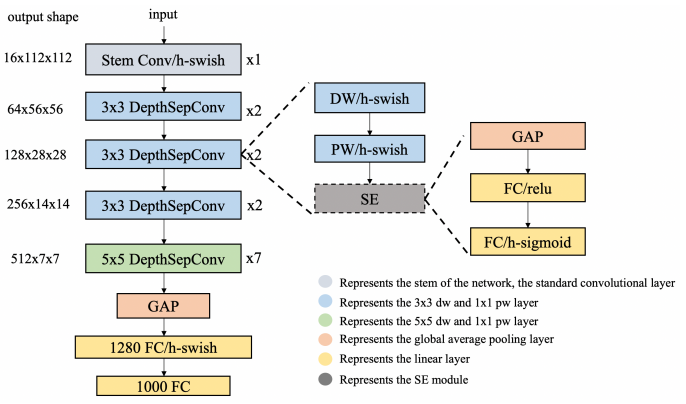
\includegraphics[scale = 0.5]{5}
\end{figure}
Stem Conv uses standard 3 $\times$ 3 convolution.DepthSepConv means depth-wise separable convolutions, DW means depth-wise convolution, PW means point-wise convolution, GAP means Global Average Pooling.
\subsubsection{Better Activation Function}

1.Sigmoid 2.ReLU 3.Swish activation funvtion 4.H-Swish

We replaced the activation function from ReLU to H-Swish.The performance has been grearly improved, while the inference time has hardly changed.

\subsubsection{SE Modules at Appropriate Position}

It does a good jib of weighting the network channels for better features,and its speed improvement version is also used in many lightweight networks.

The SE module increases the inference time,so that we cannot use it for the whole network.SE module is located at the end of the network,it can play a better role.So we just add the SE module to the blocks near the tail of the network.

The activation functions for the two layers of the SE module are ReLU and H-Sigmoid.

\subsubsection{Larger Convolution kernels}

The size of the convolution kernel often affects the final performance of the network.

However, mixing different sizes of convolutional kernels in the same layers of the network slows down the inference speed of the model, so we try to use only one size of convolution kernel in the single layer, and ensure that a large convolution kernel is used in the case of low latency and high accuracy.

We replace the 3 $\times$ 3 convolutional kernels with only the 5 $\times$ 5 convolutional kernels at the tail of the network would achieve the effect of replacing almost all layers of the network.
\subsubsection{Larger dimensional 1x1 conv layer after GPA}

When the output dimension of the network is small,in order to give the network a stronger fitting ability, we appended a 1280-dimensional size 1 $\times$ 1 conv(equivalent to FC layer) after the final GAP(Global Average Pooling) layer,which would allow for more storage of the model with little increase of inference time.

\subsection{Ablation Study}
\subsubsection{The impact of SE module in different positions}

\begin{figure}[h]
	\centering
	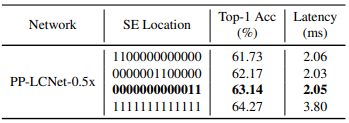
\includegraphics[scale = 0.5]{6}
\end{figure}
The table clearly shows that adding the last two blocks is more advantageous for almost the same inference time.
\subsubsection{The impact of large-kernel in different locations}

\begin{figure}[h]
	\centering
	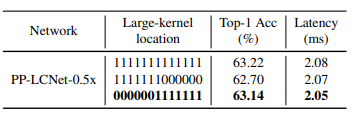
\includegraphics[scale = 0.5]{7}
\end{figure}
The table shows the positions added by the 5 $\times$ 5 depth-wise convolution.

1 means that the depth-wise convolution kernel in DepthSepConv is 5 $\times$ 5, and 0 means
that the depth-wise convolution kernel in DepthSepConv is 3 $\times$ 3.
\subsubsection{The impact of different techniques}

\begin{figure}[h]
	\centering
	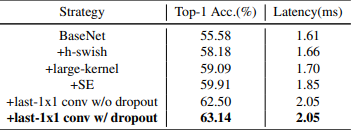
\includegraphics[scale = 0.5]{8}
\end{figure}
At the same time, perhaps because a relatively large matrix is involved here, the use of the dropout strategy can further improve the accuracy of the model.
\subsection{Conclution and Future Work}

The CNN used the approach shows stronger performance on a large number of vision tasks and has a better accuracy-speed balance.

In addition, this work reduces the search space of NAS and also offers the possibility of faster access to lightweight models for NAS.

In the future, we will also use NAS to obtain faster and stronger models.
\section{FCPose: Fully Convolutional Multi-Person Pose Estimation with Dynamic Instance-Aware Convolutions}
\subsection{Abstract}
We propose a fully convolutional multi-person pose estimation framework(FCPose) using dynamic instance-aware convolutions.

Moreover, with the strong representation capacity of dynamic convolutions, the keypoint heads in FCPose are designed to be very compact, resulting in fast inference and making FCPose have almost constant inference time regardless of the number of persons in the image.

FCPose also offers better speed/accuracy trade-off than other state-of-the-art methods.(most important thing is the speed and infer time)

\subsection{Introduction}
Detecting each individual instance with a person detector often get the detected boxes from the ROIs.

An ROI operation is used to crop the person from either the feature maps or the original image.Then single person keypoint detection is performed within a ROI for each person, individually.

Some drawbacks about ROI-based pipeline:
\noindent1.the ROIs are forwarded separatedly and thus converlutional computation cannot be shared.(the inference time depends on the number of instances in the image)
\noindent2.top-down methods usually are not end-to-end trainable since the ROIs are often obtained from an isolated person detector.Moreover the inference time is longer.
\noindent3.these ROI-based methods also rely on the localization quality of the ROIs.

Some drawbacks about bottom-up methods:the processing of assembling the keypoints is usually heuristic and can involves many hyperparameters that make methods complicated.

The key idea of our solution is to use the keypoint heads whose convolution filters/weights are dynamically generated.

More specifically, for each instance, we dynamically generate a keypoint head. The generated keypoint head is applied to convolutional feature maps in the fashion of fully convolutional networks.

This is made possible as the keypoint head can encode the instance's characteristics in the filters' weights.Thus, this keypoint head can distinguish the instance's keypoints from that of other instances, hence instance-specific convolution filters.

The localization precision of keypoint detection is tightly related to the output resolution of the FCN(Full Convolutional Network).

Typically, the output resolution of the fully convolutional keypoint heads is designed to that of
the input feature maps(e.g. $\frac{1}{8}$),but it is not sufficient for ketpoint detection.If simply using deconvolutions would inevitably result in significantly increased computation overhead.

If we upsample the heatmaps by 8 times, the memory footprint will be increased by 64 times. Also, this will result in much longer computational time.
\subsection{Contributions}
1.We propose an efficient and accurate FCPose bulit upon dynamic filters.For the first time, we demonstrate that an ROI-free and grouping-free end-to-end trainable human pose estimator can achieve even better accuracy and speed, comparing favourably with recent top-down and bottom-up methods.

2.Not using ROIs also avoids that the keypoint prediction is truncated by the inaccurate detected boxes.

3.The core of FCPose is the use of the dynamic filters in our keypoint heads. Dynamically generated filters have demonstrated strong representation capacities.Thus ,we only need a small number of such convolutions for achieving top results and the overall inference time is fast.

\subsection{Related Work}
Compared to top-down methods, bottom-up methods are often faster because it computes all the convolutional features once, being fully convolutional models.

\textbf{Top-down}:

A single-person estimation method is applied to the cropped image patch to attain keypoint locations. These methods can work well. 

The main drawback is the slow inference speed because they do not share the computation and features with the person detector.

The second-stage pose estimation can be very slow when the number of person instances in the image is large.

Mask R-CNN proposes the ROIAlign operation, which can directly obtain the features of the ROIs from the feature maps of the detector. Thus, it can share the features between the ROIs and the detector,significantly speeding up the inference.

\textbf{Botton-up}:
Detecting all the keypoints in an instance-agnostic fashion, and then a grouping post-processing is used to obtain the instance-level keypoints.

\textbf{Dynamic filters and conditional convolutions}
This is different from the traditional convolutional networks, whose weights are fixed once trained.

Moreover, the dynamic filters can be conditioned on each instance in the image, which can make
the filters only fire for the target instance. Thus, it can be viewed as a new operation that makes a model attend to the instance, thus replacing the previous ROI operations.

\subsection{Approach}
\subsubsection{Overall Architecture}
Challenge in multi-person keypoints:the vanilla FCNs cannot produce instance-aware keypoints.

Formally let G $\in \mathcal{R}^{h\times w\times K}$be the features of an ROI, and $f_\theta$be the keypoint head,$\theta$is the learnable network weights.(The ROI operation is the core operation making the model attend to an instance)

Note that K being 17 on COCO is the number of keypoints for an instance.

Then, the final keypoint coordinates can be obtained by finding the peak on each channel of the
heatmaps.

For each instance, i, a new set of weights $\theta_i$ of the keypoint head will be generated. The
keypoint head with weights $\theta_i$ is applied to full-image feature maps.

In this work, we use FCOS to generate the dynamic weights $\theta_i$ for each instance. To this end, we add a new output branch to the box regression branch of FCOS.

Formally let F$\in \mathcal{R}^{H\times W\times 32}$be a level of feature maps and have the same resolution of $P_3$ in the FPN(Feature Parymid Network).

For the instance i,the predicted heatmaps $H\in \mathcal{R}^{H\times W\times K}$are $H = f_{\theta_i}(F)$.

F is the full-image feature maps without any cropping operations.The filters' weights $\theta_i$ are conditioned on the features of the instance i and thus it can encode the characteristics of the target instance.
\begin{figure}[h]
	\centering
	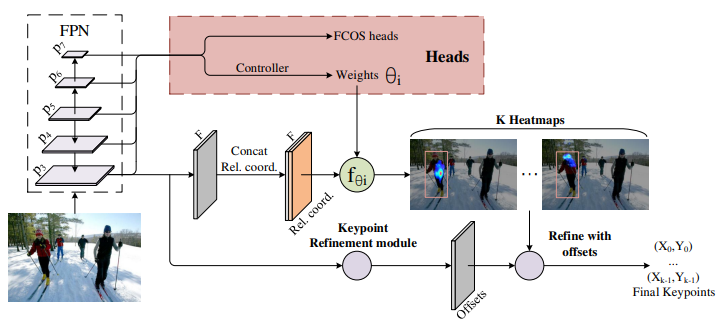
\includegraphics[scale = 0.5]{9}
\end{figure}

FCPose is built on the one-stage object detector FCOS. The controller that generates the weights of the keypoint heads is attached to the FCOS heads. 

The weights $\theta_i$ generated by the controller is used to fulfill the keypoint head f for the instance i. Moreover, a keypoint refinement module is introduced to predict the offsets from each location of the heatmaps to the ground-truth keypoints. 

Finally, the coordinates derived from the predicted heatmaps are refined by the offsets
predicted by the keypoint refinement module, resulting in the final keypoint results.

“Rel. coord.” is a map of the relative coordinates from all the locations of the feature maps F to the location where the weights are generated. The relative coordinate map is concatenated to F as the input to the keypoint head.

\begin{figure}[h]
	\centering
	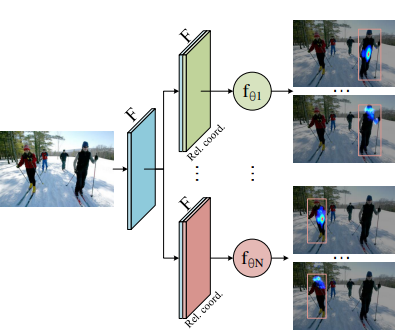
\includegraphics[scale = 0.5]{10}
\end{figure}

The core idea of the dynamic keypoint head in FCPose. F denotes a level of feature maps. “Rel. Coord.”means the relative coordinates, denoting the relative offsets from the locations of F to the location where the filters are generated.

\subsubsection{Keypoint Refinement with Regression}
If we upsample the heatmaps by 8 times, the memory footprint will be increased by 64 times. Also, this will result in much longer computational time.

Here, we address this issue by introducing a regression-based keypoint refinement module. 

Let $O\in \mathcal{R}^{H\times W\times 2K}$be the output feature maps of the module. $O_{i,j} = (\Delta x,\Delta y)$ predicts the offsets from the location(i.j) to the nearest groundtruth keypoint.As a result, for a keypoint, if its heatmap’s peak is at (i, j), the final coordinates of the keypoint will be $(i + \Delta x,j + \Delta y)$.

\subsubsection{Training Targets and Loss Functions}
\textbf{Training targets:}

First, we use the same processing to associate each location on the feature maps with an instance or label the location negative.

The classification and box regression training targets of each location are computed as in FCOS.

A location is also required to generate the keypoint head’s filters(not explicitly supervised) for the associated instance.

In FCOS, for each batch of images (on the same GPU), we might have up to 500 positive locations.(If all these locations are used to generate the filters, it will come with high computational overheads.)

Therefore, for each batch, we only sample at most M = 50 positive locations with high confidence to generate filters.

\textbf{Loss Functions:}

The loss functions of FCPose consisit of three parts:$L_{fcos}$,$L_{heatmap}$,$L_{reg}$

$$L_{fcos} = L({p_{x,y}},{t_{x,y}}) = \frac{1}{N_{pos}}\sum_{x,y}L_{cls}(P_{x,y},c_{x,y}^*) + \frac{\lambda}{N_{pos}}\sum_{x,y}I_{c_{x,y}^*>0}L_{reg}(t_{x,y},t_{x,y}^*)$$
$L_{cls}$ is focal loss. $L_{reg}$ is the IOU loss.$N_{pos}$ denotes the number of positive samples and $\lambda$ being 1 to balance weight for $L_{reg}$.The summation is calculated over all locations on the feature maps $F_i$.$I_{c_{x,y}^*>0}$ is the indicator function,being 1 if $c
^∗_i \textgreater 0$ and 0 otherwise.


$$L_{heatmap} = CE(softmax(H_i),H^*)$$
CE(cross entropy). To be specific, assume a ground-truth keypoint’s coordinates are ($x^*,y^∗$), and the heatmap’s resolution is $\frac{1}{8}$ resolution of the input image.Then, for this keypoint, the location $\left \lfloor \frac{x-4}{8}\right \rfloor, \left \lfloor \frac{y-4}{8}\right \rfloor$on its ground-truth heatmap will be set 1 and other locations will be zeros.

we refine the coordinates of the peak by the offsets of the keypoint regression module, and obtain
the resulting keypoint coordinates. Finally, non-maximum suppression (NMS) is used to remove the duplicates.

$H_i^* \in \mathcal{R}^{H\times W}$ be the ground-truth heatmap for the keypoint.$H_i \in \mathcal{R}^{H\times W}$ is the heatmap predicted by the dynamic keypoint head for this keypoint.

$$L_{reg} = \frac{1}{n}\sum_{i=1}^{m}w_i(y_i - \hat{y_i})^2$$
MSE(mean square error) is used to compute the difference between the predicted offsets and groundtruth ones for the keypoint offset regression.

Overall loss function:
$$L_{overall} = L_{fcos} + \alpha L_{heatmap} + \beta L_{reg}$$
$\alpha,\beta$are the loss weights, respectively.
\subsection{Ablation Experiments}
\subsubsection{Architecture of the Dynamic Keypoint Head}
The effect of the number of channels of the input feature maps to the keypoint head
\begin{figure}[H]
	\centering
	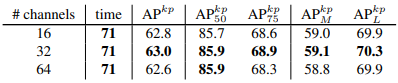
\includegraphics[scale = 0.5]{11}
\end{figure}
Varying the number of the layers in the dynamic keypoint head.
\begin{figure}[H]
	\centering
	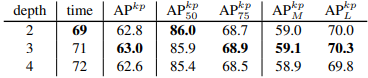
\includegraphics[scale = 0.5]{12}
\end{figure}
The effect of the number of channels in the dynamic keypoint head
\begin{figure}[H]
	\centering
	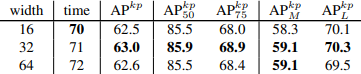
\includegraphics[scale = 0.5]{13}
\end{figure}
Comparison of various upsampling methods on the COCO val2017 split.
\begin{figure}[H]
	\centering
	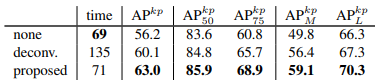
\includegraphics[scale = 0.5]{14}
\end{figure}
Share the keypoint refinement module between instances or not.
\begin{figure}[H]
	\centering
	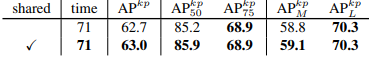
\includegraphics[scale = 0.5]{15}
\end{figure}
Comparisons with recent state-of-the-art methods.
\begin{figure}[H]
	\centering
	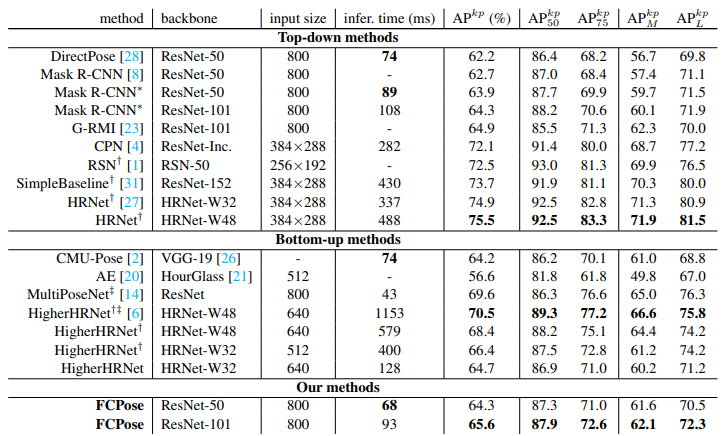
\includegraphics[scale = 0.5]{16}
\end{figure}
\subsection{Conclusions}
FCPose can eliminate the ROI operations in top-down methods and the grouping post-processing in
bottom-up methods, solving keypoint detection in the fully convolutional fashion.

\begin{figure}[H]
	\centering
	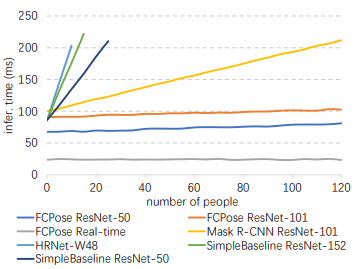
\includegraphics[scale = 0.5]{17}
\end{figure}

The core idea of FCPose is to use the dynamic keypoint head instead of ROIs to make the model attend to instances.
\section{Polarized Self-Attention: Towards High-quality Pixel-wise Regression}
\subsection{Abstract}
Pixel-wise regression is probably the most common problem in fine-grained computer vision tasks, such as estimating keypoint heatmaps and segmentation masks.

Attention mechanisms in Deep Convolutional Neural Networks(DCNNs) has become popular for boosting
long-range dependencies, element-specific attention.

We present the Polarized Self-Attention(PSA) block that incorporates two critical designs towards highquality pixel-wise regression:

\noindent1.Polarized filtering: keeping high internal resolution in both channel and spatial attention computation while completely collapsing input tensors along their counterpart dimensions

\noindent2. Enhancement:composing non-linearity that directly fits the output distribution of typical fine-grained regression, such as the 2D Gaussian distribution (keypoint heatmaps), or the 2D Binormial distribution (binary segmentation masks).

\subsection{Introduction}
Comparing to the coarse-grained tasks, perception at the pixel-wise level is increasingly appealing

The goal of the pixel-wise regression problem is to map every image pixels of the same semantics to the same scores.

The encoder usually consists of a backbone network,such as ResNet [18], that sequentially reduces the spatial resolution and increases the channel resolution, while the decoder usually contains de-convolution/up-sampling operations that recover the spatial resolution and decrease the channel resolution

The pixel appearances and patch shapes of the same semantics are highly nonlinear in nature and therefore difficult to be encoded with a reduced number of features

From the model design perspective, the pixel-wise regression problem faces special challenges:

\noindent1.Keeping high internal resolution at a reasonable cost

\noindent2.Fitting output distribution.

Channel-only attention(SE,GE,DA,CBAM,GCNet) in classification task(put the same weights on different spatial location and its spatial information eventually collapses by pooling) and in object detection task(the channel-only attention unanimously highlights all foreground pixels)

PSA fuse softmax sigmoid composition in both channel-only and spatial-only attention branches.
\subsection{Related Work}
\subsubsection{Pixel-wise Regression Tasks}
Other most recent variants, DARK-Pose and UDP-Pose, both compensate for the loss of resolution due to the preprocessing, post-processing, and propose techniques to achieve a sub-pixel estimation of keypoints.

PSA further pursues the high-resolution goals of the above efforts from the attention perspective and further boosts the above DCNNs.
\subsubsection{Self-attention and its Variants}
Attention mechanisms have been introduced into many visual tasks to address the weakness of standard convolutions.

In the self-attention mechanism, each input tensor is used to compute an attention tensor and is then re-weighted by this attention tensor.

PSA advances self-attention for pixel-wise regression and could also be used in other variants such as the convolution-augmented attentions.
\subsubsection{Full-tensor and simplified attention blocks}
The basic non-local block (NL) and its variants, such as a residual form second-order non local, and asymmetric non-local, produce full-tensor attentions and have successfully improved person re-identification, image super-resolution, and semantic segmentation tasks.

NL block lead to huge memory and computational costs.

BAM,DAN and CBAM produce different compositions of the channel-only and spatial-only attentions. Squeeze-and-Excitation (SENet), GatherExcite and GCNet only re-weight feature channels using signals aggregated from global context modeling.

PSA address the specific challenges in fine-grained regression by keeping the highest attention resolution among existing attention blocks, and directly fitting the typical output distributions.

\subsection{Method}
\subsubsection{Self-Attention for Pixel-wise Regression}
A DCNN for pixel-wise regression learns a weighted combination of features along two dimensions: 

\noindent(1) channel specific weighting to estimate the class-specific output scores;

\noindent(2) spatial-specific weighting to detect pixels of the same semantics.

In the Non-Local self-attention with a full-tensor self-attention the highlighting could potentially
be achieved at the element-wise granularity ($C\times H\times W$ elements)
$$Z = A(X)\odot X \quad (A(X) \in \mathcal{R}^{C\times H\times W})$$
However, the attention tensor A is very complex and noise-prone to learn directly.

And the A is calculated as,
$$A = W_z(F_{sm}(X^TW_k^TW_qX)W_vX)$$
$W_z,W_k,W_q,W_v$that learns the linear combination of spatial features among different channels are four $1\times1$ convolution kernels.

Within the same channels,$W_kX$ and $W_qX$ activates any features at different spatial locations that have a similar intensity.

The joint activation mechanism of spatial features is very likely to highlight the spatial noise.

The only actual weights, $W_s$, are channel-specific instead of spatial-specific, making the Non-Local attention exceptionally redundant at the huge memory-consumption of the $HW \times HW$ matrix.

Low rank approximation(SVD function:Take the k principal components in front of A) of A (EA), Channel-only self-attention $A^{ch}\in \mathcal{R}^{C\times1\times1}$ that highlight the same global context for all pixels(GC and SE)

Spatial-only self-attention $A^{sp}\in \mathcal{R}^{1\times W\times H}$  is not powerful enough to be recognized as a standalone model.

\noindent Parallel composition: $Z = A^{ch} \odot^{ch} X + A^{sp} \odot^{sp}X$

\noindent Sequential composition: $Z = A^{ch} \odot^{ch}(A^{sp} \odot^{sp} X)$

Different conclusions were empirically drawn, such as CBAM(sequential>parallel) and DA (parallel>sequential),which partially indicates that the intended non-linearity of the tasks are not fully modeled within the attention blocks.(pixel-wise regression)

Using these backbones in pixel-wise regression, self-attention blocks are expected to preserve high-resolution semantics in attention computation.

\begin{figure}[h]
	\centering
	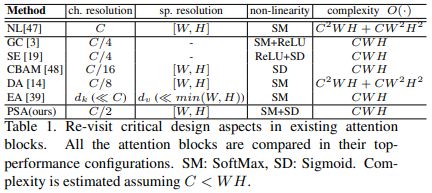
\includegraphics[scale = 0.5]{18}
\end{figure}

are there better non-linear that could leverages higher resolution information in attention computation?

In my opinion, polarized self-attention mechanism can maintain good performance in fine-grained pixel-level tasks, which largely depends on its lack of compression in space and channel dimensions, resulting in relatively small information loss.

In addition, previous attention methods used only Softmax or Sigmoid for probability estimation using nonlinear functions. In order to fit the output distribution of fine-grained regression results, the polarization self-attention mechanism adopts Softmax and Sigmoid functions in both channel and spatial branches.

\subsubsection{Polarized Self-Attention(PSA)Block}
The propose the Polarized Self-Attention(PSA)mechanism:

\noindent 1.Filtering: completely collapse features in one direction while preserving high-resolution in its orthogonal direction.

\noindent 2.HDR(High Dynamic Range): increase the dynamic range of attention by Softmax normalization at the bottleneck tensor (smallest feature tensor in attention block), followed by tone-mapping with the Sigmoid function.)
\begin{figure}[h]
	\centering
	\begin{minipage}{0.45\textwidth}
		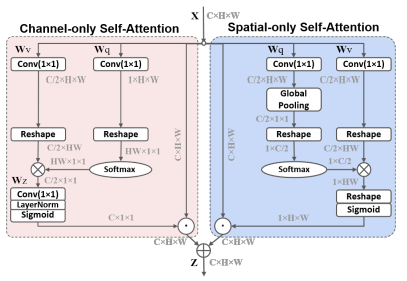
\includegraphics[scale = 0.5]{19}
		\caption{the parallel layout}
	\end{minipage}
\quad
	\begin{minipage}{0.45\textwidth}
		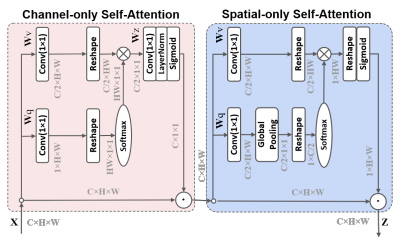
\includegraphics[scale = 0.5]{20}
		\caption{the sequential layout}
	\end{minipage}
\end{figure}

\textbf{Channel-only branch}: $A^{ch}(X) \in \mathcal{R}^{C\times 1\times 1}$

$$A^{ch}(X)=F_{SG}[W_{z|\theta_1}(\sigma_1(W_v(X))\times F_{SM}(\sigma_2(W_q(X))))]$$

$W_z,W_q,W_v$ are four(1 x 1)convolution kernels and they learn the linear combination of spatial
features among different channels.$\sigma_1$ and $\sigma_2$ are two tensor reshape operators.$F_{SM}$ is a SoftMax operator and $\times$ is the matrix dot-product operation.

The output of channel-only branch is $Z^{ch}=A^{ch}(X)\odot^{ch}X\in \mathcal{R}^{C\times H\times W}$,$\odot^{ch}$ is a channel-wise multiplication operator.

\textbf{Spatial-only branch}: $A^{sp}(X) \in \mathcal{R}^{1\times H\times W}$

$$A^{sp}(X)=F_{SG}[\sigma_3(F_{SM}(\sigma_1(F_{GP}(W_q(X))))\times \sigma_2(W_q(X)))]$$

$W_q$ and $W_v$ are standard $1\times 1$ convolution layers respectively.$\sigma_1$ $\sigma_2$ and $\sigma_3$ are three tensor reshape operators. $F_{SM}$ is the SoftMax operator, $F_{GP}$ is a globel pooling operator.$\times$ is the matrix dot-product operation.

The output of spatial-only branch is $Z^{sp}=A^{sp}(X)\odot^{sp}X\in \mathcal{R}^{C\times H\times W}$,$\odot^{sp}$ is a spatial-wise multiplication operator.

\textbf{Composition:}PSA also have two layouts.

\noindent parallel layout: 
$$PSA_p(X) = Z^{ch}+Z^{sp} = A^{ch}(X\odot^{ch}X + A^{sp}(X)\dots^{sp}X$$
(+ is the element-wise addition operator)
\noindent sequential layout:
$$PSA_s(X) = Z^{sp}(Z^{ch}) = A^{sp}(A^{ch}(X)\odot^{ch}X)\odot^{sp}A^{ch}(X)\odot^{ch}X$$

We add PSAs after the first 3 × 3 convolution in every residual block.
\subsection{Ablation Study}
\begin{figure}[h]
	\centering
	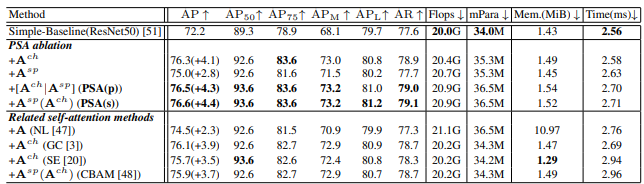
\includegraphics[scale = 0.5]{21}
\end{figure}
From the results, we can observe:

1.the NL block costs the most memory while produces the least boost (2.3AP) over the baseline, indicating that NL is highly redundant. 

2.The channel-only attention GC is better than SE since it includes SE. GC is even better than channel+spatial attention CBAM because the inner-product-based attention mechanism in GC is more
powerful than the convolution/MLP-based CBAM.

3.PSA $A^{ch}$ is the best channel-only attention block over GC and SE. We believe PSA benefits from its highest channel resolution (C/2) and its output design.

4.The channel+spatial attention CBAM with a relatively early design is still better than the channel-only attention SE.

5.Under the same sequential layout of spatial and channel attention, PSA is significantly better than CBAM.

6.At similar overheads, both the parallel and sequential PSAs are better than the compared blocks.

\begin{figure}[H]
	\centering
	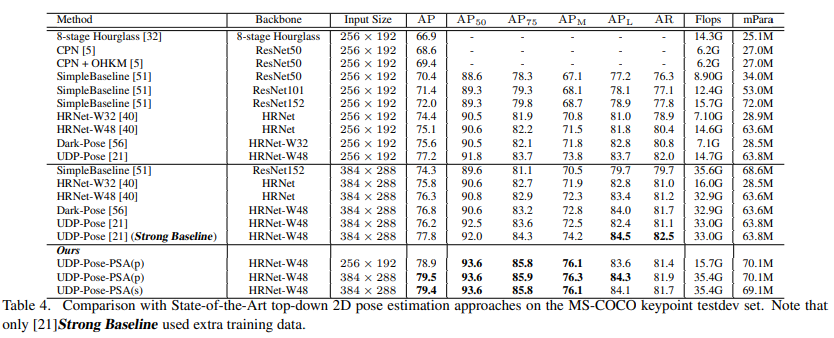
\includegraphics[scale = 0.5]{22}
\end{figure}
\subsection{Conclusion and Future Work}
PSA significantly boosts all compared DCNNs for two critical designs:

(1)keeping high internal resolution in both polarized channel-only and spatial-only attention branches.

(2)incorporating a nonlinear composition that fully leverages the high-resolution information preserved in the PSA branches.

Our future work is to explore the use of PSAs in DCNN heads.
\section{The Devil in the Details: Delving into Unbiased Data Processing for Human Pose Estimation}
$\text{https://github.com/HuangJunJie2017/UDP-Pose}$
\subsection{Abstract}
Recently, the leading performance of human pose estimation is dominatedby top-down methods.

We find that the results obtained by common flipping strategy are unaligned with the original ones in inference.

Moreover, there is statistical error in standard encoding-decoding during both training and inference.

Data is processed in continuous space based on unit length (the intervals between pixels) instead of in discrete space with pixel, and a combined classification and regression approach is adopted to
perform encoding-decoding.

The Unbiased Data Processing (UDP) for human pose estimation can be achieved by combining the two together.
\begin{figure}[H]
	\centering
	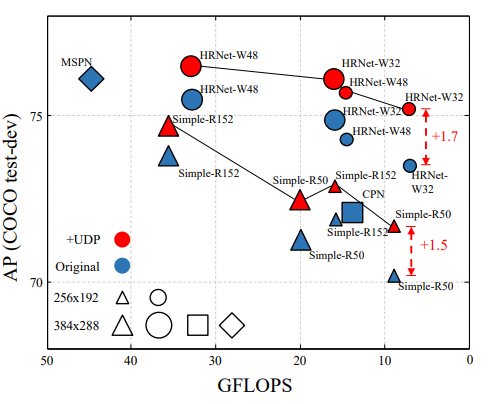
\includegraphics[scale=0.5]{23}
\end{figure}
\subsection{Introduction}
In the evaluation of human pose estimation, the metrics are calculated based on the positional offset between ground truth labels and prediction results, where small systematic bias caused by data processing will degrade the performance of pose estimators.

We find that most state-of-the-art systems suffer from the same two common problems:
\noindent 1.The unaligned results in inference obtained by using flipping strategy, which is derived from analyzing this problems in discrete space and utilizing pixel to measure the size of images in data transformation.
\noindent 2.Statistical error in standard encoding-decoding during the training and inference, repectively.

Based on the analysis results, a principled Unbiased Data Processing (UDP) is proposed to tackle this dilemma.

It is worth noting that UDP is a model-agnostic approach, which can serve for most top-down pipelines.

\subsection{Contributions}
1.This paper quantitatively analyzes the common biased data processing for human pose estimation. Interestingly, we find that the systematic error in standard data transformation and encoding-decoding couple together and significantly degrade the performance of top-down
pipelines. To the best of our knowledge, this is the first work to systematically address the data processing in pose community.

2.Based on analysis results, this paper formulates a principled Unbiased Data Processing (UDP) strategy, which equips with unit length-based measurement and combined classification and regression encoding-decoding. The proposed UDP is a model-agnostic strategy and can be utilized in most top-down pose estimators. We hope UDP will be significant for result
reproducing and future research.

3.On challenging COCO human pose estimation dataset,UDP promotes state-of-the-arts by large margin among variable backbones and input sizes.
\subsection{Related Work}
As single person pose estimation is performed with fixed scale patches, most state-of-the-art performances on multi-person popular benchmarks are achieved by top-down methods.

\textbf{Bottom-up Methods:}

\noindent 1.OpenPose builds a model that contains two branches to predict keypoint heatmaps and pairwise relationships (part affinity fields) between them.

\noindent 2.(Associative embedding: End-to-end learning for joint detection and
grouping)use one network for both heatmap prediction and grouping. Grouping is done by association embedding, which assigns each keypoint with a tag and groups keypoints based on the L2 distance between tag vectors.

\noindent 3.MultiPoseNet simultaneously achieves human detection and pose estimation, and proposes PRN to group the keypoints by the bounding box of each people.

\noindent 4.HighterHRNet maintains high-resolution feature maps which effectively improves the precision of the predictions.

\textbf{Top-down Methods:}

\noindent 1.CPN and MSPN are the leading methods on COCO keypoint challenge, adopting cascade network to refine the keypoint challenge, adopting cascade network to refine the keypoints prediction.

\noindent 2.SimpleBaseline adds a few deconvolutional layers to enlarge the resolution of output features.It is simple but effective in performance improvement.

\noindent 3.HRNet maintains high-resolution representations through the whole process,achieving state-of-the-art performance on public dataset.

\noindent 4.Mask R-CNN builds an end-to-end framework and achieving a good balabe between performance and inference speed.

\textbf{Data Processing in Human Pose Estimation:}
Top-down paradigm mainly includes data transformation, data augmentation and encoding-decoding.

\noindent 1.Data transformation:Transforming the keypoint location between different coordinate systems such as source image, network input and output.(Using pixel to measure the size of images,leading to unaligned results when using flipping strategy in inference.)

\noindent 2.Data augmentation:A common strategy for increasing the diversity of samples, which can do help to enhance the robustness of the algorithms.

\noindent 3.Encoding-decoding:In training process, they encode the ground truth into a heatmap with Gaussian distribution centered at the keypoint position.Decode means transforming the network predicted heatmap back into keypoint coordinate in inference process.

\subsection{Unbiased Data Processing for Human Pose Estimation}
We analyze the standard data processing approaches in current state-of-the-arts from two aspects:data transformation and encoding-decoding.
\subsubsection{Data Transformation}
The data transformation means transforming the keypoint location such as cropping, rotation, resizing and flipping between different coordinate systems.

\noindent \textbf{Standard Data Transformation:}
Using the pixel as the measurement would significantly degrade the performance when the
de facto standard flipping strategy is performed during inference.

\begin{figure}[H]
	\centering
	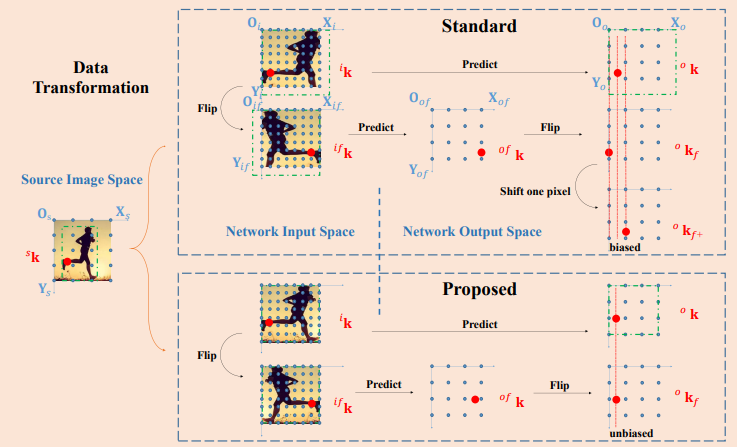
\includegraphics[scale=0.5]{40}
\end{figure}
\subsection{Future Work}
Future work will apply the proposed UDP to face landmark, anchor-free object detection and 3D human pose estimation
\section{A ConvNet for the 2020s}
$\text{https://github.com/facebookresearch/ConvNeXt}$
\subsection{Abstract}
It is the hierarchical
Transformers (e.g., Swin Transformers) that reintroduced several ConvNet priors, making Transformers practically viable as a generic vision backbone and demonstrating remarkable performance on a wide variety of vision tasks.

However,the effectiveness of such hybrid approaches is still largely credited to the intrinsic superiority of Transformers, rather than the inherent inductive biases of convolutions

In this work, we reexamine the design spaces and test the limits of what a pure ConvNet can achieve. We gradually “modernize” a standard ResNet toward the design of a vision Transformer,and discover several key components that contribute to the performance difference along the way.
\subsection{Introdution}
\begin{figure}[H]
	\centering
	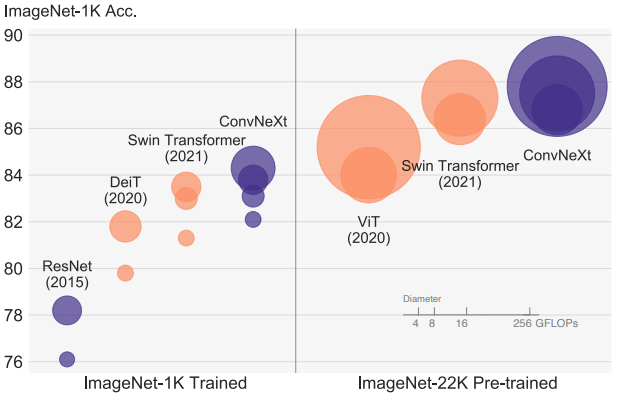
\includegraphics[scale=0.5]{41}
\end{figure}

The full dominance of ConvNets in computer vision was not a coincidence: in many application scenarios, a “sliding window” strategy is intrinsic to visual processing, particularly when working with high-resolution images. ConvNets have several built-in inductive biases that make them wellsuited to a wide variety of computer vision applications, the computions are shared.

One primary focus of ViT is on the scaling behavior: with the help of larger model and dataset sizes, Transformers can outperform standard ResNets by a significant margin.

The biggest challenge is ViT’s global attention design, which has a quadratic complexity with respect to the input size.This might be acceptable for ImageNet classification, but quickly becomes intractable with higher-resolution inputs.

Swim Transformer is a milestone work in the "sliding window" strategy(e.g. sttenttion within local windows) was reintroducted.

Under this perspective, many of the advancements of Transformers for computer vision have been aimed at bringing back convolutions.These attempts, however, come at a cost: a naive implementation of sliding window self-attention can be expensive; with advanced approaches such as cyclic shifting, the speed can be optimized but the system becomes more sophisticated in design.

ConvNets and hierarchical vision Transformers become different and similar at the same time: they are both equipped with similar inductive biases, but differ significantly in the training procedure and macro/micro-level architecture design.

Our research is intended to bridge the gap between the pre-ViT and post-ViT eras for ConvNets, as well as to test the limits of what a pure ConvNet can achieve.
\subsection{Modernizing a ConvNet: a Roadmap}
\begin{figure}[H]
	\centering
	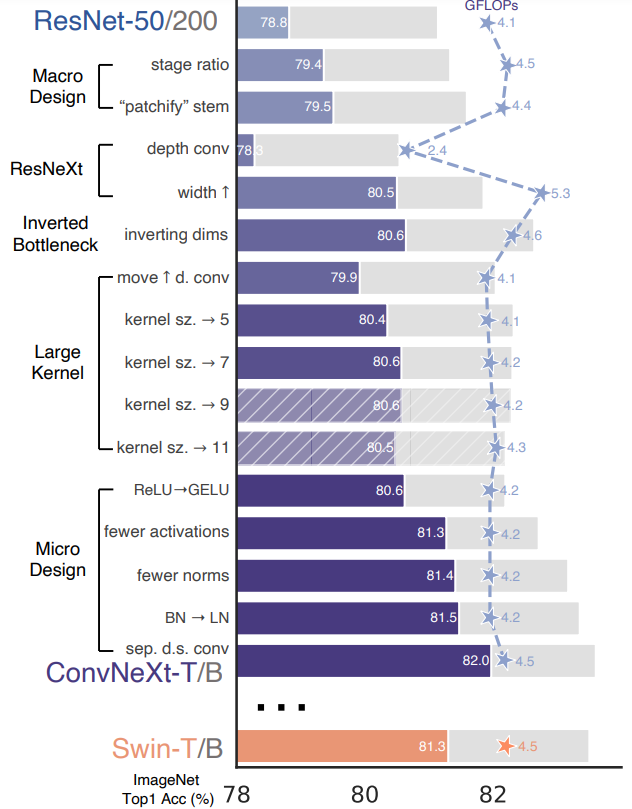
\includegraphics[scale=0.5]{42}
\end{figure}
We then study a series of design decisions which we summarized as 1) macro design, 2) ResNeXt, 3) inverted bottleneck, 4) large kernel size, and 5) various layer-wise micro designs.

In the figure,we show the procedure and the results we are able to achieve with each step of the “network modernization”.
\subsubsection{Tranining Techniques}
This pertains mostly to the optimization strategy and associated hyper-parameter settings.Thus, the first step of our exploration is to train a baseline model with the vision Transformer training procedure.

\begin{figure}[H]
	\centering
	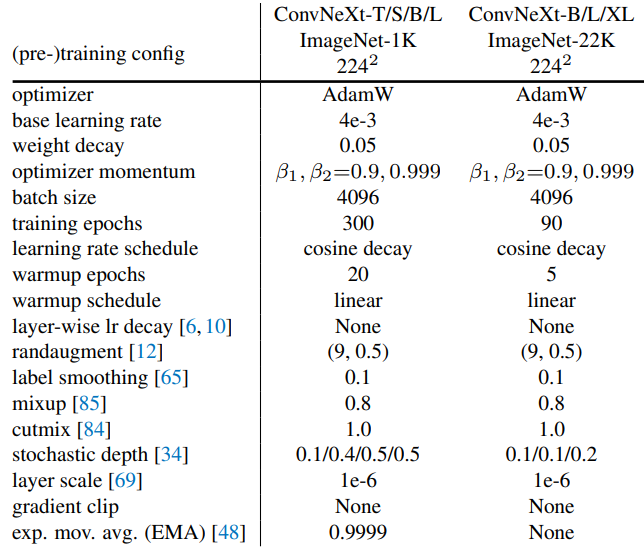
\includegraphics[scale=0.5]{43}
\end{figure}
\subsubsection{Macro Design}
There are two interesting design considerations: the stage compute ratio, and the “stem cell” structure.

\textbf{Changing stage compute ratio:}

Following the design, we adjust the number of blocks in each stage from (3, 4, 6, 3) in ResNet-50 to (3, 3, 9, s3), which also aligns the FLOPs with Swin-T.

\textbf{Changing stem to Patchify:}

We replace the ResNet-style stem cell with a patchify layer implemented using a 4×4, stride 4 convolutional layer.
\subsubsection{ResNeXt-ify}
The core component is grouped convolution, where the convolutional filters are separated into different groups.

We note that depthwise convolution is similar to the weighted sum operation in self-attention, which operates on a per-channel basis.

Following the strategy proposed in ResNeXt, we increase the network width to the same number of channels as Swin-T’s (from 64 to 96).

\subsubsection{Inverted Bottleneck}
Despite the increased FLOPs for the depthwise convolution layer, this change reduces the whole network FLOPs to 4.6G, due to the significant FLOPs reduction in the downsampling residual blocks’ shortcut 1×1 conv layer.
\begin{figure}[H]
	\centering
	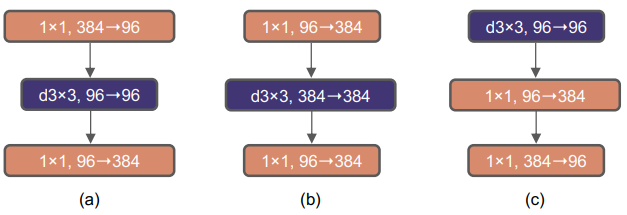
\includegraphics[scale=0.5]{44}
\end{figure}
(a) is a ResNeXt block.(b) we create an inverted bottleneck block.(c) the position of the spatial depthwise conv layer is moved up.

\subsubsection{Increasing the kernel size}
With all of these preparations, the benefit of adopting larger kernel-sized convolutions is significant.We will use $7\times 7$ depthwise conv in each block.

\subsubsection{Replacing ReLU with GELU}
ReLU is also used as an activation function in the original Transformer paper. The Gaussian Error Linear Unit, or GELU, which can be thought of as a smoother variant of ReLU, is utilized in the most advanced Transformers, including Google’s BERT and OpenAI’s GPT-2, and, most recently, ViTs.

We find that ReLU can be substituted with GELU in our ConvNet too, although the accuracy stays unchanged (80.6%)
\subsubsection{Fewer activation functions}
One minor distinction between a Transformer and a ResNet block is that Transformers have fewer activation functions.

We will now use a single GELU activation in each block.
\subsubsection{Fewer normalization layers}
Transformer blocks usually have fewer normalization layers as well. Here we remove two BatchNorm (BN) layers, leaving only one BN layer before the conv $1\times1$ layers.
\subsubsection{Substituting BN with LN}
BatchNorm is an essential component in ConvNets as it improves the convergence and reduces overfitting. However, BN also has many intricacies that can have a detrimental effect on the model’s performance.

On the other hand, the simpler Layer Normalization(LN) has been used in Transformers, resulting in
good performance across different application scenarios.

From now on, we will use one LayerNorm as our choice of normalization in each residual block.
\subsubsection{Separete downsampling layers}
In ResNet, the spatial downsampling is achieved by the residual block at the start of each stage, using 3×3 conv with stride 2 (and 1×1 conv with stride 2 at the shortcut connection).

In Swin Transformers, a separate downsampling layer is added between stages. We explore a similar strategy in which we use 2×2 conv layers with stride 2 for spatial downsampling.

\begin{figure}[H]
	\centering
	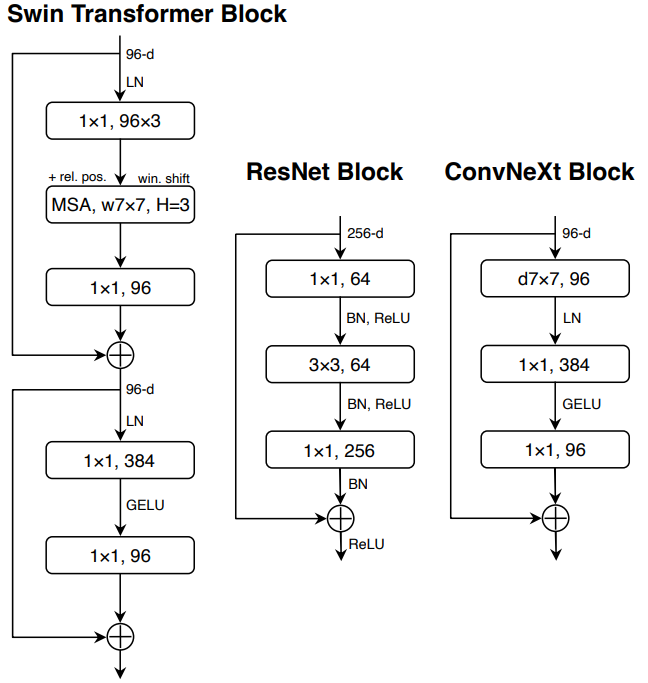
\includegraphics[scale=0.5]{45}
\end{figure}

ConvNeXts enjoy the simplicity of standard ConvNets, but compete favorably with Swin Transformers in visual recognition.
\begin{figure}[H]
	\centering
	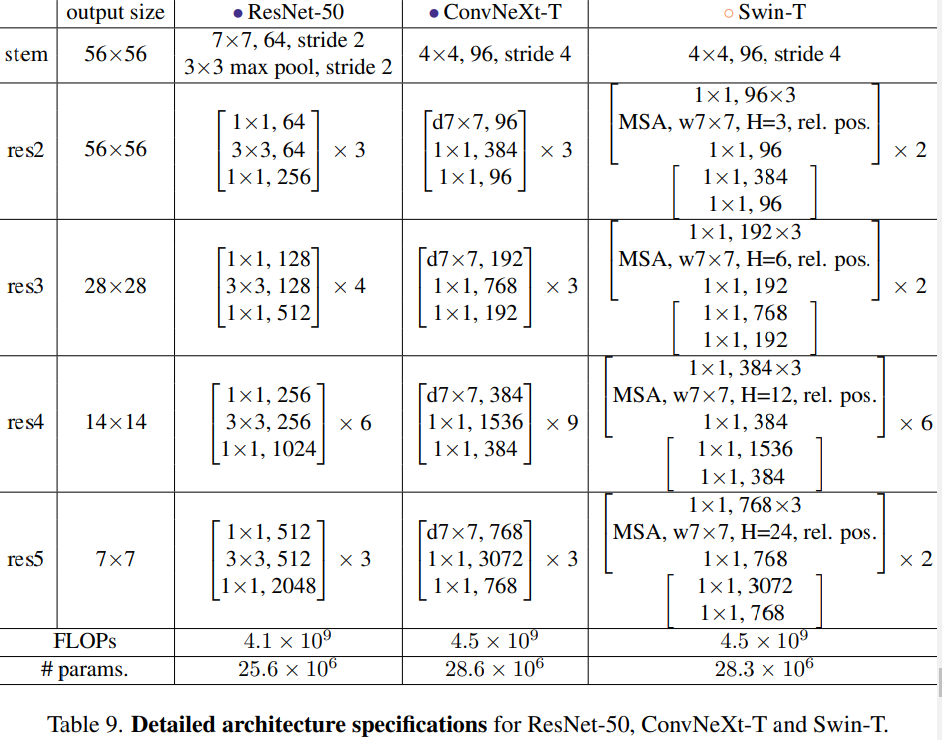
\includegraphics[scale=0.5]{46}
\end{figure}

\subsection{Conclusions}
In the 2020s, vision Transformers, particularly hierarchical ones such as Swin Transformers, began to overtake ConvNets as the favored choice for generic vision backbones. 

The widely held belief is that vision Transformers are moreaccurate, efficient, and scalable than ConvNets. We propose ConvNeXts, a pure ConvNet model that can compete favorably with state-of-the-art hierarchical vision Transformers across multiple computer vision benchmarks, while retaining the simplicity and efficiency of standard ConvNets. 

In some ways, our observations are surprising while our ConvNeXt model itself is not completely new many design choices have all been examined separately over the last decade, but not collectively. We hope that the new results reported in this study will challenge several widely held views and prompt people to rethink the importance of convolution in computer vision.
\section{Multi-Instance Pose Networks: Rethinking Top-Down Pose Estimation}
$\text{https://rawalkhirodkar.github.io/mipnet/}$
\subsection{Abstract}
A key assumption of top-down human pose estimation approaches is their expectation of having a single person/instance present in the input bounding box.This often leads to failures in crowded scenes with occlusions.

We introduce a Multi-Instance Modulation Block (MIMB) that can adaptively modulate channel-wise feature responses for each instance and is parameter efficient.

\subsection{Introduction}
However, when presented with inputs containing multiple humans like crowded or occluded instances, top-down methods are forced to select a single plausible configuration per human detection.

\begin{figure}[h]
	\centering
	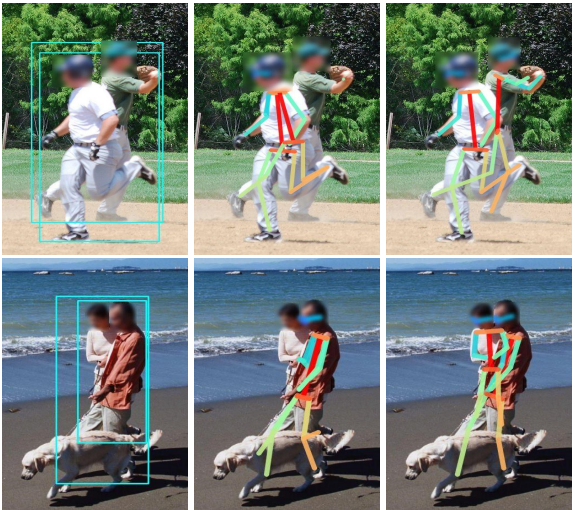
\includegraphics[scale = 0.5]{47}
\end{figure}

The key idea of our proposed architecture is to allow the model to predict more than one pose instance for each bounding box.

A nave approach to predict multiple instances per bounding box would be to add multiple prediction heads to an existing top-down network with a shared feature-extraction backbone.However, such an approach fails to learn different features corresponding to the various instances. 

A brute-force approach would then be to replicate the feature-extraction backbone, though at a cost of an N-fold increase in parameters, for N instances.

In contrast, our approach enables predicting multiple instances for any existing top-down architecture with a small increase in the number of parameters (< 3\%) and inference time (< 9ms, 16\%). Technically, our approach can handle N > 2 instances.

MIMB modulates the feature tensors based on a scalar instance-selector, $\lambda$, and allows the network to index on one of the N instances.MIMB can be incorporated in any existing feature-extraction backbone, with a relatively simple (< 15 lines) code change (refer supplemental).

At inference, for a given bounding box,we vary the instance-selector λ to generate multiple pose predictions.

Many of these bounding boxes overlap and majority have low detection scores (< 0.4). This also adversely impacts the inference time, which increases linearly with
the number of input bounding boxes.

\subsection{Contributions}

1.We advance top-down 2D pose estimation methods by addressing limitations caused by the single person assumption during training and inference.

2.MIPNet allows predicting multiple pose instances for a given bounding box efficiently by modulating feature responses for each instance independently.

3.The ability to predict multiple instances makes MIPNet resilient to bounding box confidence and allows it to deal with missing bounding boxes with minimal impact on performance.

\subsection{Related Work}

\textbf{Biased benchmarks}:

These datasets(OCHuman,CrowdPose) demonstrate the failures of the state-of-art models under severe occlusions.MIPNet shows a significant improvement in performance under such challenging conditions.

\textbf{Occluded pose estimation}:

1.use a top-down models to make a multi-peak prediction and joint peaks are then groupsed into persons using a graph model.

2.use instance segmentation for occlusion reasoning.

3.use a graph neural network to refine pose proposals from a top-down model.

4.use a bottom-up method which uses a differentiable hierarchical graph grouping for joint association.

Instead of training multiple models, our approach enables training a single network for predicting multiple outputs on the same input. Rather than duplicating the feature backbone.

our novel MIMB block leads to a parameter efficient design.Our multi-instance pose network is fully supervised and not related to multiple instance learning, which is a form of weakly-supervised learning paradigm where training instances are arranged in sets.

\subsection{Method}
Human pose estimation aims to detect the locations of K keypoints from an input image x $\in \mathcal{R}^{H\times W\times 3}$.

Most top-down methods transform this problem to estimating K heatmaps, where each heatmap indicates the probability of the corresponding keypoint at any spatial location.

The bounding box at training and inference is scaled to $H\times W$ and is provided as an input to P.

1.Let $\mathcal{y} \in \mathcal{R}^{H'\times W'\times K}$denote the K heatmaps corresponding to the ground truth keypoints for a given input x.

2.The pose eatinator tranforms input x to a single set of predicted heatmaps, $\hat{\mathcal{y}}(\in \mathcal{R}^{H'\times W'\times K}) = P(x)$.

3.P is trained to minimize the mean squared loss $\mathcal{L} = MSE(y,\hat{y})$.
\subsubsection{Training Multi-Instance Pose Network}
Our pose eatimator P predicts N instances. (This is achieved by conditioning the network P on a scalar instance selector $\lambda$,$0\leq \lambda \leq N-1$).

P accepts both x and $\lambda$ as input and predicts $\hat{y_i} = P(x, \lambda=i)$, where $i\in {0,1,...,N-1}$

Let $B_0$ denote the ground truth bounding box used to crop the input x.Let $B_i, i\in {1,...,n-1}$,de note additional n-1 ground truth bounding boxes which overlap $B_0$.(such as at least k=3 keypoints from $B_i$ fall within $B_0$)

Thus $B_0,...,B_{n-1}$ represents the bounding boxes for n ground truth pose instances present in x.We denote the ground truth heatmaps corresponding to these n instances by $y_0,...,y_{n-1}$.

The Loss function:
$$L_i=\left\{\begin{matrix}
	MSE(y_i, P(x,\lambda =i)), \forall 0 \leq i< min(n,N),\\ 
	MSE(y_0, P(x,\lambda =i)), \forall min(n,N)\leq i<N .
\end{matrix}\right.$$

The primary instance $\hat{y_0} = P(x,\lambda=0)$ is assigned to $y_0$.We train the network P to minimize the loss $\mathcal{L} = \frac{1}{N}\sum_{i=0}^{N-1}\mathcal{L}_i$.

When n $\leq$ N, the available m ground truth pose instance are used to compute the loss for n predictions, and the loss for residual N-n instances is computed using $y_0$

\begin{figure}[h]
	\centering
	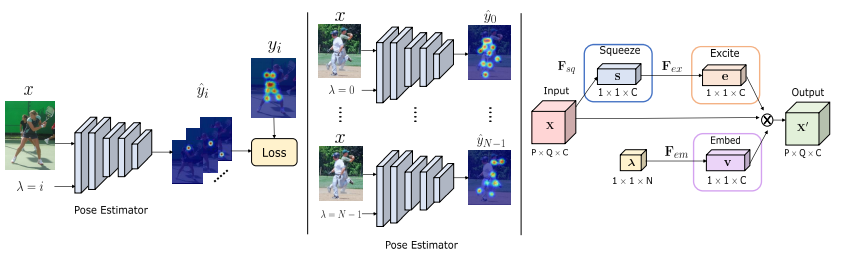
\includegraphics[scale = 0.5]{48}
\end{figure}

During inference, we vary $\lambda$ to extract different pose predictions from the same input x.
\subsection{Conclusion}
Top-down 2D pose estimation methods make the key assumption of a single person within the input bounding box.While these methods have shown impressive results, the single person assumption limits their ability to perform well.in crowded scenes with occlusions.

Our proposed Multi-Instance Pose Network, MIPNet, enables top-down methods to predict multiple instances for a given input. MIPNet is efficient in terms of the number of additional network parameters and is stable with respect to the quality of the input bounding boxes. 

MIPNet achieves state-of-art results on challenging datasets with significant crowding and occlusions. We believe that the concept of predicting multiple instances is an important conceptual change and will inspire a new research direction for top-down methods.
\section{Cascade Feature Aggregation for Human Pose Estimation}
\subsection{Abstract}
Human pose estimation plays an important role in many computer vision tasks and has been studied for 
many decades. However, due to complex appearance variations from poses, illuminations, occlusions and 
low resolutions, it still remains a challenging problem.

Taking the advantage of high-level semantic information from deep convolutional neural networks is an effective way to improve the accuracy of human pose estimation
\subsection{Introduction}
Human pose estimation refers to the task of recognizing postures by localizing body keypoints from 
images.

The typical methods include pictorial structures models, hierarchical models and 
non-tree models

\textbf{1.Pictorial Structures Model:}Constructing a classical tree-structured graphical framework by exploring spatial correlations between parts of the body and kinematic priors that couple connected limbs.

\textbf{2.Hierarchical Models:}Representing the relationships between parts at different scales in a 
hierarchical tree structure, leading to capture high-order relationships among parts and characterize an exponential number of plausible poses.

\textbf{Non-tree Models:}Using loops to augment the tree structure with additional edges, which can well capture symmetry, occlusion and long-range relationships. 

The three typical methods usually degenerate severely under the wild scenario due to complex appearance variations from various poses, different illuminations, partial occlusions, etc.

Moreover, several hourglass networks are stacked to implement a mechanism for repeated bottom-up, top-down inference allowing for reevaluation of initial estimates and features across the whole image.

As an encoder-decoder model, hourglass use a highway to connect the encoder and decoder parts. More detail local information is brought to decoder to improve the performance.

Benifited from the advantages of aggregating features from different stages, our CFA is more robust to poses, illuminations and partial occlusions than others.
\subsection{Contributions}
1.We proposed a novel Cascade Feature Aggregation (CFA) method for robust human pose estimation 
by leveraging features from different stages under a cascade structure.

2.By fusing the results from different stages, CFA can further improve the results for human pose 
estimation.

3.Our CFA outperforms the state-of-the-art methods and achieves the best performance on the MPII 
benchmark.

\subsection{Related Work}
Traditional methods rely on hand-craft features, which formulate the problem of human keypoints estimation as a tree-structured or graphical model problem.

In terms of network architecture(deep convolutional neural network), current human pose estimation methods could be divided into two categories: single-stage approaches and multi-stage approaches.

Generally multi-stage architecture performs better than single-stage methods.

\textbf{Single-Stage Approach:}The most single-stage approaches concentrate on designing the basic network structure.

Hourglass is one of the most typical single-stage approaches. The hourglass considers the information at different scale. High layers have a coherent understanding of the full body, and high way connections bring the essential local evidence to high layers for identifying features like faces and hands.Many researches are devoted to improving the basic network architecture of hourglass.

The first stage endeavors to roughly approximate the body keypoint locations, and therefore an
hourglass is designed for predict the keypoints. After getting an estimation of keypoints from the first stage, the successive hourglasses make an effort to refine the shape by combining the preview prediction and current prediction. Furthermore, the final heat map is averaged by the last few stages for further improving the keypoints predictions.

\textbf{Multi-Stage Approach:}The multi-stage approach focuses on building multiple stages to further
improving the performance.

CPM firstly introduces multi-stage structure with several convolution and pooling layers, which reaches 88.5\% PCKh on MPII test set. CPM illustrates that a sequential architecture composed of convolutional networks is capable of implicitly learning a spatial model for pose by communicating increasingly refined uncertainty-preserving beliefs between stages.

Stack hourglass stacks several hourglass networks to achieve more powerful architecture for human pose estimation.
\subsection{Network Architecture}
\subsubsection{Overview}
\begin{figure}[h]
	\centering
	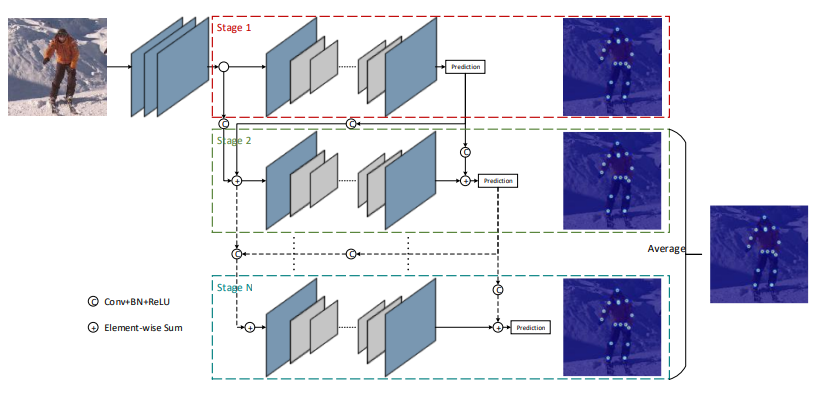
\includegraphics[scale = 0.55]{49}
\end{figure}
Specifically, the CFA framework consists of several successive cascaded hourglass with features aggregations. Each stage attempts to characterize the nonlinear mappings from body image to body keypoints in same feature input transformed from the original image.

Support we have a training set ${(x_i,z_i)}^N_{i=1}$, which consists of N face images $x_i$ and its corresponding p body keypoint $z_i \in R^{2p}$.

We use gaussian kernel to present the p points in an image with p channels,i.e. the heatmaps for p points denoted as $y_i$.

The human pose estimation task can be reformulated as seeking a mapping function $f:y_i =f(x_i)$
\subsubsection{Backbone Model}
\begin{figure}[h]
	\centering
	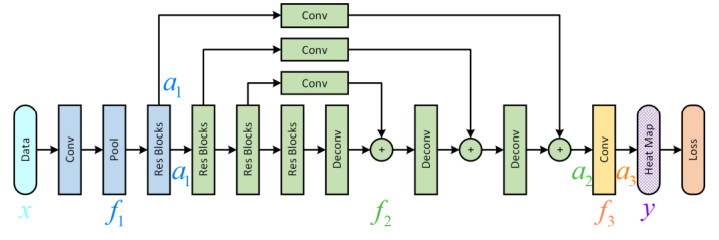
\includegraphics[scale = 0.6]{50}
\end{figure}
Aggregation between different stage of CFA. There are three different aggregation between different stages. The input aggregation brings the local detail information for miss predicted point for a second time prediction. The feature aggregation takes the high layer sematic to input layer. And the 
prediction aggregation keeps the prediction more stable. 

For backbone model, the seeking function $f$ can be expressed as$f(x)=f_3(f_2(f_1(x)))$, where x
is the input image for prediction,$f_1,f_2,f_3$is three parts of the network, and $a_i$ is recorded as 
the result of $f_i$, then we can achieve that $a_1 = f_1(x),a_2 = f_2(a_1), a_3 = f_3(a_2),y=a_3$

Finally we calculate prediction of the keypoints z by $z = g(y)$, g donates the strategy to calculate the keypoint from feature map. In this paper, we treat the coordinate of max value on the heatmap as the prediction function g.
\subsubsection{Cascaded Feature Aggregation}
\begin{figure}[h]
	\centering
	\includegraphics[scale = 0.8]{51}
\end{figure}
Suppose we have a training set ${(x_i.z_i)}^N_{i=1}$, we mapping the ground truth keypoints $z_i$ to the heatmap $y_i^*$ by gaussian function.

We calculate the predicted heatmap of each stage by:
$$y_{i,j}=\left\{\begin{matrix}
	a_{i,j,3} &j=1\\ 
	a_{i,j,3}+\varphi_{j,4}(y_{i,j-1})  &j\geq 2
\end{matrix}\right.$$

Here, j donates the j-th stage. For the first stage, the network output $a_{i,j,3}$is learn to approximate the ground truth heatmap $y_i^*$. For the latter stages, a non-linearity function$\varphi_{j,4}$ is designed by taking the heatmap from previous stage as input and the output from $\varphi_{j,4}$ are further added with $a_{i,j,3}$ to achieve the final heatmap estimation. It can amplify points with high confidents and block the miss predicted points.

We simplify $a_{i,j,3}$ into $a_{j,3}$ for general samples.For each stage, $a_{j,3}$ is calculated by the following funvtion:
$$a_{j,3} = f_{j,3}(f_{j,2}(a_{j,1}))$$

Here $a_{j,1}$ is the input of current stage. $f_{j,2}$ and $f_{j,3}$ has the same struct as $f_2$ and $f_3$ respectively in the backbone model.

For the first stage, $a_(1,1)$ is calculated from the original image:$$a_{1,1} = f_{1,1}(x)$$

For the successive stages,$a_{j,1}$consists of three parts, i.e., low-level features, middle-level features and high-level features from the previous stage.

$$a_{j,1} = \varphi_{j,1}(a_{j-1,1})+\varphi_{j,2}(a_{j-1,2})+\varphi_{j,3}(y_{j-1}) \qquad j\geq2$$

Here$\varphi_{j,1},\varphi_{j,2},\varphi_{j,3}$donate low level, middle level, high level aggregation functions respectively from the preview stage for the inputs of the current stage.

The low-level features contain detailed local information which is beneficial for localizing the exact positions for human parts. While high-level features contain global semantic information, which can improve the performance for partial occlusions and complex backgrounds.

\subsubsection{Results inprovement by fusing heatmaps}
We fuse the heatmaps of the last few stages to further improve the results.
\begin{figure}[h]
	\centering
	\includegraphics[scale = 0.5]{52}
\end{figure}
The prediction is determined by averaging the output heatmaps of last several stages:
$$\sigma_{fusion} = \frac{\sqrt{\sum_{i=N-n}^{N}\sigma_i^2}}{n}$$
where $\sigma_{N-n}...\sigma_N$ denotes the heatmaps of the last N stages. The fusion strategy makes the rasults more stable.
\subsection{Conclusions}
In this paper, we propose a novel method CFA for robust human pose estimation, which cascades 
several hourglasses and aggregates features of low-level, middle-level and high-level to well capture local detailed information and global semantic information. Moreover, the proposed CFA exploits ResNet-101 and ResNet-50 for the first stage and the following stages respectively, which achieves a good trade-off of both accuracy and efficiency.Besides, the experiments results show that the 
data diversity is extremely important for improving performance
\section{Rethinking the Heatmap Regression for Bottom-up Human Pose Estimation}
$\text{https://github.com/greatlog/SWAHR-HumanPose}$
\subsection{Abstract}
Heatmap regression has become the most prevalent choice for nowadays human pose estimation methods.The ground-truth heatmaps are usually constructed via covering all skeletal keypoints by 2D gaussian kernels(the standard deviations of these kernels are fixed).

To better cope with problems(bottom-up methods need to handle a large variance of human scales and labeling ambiguities),we propose the scale-adaptive heatmap regression(SAHR) method, which can adaptively adjust the standard deviation for each keypoint.

We further introduce the weight-adaptive heatmap regression (WAHR) to help balance the fore-background samples.
\subsection{Introduction}
Top-down methods:All persons are firstly cropped out by a human detector and then resized to the same size before they are input to the keypoints detector.

Bottom-up methods:Detecting keypoints of all persons simultaneously. It is more light-weight fast but suffers from various human scales.

The ground-truth heatmaps are constructed by putting 2D Gaussian kernels on all keypoints.

Different keypoints are supervised by the same constructed heatmaps.But we argue that this is unreasonable in two aspects:

1.keypoints of different scales are semantically discriminative in regions of different spatial sizes. It may cause confusion to put the same gaussian kernel on all keypoints

2.humans could not label the keypoints with pixel-wise accuracy, and the ground-truth coordinates may have inherent ambiguities.

Specifically, we firstly cover all keypoints by Gaussian kernels of the same base standard deviation $\sigma_0$. We add a new branch to predict scale maps $s$, which are of the same shape as ground-truth heatmaps. Then we modify the original standard deviation for each keypoint to $\sigma_0\cdot s$ by a point-wise operation. Thus to some extent, s represents the scales and uncertainties of corresponding keypoints.

\subsection{Contributions}
1.This is the first paper that focuses on the problems in heatmap regression when tackling large variance of human scales and labeling ambiguities.

2.We propose a scale-adaptive heatmap regression(SAHR), which can adaptively adjust the standard deviation of the Gaussian kernel for each keypoint, enabling the model to be more tolerant of various human scales and labeling ambiguities.

3.We propose a weight-adaptive heatmap regression(WAHR) to alleviate the severe imbalance between foreground and background samples. It could automatically focus more on relatively harder examples and fully exploit the superiority of SAHR.
\subsection{Related Works}
\subsubsection{Bottom-up Human Pose Estimation}
Bottom-up(usually inferior on accuracy) HPE methods firstly detect all identity-free keypoints and then group them into individual persons.

Bottom-up methods have to tackle the grouping problem and large variance of human scales.

Recent works about bottom-up HPE mostly focus on developing better grouping methods.

Although the grouping method has been advanced a lot, few works are done about the various human scales. So we mainly focus on the problems in bottom-up HPE when tackling large variance of human scales.
\subsubsection{Heatmap Regression}
Heatmap regression is widely used for semantic landmarks localization.

The ground-truth heatmaps are construced by putting 2D Gaussian kernels on the labeled points.

The pixel values on the heatmaps are usually treated as the probabilities of corresponding pixels being the keypoints.

However, current methods typically cover all keypoints by Gaussian kernels with the same standard deviations.

It may work well for top-down methods,in which all persons are resized to the same size.

But in bottom-up methods, in which persons are of various scales,it seems to be more desirable to adjust the standard deviation for each keypoint according to the scale of the corresponding person.

\subsubsection{Uncertainly Prediction}
As there are usually inevitable labeling ambiguities in the training datasets, it is better to explicitly model the uncertainty for predivtions.

Original heatmap regression covers keypoints by Gaussian kernels while keeping standard deviations fixed.In that case, the ambiguities of different keypoints are assumed to be the same. This implicit assumption may be too strong and potentially hurt the performance.

In this paper, the scale-adaptive heatmap regression alleviates this problem by introducing scale maps to adaptively modify the standard deviation for each keypoint.

\subsection{Proposed Method}
\subsubsection{Formulation}
Suppose $C^p_k={x^p_k,y^p_k}$ denotes the coordinate of the $k^{th}$ keypoint of the $p^{th}$ person.

$h^p$ denotes its corresponding ground-truth heatmap, then th ecovered region for $C_k^p$ is written as:
$$h^p_{k,i,j}=\left\{\begin{matrix}
	e^{-\frac{((i-x_k^p)^2+(j-y_k^p)^2)}{2\sigma^2}} &s.t. \left \| i-x^p_k\right \|_1\leq 3\sigma \qquad s.t. \left \| j-y^p_k\right \|_1\leq 3\sigma \\ 
	0 &s.t. \left \| i-x^p_k\right \|_1>3\sigma \qquad s.t. \left \| j-y^p_k\right \|_1>3\sigma 
\end{matrix}\right.$$

If the number of persons is N, then the overall ground-truth heatmaps are $$H^{\sigma}=max \{h^1,h^2,...,h^N\}$$
where $max$ is pixel-wisely operated.

Suppose the predicted heatmaps are P, then the regression loss is 
$$L_{regression}=\left \|P-H^{\sigma} \right \|^2_2$$

\subsubsection{Scale-Adaptive Heatmap Regression}
In previous methods, the standard deviation $\sigma$ is fixed as $\sigma_0$ for all keypoints.Since it is hard to manually label each keypoint, we hope that the model could learn to adjust $\sigma$ by itself.

We add a new branch to predict the scale maps $s$, which are of the shape with ground-truth heatmaps.

For $C^p_k={x^p_k,y^p_k}$, we modify the standard deviation to $\sigma_0\cdot s_{k,x^p_k,y^p_k}$.then the covered region for $C^p_k$ becomes:
$$h^p_{k,i,j}=
	e^{-\frac{((i-x_k^p)^2+(j-y_k^p)^2)}{2(\sigma_0\cdot s_{k,x^p_k,y^p_k})^2}} \qquad s.t. \left \| i-x^p_k\right \|_1\leq 3\sigma \qquad s.t. \left \| j-y^p_k\right \|_1\leq 3\sigma 
$$
Since the civered region is relatively small, we may have $s_{k,x^p_k,y^p_k}\approx s_{k,i,j}$.Thus the modification can be written as an element-wise operation:
$$h^p_{k,i,j}=
e^{-\frac{((i-x_k^p)^2+(j-y_k^p)^2)}{2(\sigma_0\cdot s_{k,i,j})^2}} \qquad s.t. \left \| i-x^p_k\right \|_1\leq 3\sigma \qquad s.t. \left \| j-y^p_k\right \|_1\leq 3\sigma 
$$
We denote the modified heatmaps as $H^{\sigma_0\cdot s}$(we call scale-adaptive heatmaps).If we express $H^{\sigma_0\cdot s}$ by original heatmaps $H^{\sigma_0}$:
$$H^{\sigma_0\cdot s}_{k,i,j}=\left\{\begin{matrix}
(H^{\sigma_0}_{k,i,j})^{1/s_{k,i,j}} &H^{\sigma_0}_{k,i,j}>0\\ 
	H^{\sigma_0}_{k,i,j}&H^{\sigma_0}_{k,i,j}=0 
\end{matrix}\right.$$

For keypoints whose scale factors are larger than 1, their corresponding standard deviation will be larger than $\sigma_0$, which means that the region covered by this Gaussian kernel will also become larger. Otherwise the reverse.

Furthermore, some changes need to be made to stabilize the training:

\noindent1.We add a regularizer loss for the predicted scale maps:$$L_{regularizer}=\left \|(1/s-1)l_{H^{\sigma_0/s>0}} \right \|^2_2$$
$l_{H^{\sigma_0\cdot s>0}}$denotes the mask that keeps only regions covered by gaussian kernels.

\noindent2.We transform the exponential form of $H^{\sigma_0\cdot s}$ into a polynomial series by Taylor expansion at s=1.We omit terms higher than the seconde order:$$H^{\sigma_0\cdot s}_{k,i,j}=\left\{\begin{matrix}
	\frac{1}{2}H^{\sigma_0}_{k,i,j}(1+(1+\alpha_{k,i,j}ln(H^{\sigma_0}_{k,i,j}))^2) &H^{\sigma_0}_{k,i,j}>0\\ 
	0 &H^{\sigma_0}_{k,i,j}=0 
\end{matrix}\right.$$
where $\alpha = 1/s-1$.

Then the total loss is written as:
$$\mathcal{L}_{total}=L_{regression}+\lambda L_{regularizer}=\left \|P-H^{\sigma_0\cdot s>0} \right \|^2_2+\lambda\left \|\alpha l_{H^{\sigma_0/s}>0} \right \|^2_2$$
where $\lambda$ is the weight for regularizer term.In practice, we use $\lambda = 1$.This is what we call scale-adaptive heatmap regression(SAHR)
\subsubsection{Relation to Uncertainty Presiction}
There are inherent labeling ambiguities of box coordinates in some cases.Thus they treat both the predicted and ground-truth coordinates as Gaussian distributions, and the standard deviztions could represent the uncertainties of the coordinates.

The loss is constructed as KL loss:$$\mathcal{L}\propto \frac{\left \|X_p-X_g \right \|^2_2}{2\sigma^2} + \frac{1}{2}log(\sigma^2)$$
where $X_p$ and $X_g$ denote the predicted and ground-truth coordinates respectively. And $\sigma$ is predicted by the model,denotes the standard deviztions of assumed Gaussian Distributions.

We still use L2 loss in SAHR. But instead of keeping the standard deviations fixed, we add a regularizer term to help lead the model to converge to the desired direction.SAHR combines the merits of both heatmap and coordinate regression.

\subsubsection{weight-Adaptive Heatmap Regression}
We experimentally find that SAHR may aggravate the imbalance between fore-background samples in heatmap regression. This imbalance may restrict the improvement of SAHR.
$$\mathcal{L}_{regression} = W\cdot \left \|P-H \right \|^2_2$$
and W can be defined as $$W_{k,i,j}=\left\{\begin{matrix}
	(1-P_{k,i,j}) &\qquad\text{\{k,i,j\} is positive sample} \\ 
	P_{k,i,j}&\qquad\text{\{k,i,j\} is negative sample}
\end{matrix}\right.$$

Towards this issue, we propose a weight-adaptive heatmap regression (WAHR), in which the loss weights are written as:
$$W = (H)^\gamma \cdot \left \|1-P \right \|+\left \|P \right \|\cdot (1-(H)^\gamma)$$
where $\gamma$ is the hyper-parameter that controls the position of a soft boundary.

We can get the soft boundary is defined as a threshoid heatmap values $p=2^{-\frac{1}{\gamma}}$.In practice, we use $\gamma = 0.01$

For samples with heatmap values larger than $p$,their loss weights are more close to $(1-P)$,otherwise sre more close to $P$.
\begin{figure}[H]
	\centering
	\includegraphics[scale = 0.55]{53}
\end{figure}
\subsection{Conclusion}
In this paper, we mainly focus on the problems in heatmap regression when tackling various human scales and labeling ambiguities. We propose a scale-adaptive heatmap
regression (SAHR), which can learn to adjust the standard deviation for each keypoint by itself. Without extra supervision, experiments show that the model could learn the relation between standard deviation and the corresponding human scales. Also, as SAHR may aggravate the imbalance between fore-background samples, we propose a weight-adaptive heatmap regression (WAHR) to alleviate this problem. WAHR could automatically down-weight the loss of well-classified samples and focus more on relatively harder (usually foreground) samples.
\section{MixConv: Mixed Depthwise Convolutional Kernels}
$\text{https://github.com/tensorflow/tpu/tree/master/models/official/mnasnet/mixnet}$
\subsection{Abstract}
Depthwise convolution is becoming increasingly popular in modern efficient ConvNets, but its kernel size is often overlooked.

In this paper, we systematically study the impact of different kernel sizes, and observe that combining the benefits of multiple kernel sizes can lead to better accuracy and efficiency. Based on this observation, we propose a new mixed depthwise convolution (MixConv), which naturally mixes up multiple kernel sizes in a single convolution.
\subsection{Introdution}
Convolutional neural networks (ConvNets) have been widely used in image classification,
detection, segmentation, and many other applications.

Unlike regular convolution, depthwise convolutional kernels are applied to each individual channel separately, thus reducing the computational cost by a factor of C, where C is the number of channels.
\begin{figure}[H]
	\centering
	\includegraphics[scale = 0.55]{54}
\end{figure}
As expected, larger kernel sizes significantly increase the model size with more parameters; however, model accuracy first goes up from 3x3 to 7x7, but then drops down quickly when the kernel size is larger than 9x9, suggesting very large kernel sizes can potentially hurt both accuracy and efficiency

\begin{figure}[H]
	\centering
	\includegraphics[scale = 0.55]{55}
\end{figure}
Mixed depthwise convolution(MixConv)-Unlike vanilla depthwise convolution that applies a single kernel to all channels,MixConv partitions channels into groups and apply different kernel size to each group.
\subsection{Related Work}
\textbf{Efficient ConvNets:}In particular depthwise convolution has been increasing popular in all mobile-size ConvNets.

Unlike regular convolution, depthwise convolution performs convolutional kernels for each channel separately, thus reducing parameter size and computational cost.Our proposed MixConv generalizes the concept of depthwise convolution, and can be considered as a drop-in replacement of vanilla depthwise convolution.

\textbf{Multi-Scale Networks and Features:}By using multiplr branches in each layer, these ConvNets are able to utilize diffierent operations(such as convolution and pooling) in a single layer.

However, unlike these prior works that mostly focus on changing the macro-architecture of neural networks in order to utilize different convolutional ops, our work aims to design a drop-in replacement of a single depth-wise convolution, with the goal of easily utilizing different kernel sizes without changing the network structure.

\textbf{Neural Architecture Search:}Recently, neural architecture search has achieved better performance than hand-crafted models by automating the design process and
learning better design choices.
\subsection{MixConv}
The main idea of MixConv is to mix up multiple kernels with different sizes in a single
depthwise convolution opration, such that it can easily capture different types of patterns from input images.

\subsubsection{MixConv Feature Map}
Let $X^{(h,w,c)}$ denotes the imput tensor with shape (h,w,c), where h is the spatial height,w is the spatial width, and c is the channel size.

Let $W^{(k,k,c,m)}$ denotes a depthwise convolutional kernel, where $k\times k$is the kernel size, c is the input channel size, and m is the channel multiplier. 

The output tensor $Y^{(h,w,c\cdot m)}$ would have the same spatial shape($h,w$) and multiplied output channel size $m\cdot c$, with each output feature map value calculated as:
$$Y_{x,y,z} = \sum_{-\frac{k}{2}\leq i \leq \frac{k}{2},-\frac{k}{2}\leq j \leq \frac{k}{2}}X_{x+i,y+i,z/m}\cdot W_{i,j,z} \qquad \forall z=1,...,m\cdot c$$

More concretely, the input tensor is partitioned into $g$ groups of virtual tensor $<\hat{X}^{(h,w,c_1),...,\hat{X}^{(h,w,c_g)}}$,where all virtual tensors $\hat{X}$ have the same spatial height h and width w, and their total channel size is equal to the original input tensor:$c_1+c_2+...+c_g=c$.

We also partition the convolutional kernel into $g$ groups of virtual kernels $<\hat{W}^{(k_1,k_1,c_1,m),...,\hat{W}^{(k_g,k_g,c_g,m)}}>$.

For $t$-th group of virtual input tensor and kernel, the corresponding virtual output is calculated as:
$$\hat{Y}_{x,y,z}^t = \sum_{-\frac{k_t}{2}\leq i \leq \frac{k_t}{2},-\frac{k_t}{2}\leq j \leq \frac{k_t}{2}}\hat{X}^t_{x+i,y+i,z/m}\cdot \hat{W}^t_{i,j,z} \qquad \forall z=1,...,m\cdot c_t$$

The final output tensor is a concatenation of all virtual output tensor $<\hat{Y}^1_{x,y,z_1},...,\hat{Y}^g_{x,y,z_g}>$:
$$Y_{x,y,z_o} = Concat(\hat{Y}^1_{x,y,z_1},...,\hat{Y}^g_{x,y,z_g})$$
where $z_o = z_1+z_2+...+z_g = m\cdot c$ is the final output channel size.

\subsubsection{MixConv Design Choice}
\textbf{Group Size $g$:} It determines how many different type of kernels to use for a single input tensor.In the extreme case of $g=1$,a MixConv becomes equivalent to a vanilla depthwise convolution.

In our experiments, we find g = 4 is generally a safe choice for MobileNets, but with the help of neural architecture search, we find it can further benefit the model efficiency and accuracy with a variety of group sizes from 1 to 5.

\textbf{Kernel Size Per Group:}We set group $i$ always has kernel size $2i+1$.With this restriction, the kernel size for each group is predifined for any group size $g$, thus simplifying our design process.

\textbf{Channel Size Per Group:}(1)Equal partition:each group will have the same number of filters.(2)Exponential partition:the $i-th$ group will have about $2^{-i}$ portion of total channels.

For example, given a 4-group MixConv with total filter size 32, the equal partition will divide the channels into (8,8,8,8), while the exponential partition will divide the channels into (16,8,4,4)

\textbf{Dilated Convolution:}Since large kernels need more parameters and computations, an alternative is to use dilated convolution, which can increase receptive field without extra parameters and computations.

\subsubsection{Ablation Study}
\textbf{MixConv for Single Layer:}We replace one of the 15 layers with either (1)vanilla DepthwiseConv9x9 with kernel size $9\times 9$;(2)MixConv3579 with 4 groups of kernels:{3x3, 5x5, 7x7, 9x9}.
\begin{figure}[H]
	\centering
	\includegraphics[scale = 0.55]{56}
\end{figure}
s2 denotes stride 2,while others have stride 1.Our MixConv achieves similar or slightly better performance for most of the layers(for the certain layers with stride 2)

\textbf{Channel Partition Methods:}As expected, exponential partition requires less parameters and FLOPS for the same kernel size, by assigning more channels to smaller kernels.

\begin{figure}[H]
	\centering
	\includegraphics[scale = 0.55]{57}
\end{figure}
Performance of exponential partition(+exp) and dilated kernels(+dilated)

\textbf{Dilated Convolution:}For kernel size KxK, it uses a 3x3 kernel with dilation rate
(K −1)/2: for example, a 9x9 kernel will be replaced by a 3x3 kernel with dilation rate 4.We only use dilated convolutions for a layer if its stride is 1.

As shown in the figure, dilated convolution has reasonable performance for small kernels, but the accuracy drops quickly for large kernels. Our hypothesis is that when dilation rate is big for large kernels, a dilated convolution will skip a lot of local information, which would hurt the accuracy.
\subsection{MixNet}
To further demonstrate the effectiveness of MixConv, we leverage recent progress in neural architecture search to develop a new family of MixConv-based models, named as MixNets.
\begin{figure}[H]
	\centering
	\includegraphics[scale = 0.5]{58}
\end{figure}
\subsection{Conclusions}
In this paper, we revisit the impact of kernel size for depthwise convolution, and identify that traditional depthwise convolution suffers from the limitations of single kernel size. To address this issue, we proposes MixConv, which mixes multiple kernels in a single op to take advantage of different kernel sizes. We show that our MixConv is a simple drop-in replacement of vanilla depthwise convolution, and improves the accuracy and efficiency for MobileNets, on both image classification and object detection tasks. Based on our proposed MixConv, we further develop a new family of MixNets using neural architecture search techniques. Experimental results show that our MixNets achieve significantly better accuracy and efficiency than all latest mobile ConvNets on both ImageNet classification and four widely used transfer learning datasets.
\section{Toward fast and accurate human pose estimation via soft-gated skip connections}
$\text{https://github.com/salinasJJ/BBpose}$
\subsection{Abstract}
This paper is on highly accurate and highly efficient human pose estimation.

While residual connections within FCNs(Fully Convolutional Networks) have proved to be quintessential for achieving high accuracy, we re-analyze this design choice in the context of improving both the accuracy and the efficiency over the state-of-the-art.

\subsection{Contributions}
1.We propose gated skip connections with per-channel learnable parameters to control the data flow for each channel within the module within the macro-module.This has the simple effect to learn how much information from the previous stage is propagated into the next one per channel and encourages each module learn more complicated functions

2.We introduce a hybrid network that combines the HourGlass and U-Net architectures
which minimizes the number of identity connections within the network and increases the performance for the same parameter budget.

\subsection{Introdution}
From a practical perspective, many applications can not fully enjoy the high accuracy demonstrated by recent advances.

The reason is for this is two fold:1.the bulk of current work assumes the abundance of computational resources(e.g. GPUs,memory,power) to run these models which for many applications are not available.2.In many application domains(e.g. autonomous driving)accuracy is absolutely essential, and there is very little room for accuracy drop.

Besides being challenging, the problem of human pose estimation under low memory and computing capacity has received little attention from the research community so far.

Our work improves upon these two works by looking into a component of the network architecture(skip connections)
\subsection{Related Work}
\subsubsection{Efficient Neural Nerworks}
Reaching the remarkable levels of performance attained on a variety of tasks bases on powerful computational resource, large amount of annotated data, architectural improvements.

Deeper neural networks makes for harder to train networks:1.incease in the number os parameters 2.gradient vanishing or exploding.

U-Nets by introducing skip connections between the encoder and decoder parts.

DenseNet proposes to introduce one to all connections between a convolutional block and its successors within the same block.

MobileNet builds on the same principle but explicitly parametrizes the convolutions as separable ones (e.g. their kernels can be expressed as the sum of rank one tensors).

The authors propose to leverage 1 × 1 convolutions and skip connections to achieve performance similar to AlexNet on ImageNet but with a fraction of the parameters.

\subsubsection{Human Pose Estimation}
Both HourGlass and U-Net architectures consist of a stack of encoder-decoder Fully Convolutional Networks with skip connections between the encoder and the decoder part.

\begin{figure}[H]
	\centering
	\includegraphics[scale = 0.5]{59}
\end{figure}

In <Efficient object localization using convolutional networks>, the authors propose a coarse-to-fine learning mechanism where an initial coarse prediction is refined at a later stage by zooming-in into a region of interest and predicting a correction (expressed as an offset from the coarse detection).

The work of<Human pose estimation using deep consensus voting> proposes to localize the landmarks using a dense voting technique where joint probabilities are learned from relative keypoint locations.

In <Recurrent human pose estimation> , the authors introduce a hybrid architecture that combines a normal feed-forward model with a recurrent block.

In a similar spirit with <Stacked hourglass networks for human pose estimation>,<Convolutional pose machines> propose a 6-stack neural network to detect and gradually refine the keypoint predictions.

In <Human pose estimation via convolutional part heatmap regression> the authors attempt to improve the localization process by diving the keypoint detection task into two sup-problems: detection and regression. At the first stage they detect only the visible landmarks using a part detection network, while at the second one they regress jointly the position of all keypoints, both visible and occluded.

More recent mothods attempt to combine the HG based architecture with attention mechanisms,feature pyramids and adversarial training.

The work of <Multi-context attention for human pose estimation> uses a Conditional Random Field in order to model the correlations among nearby regions combining a holistic attention model with a body part one. This way the network learns to focus on both global and local details.

In order to enforce a stronger model, in <Self adversarial training for human pose estimation>, the authors propose an adversarial training approach where the pose estimator has the role of a generator. At training time a discriminator is used to assess the quality of the produced heatmaps.

A similar approach is followed in <Adversarial training for human pose estimation>, where a discriminator is used to discern between feasible and biologically unfeasible poses.

<Learning feature pyramids for human pose estimation> proposes a Pyramid Residual Module to improve the scale invariance of the models. The Pyramid Residual Module learns a series of convolutional filters at various input scales, on features obtained using different sub-sampling ratios.

In <Multi-scale structure-aware network for human pose estimation>, the authors propose a series of architectural enhancements aimed at improving the overall network robustness such as the addition of a multi-scale supervision, a structure-aware loss and a keypoint masking technique aimed at increasing the accuracy of the occluded points.

With the goal of strengthening the intrinsic human body model learned by the network, <Deeply learned compositional models for human pose estimation> introduces a compositional model that learns the relation between various
body parts.

To our knowledge, the only papers that have similar aims with our work are <Binarized convolutional lanmark localizers for human pose estimation and face alignment with limited resource> and <Cu-net: Coupled u-nets>.The former one proposes to improve the speed of human pose estimation by fully binarizing the features and the weights of a given network. The work of the latter one combines dense connections with the HG model improving the overall accuracy and speed.

\subsection{Method}
\subsubsection{Soft-gated Residual Connections}
Residual connections have since become a ubiquitous part of current state-of-the-art neural network architectures and are often considered a quintessential aspect that drives their accuracy. Despite this, we argue here that, at least for some cases, the presence of an identity connection may have undesirable effects and hinder the performance of the model.

In the quest for training very deep neural networks, the effect of using a hard gating function $g(x)=\sigma(W_gx+b_g)$,where $\sigma$ is the sigmoid function,$w_g$ and $b_g$ the weights and respectively the bias of a given hard gating transformations.Typically
$g(x)$ is implemented using a convolutional layer with a kernel size of 1×1.

Since in an HourGlass stack, typically, at each resolution level inside the encoder
and decoder a very small number of residual blocks are used (usually one), forcing the blocks to learn a correction with respect to the input hinders the learning process and goes against the finding from [16] that suggest that at the transition level between resolutions novel functions need to be learned by the network.

In this work, we propose a novel way of improving the residual module using a channel-wise soft gating mechanism defined as bellow:
$$x_{l+1} = \alpha x_l + \mathcal{F}(x_l,W_l)$$
where $x_l\in \mathcal{R}^{C\times w\times h}$ are the input features from the previous layer, $W_l$ is a set of weights associated with the $l$th residual block and $\mathcal{F}$ a residual function implemented using a set of convolutional layers.$\alpha\in \mathcal{R}^{C\times 1}$ is a channel-wise soft gate(scaling factor) thst is learned via backpropagation.

\begin{figure}[H]
	\centering
	\includegraphics[scale = 0.5]{60}
\end{figure}

In the process we explore two different settings:1.using a single soft gate for all channels.2.learning a value for each input channel.

\begin{figure}[H]
	\centering
	\includegraphics[scale = 0.5]{61}
\end{figure}
PCKh-based comparison with state-of-the-art on the MPII validation set for different values and methods of computing the scaling factor $\alpha$

\begin{figure}[H]
	\centering
	\includegraphics[scale = 0.5]{62}
\end{figure}
Interestingly, we notice that the majority of the values are clustered around
0, which means that most of the information is not needed, or potentially even harmful for training. This phenomenon is observed across all layers of the network, regardless of
the depth.(it is not essential for the $x_l$)

Notice that most of the features coming from the previous block are filtered by the introduced channel-wise scaling factor.The scaling factors allows the module to select only the useful information from the previous stage.

\subsubsection{Improved Network Architecture}
\begin{figure}[H]
	\centering
	\includegraphics[scale = 0.4]{63}
\end{figure}
(Base)The features coming from the encoder are merged in the decoder using element-wise summation, resulting in the same dimensionality N.
\begin{figure}[H]
	\centering
	\includegraphics[scale = 0.4]{64}
\end{figure}
The features are first concatenated; a convolutional layer with a $3\times 3$ kernel then reduces their dimensionality back to N.
\begin{figure}[H]
	\centering
	\includegraphics[scale = 0.4]{65}
\end{figure}
The features are concatenated and then processed using a grouped convolutional layer with a kernel of size $3\times 3$
\subsection{Conclution}
In this paper, we revisited residual units and introduceda new learnable soft gated skip connections. Specifically, our proposed block has gated per-channel skip connections, where each channel has a learnable parameter that controls the data flow between the current and previous residual module. In addition, we introduce a hybrid network that combines the HG and U-Net architectures which minimizes the number of identity connections within the network and increases the performance for the same parameter budget. We demonstrate superior performance and efficiency on the challenging task of human body-pose estimation. Specifically, our model obtains state-of-the-art results on the MPII and LSP datasets. In addition, with a reduction of 65\% in model size and complexity, we show no decrease in performance when compared to the original HG network.
\section{GhostNet: More Features from Cheap Operations}
$\text{https://github.com/huawei-noah/CV-Backbones}$
\subsection{Abstract}
Deploying convolutinal neural networks(CNNs) on embedded devices is difficult due to the limited memory and computation resources.

This paper proposes a novel Ghost module to generate more feature maps from cheap operations.

Based on a set of intrinsic feature maps, we apply a series of linear transformations with cheap cost to generate many ghost feature maps that could fully reveal information underlying intrinsic features.

The proposed Ghost module can be taken as a plug-and-play component to upgrade existing convolutional neural networks.

\subsection{Introdution}
Traditional CNNs usually need a large number of parameters and floating point operations(FLOPs) to achieve a satisfactory accuracy.

Abundant and even redundant information in the feature maps of well-trained deep neural networks often guarantees a comprehensive understanding of the input data.

Presenting some feature maps of an input image generated by ResNet-50, and there exist many similar pairs of feature maps.Instead of avoiding the redundant feature maps, we tend to embrace them, but in a cost-efficient way.

An ordinary convolutional layer in deep neural networks will be split into two parts:

\noindent1.Ordinary convolutions but their total number will be rigorouly controlled.
\noindent2.Given the intrinsic feature maps from the first part, a series of simple linear operations are then applied for generating more feature maps.

Without changing the size of output feature map, the overall required number of parameters and computational complexities in this Ghost module have been decreased, compared with those in vanilla convolutional neural networks.
\subsection{Related Work}
\subsubsection{Model Compression}
Model compression aims to reduce the computation, energy and storage cost.

Pruning connections cuts out the unimportant connections between neurons.

Channel pruning further targets on removing useless channels for easier acceleration in practice.

Model quantization represents weights or activations in neural networks with discrete values for compression and calculation acceleration.

Binarization methods with only 1-bit values can extremely accelerate the model by efficient binary operations.

Tensor decomposition reduces the parameters or computation by exploiting the redundancy and low-rank property in weights.

Knowledge distillation utilizes larger models to teach smaller ones, which improves the performance of smaller models.
\subsubsection{Compact Model Design}
Xception utilizes depthwise convolution operation for more efficient use of model parameters.

MobileNets are a series of light weight deep neural networks based on depthwise separable convolutions.

MobileNetV2 proposes inverted residual block and MobileNetV3 further utilizes AutoML technology achiecing better performance with fewer FLOPs.

ShuffleNet introduces channel shuffle oparetion to improve the information flow exchange between channel groups.

ShuffleNetV2 further considers the actual speed on target hardwera for compact model design.

Pointwise convolutions process features across channels.Depthwise convolutions processs spatial information.
\subsection{Convolutions}
\noindent1.The primary convolution in Ghost module can have customized kernel size.

\noindent2.Ghost module adopts ordinary convolution to first generate a few intrisic feature maps, and then utilizes cheap linear operations to augment the features and increase the channels.

\noindent3.The identity mapping is paralleled with linear transformations in Ghost module to preserve the intrinsic feature maps.

\noindent4.Ghost module can have large diversity.
\subsection{Approach}
\subsubsection{Ghost Module for More Features}
Given the widely existing redundancy in intermediate feature maps calculated by mainstream CNNs.

In pratice, given the input data $X\in \mathcal{R}^{c\times h\times}$, where c is the number of input channels and $h$ and $w$ are the height and width of the input data, respectively the opration of an arbitrary convolutional layer for producing $n$ feature maps can be formulated as 
$$Y = X*f +f$$
where $*$ is the convolution opration, $b$ is the bias term, $Y\in \mathcal{R}^{h'\times w'\times n}$ is the output feature map with $n$ channels, and $f\in \mathcal{R}^{c\times k\times k\times n}$ is the convolution filters in this layer.

In addition, $h'$ and $w'$ are the height and width of the output data, and $k\times k$ is the kernel size of convolution filters $f$.

During the convolution procedure, the required number of FLOPs can be calculated as $n\cdot h'\cdot w'\cdot c\cdot k\cdot k$, which is often as large as hundreds  of thousands since the number of filters $n$ and the channel number $c$ are generally very large(e.g. 256 or 512)

\begin{figure}[H]
	\centering
	\includegraphics[scale = 0.5]{66}
\end{figure}

We point out that it is unnecessary to generate these redundant feature maps one by one with large number of FLOPs and parameters.

These intrinsic feature maps are often of smaller size and produced by ordinary convolution filters.

Specifically, $m$ intrinsic feature maps $Y'\in\mathcal{R}^{h'\times w'\times m}$ are generated using a primary convolution:
$$Y' = X*f'$$
where $f'\in \mathcal{R}^{c\times k\times k\times m}$ is the utilized filters, $m\leq n$ and the bias term is omitted for simplicity.

\begin{figure}[H]
	\centering
	\includegraphics[scale = 0.5]{67}
\end{figure}

To further obtain the desired n feature maps, we propose to apply a series of cheap linear operations on each intrinsic feature in $Y'$ to generate $s$ ghost feature according to the following function:

$$y_{ij}=\phi_{i,j}(y'_i), \forall i=1,...,m,  \quad j=1,...,s,$$
where $y'_i$ is the i-th intrinsic feature map in $Y'$, $\phi_{i,j}$ in the above function is the j-th(except the last one)linear opration for generating the j-th ghost feature map $y_{i,j}$

The last $\phi_{i,s}$ is the identity mapping for preserving the intrinsic feature maps.We can obtain $n=m\cdot s$ feature maps$Y=[y_{11},y_{12},...,y_{ms}]$ as the output data of a Ghost module.

In practice, there could be several different linear operations in a Ghost module, e.g.
$3\times 3$ and $5\times 5$ linear kernels, which will be analyzed in the experiment part.
\subsection{Building Efficient CNNs}
The Ghost bottleneck appears to be similar to the basic residual block in ResNet in which several convolutional layers and short-cuts are integrated.
\begin{figure}[H]
	\centering
	\includegraphics[scale = 0.5]{68}
\end{figure}
The first Ghost module acts as an expansion layer increasing the number of channels. We refer the ratio between the number of the output channels and that of the input as expansion ratio.

The second Ghost module reduces the number of channels to match the shortcut path.

Then the shortcut is connected between the inputs and the outputs of these two Ghost modules.
\subsection{Conclusion}
To reduce the computational costs of recent deep neural networks, this paper presents a novel Ghost module for building efficient neural architectures. The basic Ghost module
splits the original convolutional layer into two parts and utilizes fewer filters to generate several intrinsic feature maps. Then, a certain number of cheap transformation operations will be further applied for generating ghost feature maps efficiently. The experiments conducted on benchmark models and datasets illustrate that the proposed method is a plug-and-play module for converting original models to compact ones while remaining the comparable performance. In addition, the GhostNet built using the proposed new module outperforms state-of-the-art portable neural architectures, in both terms of efficiency and accuracy.
\section{AID: Pushing the performance boundary of human pose estimation with information dropping augmentation}
\subsection{Abstract}
There is a tendency in most existing works to overfitting the formar and overlook the latter.

In this paper, we propose AID(Augmentation by Information Dropping) to verify and trackle this dilemma.

We hope AID to be a regular configuration for training human pose estimators.
\subsection{Introduction}
Human pose estimation serves many visual understanding tasks such as video surveillance and action recognition.

Witing a significant advance from single person to multi-person pose estimation.The key engine consists of the network architecture evolution, unbiased data processing and effective grouping strategies.

Some overfitting problem is a conjecture raised in rethinking the relationship between manually labeling methods and the model training supervisions.

The base information that human use for keypoint locating is the appearance cues and this inspires the pioneers to use response map.

Besides, another cue is the constraints like the keypoint relationship in human pose or the interaction between human and its surrounding environment.The appearance cue is intuitively easier for acquiring with convolutional neural network.

When the appearance cue is always present and there are no penalty on the neglecting of constraint cue, we suspect that the algorithms only with response map supervision have a tendency to overfitting the appearance cue.

By dropping information in images, the neural networks can learn discriminative features, resulting in a notable increase of model robustness.

Inspired by this, we randomly drop the appearance information of a keypoint and maintain the response map supervision, in purpose of preventing the trained estimators from overfitting the appearance cues and making it pay more attention to the constraints.

Specifically, the appearance information shortage caused by AID challenges the early training process, confusing the network.To address this problem, two customized training schedules are proposed in this paper to provide the prerequisite access for
higher performance human pose estimation with AID.

\subsection{Contributions}
We summarize two discoveries here: 
\noindent(a) Performance of different information dropping methods is various in bottom-up paradigm while is close in top-down paradigm.
\noindent(b) The best method for information dropping is different in different paradigms: HaS for bottom-up with large superiority, while Cutout for top-down with small superiority.

\noindent1.This paper pioneers the diagnosis of the appearance cue overfitting problem in human pose estimation and introduces AID(Augmentation by Information Dropping) to varify and address it.

\noindent2.The inefficiency of AID is previous work is analyzed from the viewpoint of information shortage in early training process. And the proposed customized training schedules in this paper are the prerequisite os performance improvement with AID.

\noindent3.AID successfully pushes the performance boudary of human pose estimation problem and sets a new state-of-the-art baseline for it.
\subsection{Related Work}
\subsubsection{Human Pose Estimation}
\textbf{Bottom-up Methods:}

OpenPose adds another branch to learn pairwise relationships(part affinity fields) between keypoints for grouping.

AssociativeEmbedding groups the keypoints just according to the embedding vector which is learned alone with heatmaps.

MultiPoseNet simultaneously achieves human detection and pose estimation, and proposes PRN to group the keypoints by the bounding box of each people.

HigherHRNet maintains highresolution feature maps which effectively improve the precision of the predictions mainly by reducing the systemic error which is stated in UDP.

< Differentiable hierarchical graph grouping for multi-person pose estimation>replaces the post processing grouping with differentiable hierarchical graph grouping to achieve end-to-end learning for multi-person pose estimation.

\textbf{Top-down Methods:}

The architecture of backbones is the main consideration in this paradigm.

CPN and MSPN are the leading methods with the main idea of refining keypoint prediction with cascade networks.

RSN designs Res-Steps-Net unit and pose refine machine to learn delicate local representations specific for MSPN network architecture.

SimpleBasline proposes a simple but effective paradigm by adding a few deconvolutional layers to enlarge the resolution of output features.

HRNet maintain high-resolution representation through the whole architecture.

Mask R-CNN achieves a good balance between performance and inference speed by building an end-to-end framework.

PoseFix is designed as a post-processing module that learns to modify the mistake in existing methods.

Analogously, Graph-PCNN designs an extra refine stage which revises the feature for localization anf takes the relationship between keypoints into consideration.

DARK achieves high precision decoding by designing a distribution-aware method.

UDP diagnoses the bias data processing in existing methods and form a higher and more reliable baseline for human pose estimation problem.

\subsubsection{Information Dropping}
Information dropping for deep learning derives from random erasing and cutout.

Hide-and-seek(HaS) and GridMask put forward two multi-area information dropping strategies respectively, achieving better regularization effect in classification problem.

The previous works use the same training schedule for fair comparison when perform ablation study on augmentation with information dropping or information disturbing.


We will analyze this from the viewpoint of information supplying in training process, which results in a conclusion that the best schedules are different in training with or without information dropping augmentation
\subsection{Methodology}
\subsubsection{AID for Human Pose Estimation}
The idea of information dropping is to randomly drop appearance information of some specific annotated keypoints while maintaining the response map supervision, keeping the training process away from overfitting.

\begin{figure}[H]
	\centering
	\includegraphics[scale = 0.5]{69}
\end{figure}

All aforementioned methods have a certain probability of dropping the appearance information of keypoints, but have different effect on the performance.

\begin{figure}[H]
	\centering
	\includegraphics[scale = 0.65]{71}
\end{figure}
According to preliminary experiment results, Cutout is the superior methods for top-down paradigm while HaS for bottom-up paradigm.
\subsubsection{Training Schedule for AID}
By performing ablation study, we observe the variation of loss and performance in training process.

Base on this observation, we argue that the shortage of appearance information caused by
AID disturbs the early study and postpones the saturation.Thus training human pose estimators with AID requires a longer schedule.
\begin{figure}[H]
	\centering
	\includegraphics[scale = 0.5]{70}
\end{figure}

The train loss is much higher when training with AID and the performance is lagging in early training process but gradually catch up with in the following.

Here we propose two simple but effective ways to tackle this dilemma:

\noindent1.Leaving enough time for the network to conquer the difficulty.

\noindent2.The training processing starts with a common schedule without AID as the previous works , followed by an extra refinement schedule as long as the first one with AID.

The main advantage of second approach is that we can reuse the existing well training models in previous works to save computational resource.

\subsection{Conclusion and Future Work}
In this paper, we expose and remedy the possible overfitting problem in human pose estimation by proposing Augmentation by Information Dropping. 

In response to bias in existing jobs and from the perspective of information supplying, we offer a reasonable explanation for the invalid of AID with standard training schedule and propose customized training schedule to effectively exploit the potential of the proposed information dropping augmentation.

Future works will focus on proper neural network architecture for constraint cue learning and more efficient training schedule or more effective information dropping formats for AID.
\section{Fast Human Pose Estimation}
\subsection{Abstract}
Existing human pose estimation approaches often only consider how to improve the model generalisation performance, but putting aside the significant efficiency problem.

In this work, we investigate the under-studied but practically critical pose model efficiency problem.

\subsection{Introduction}
Deep neural networks are strong at approximating complex and non-linear mapping functions from arbitrary person images to the joint locations even at the presence of unconstrained human body appearance, viewing conditions and background noises.

To overcome these barriers, we design a lightweight variant of Hourglass network and propose a more effective training method of small pose networks in a knowledge distillation fashion.

\subsection{Contributions}
\noindent1.We investigate the under-studied human pose model efficiency problem that is addressed for scaling up the existing deep pose estimation methods to real applications.

\noindent2.We propose a Fast Pose Distillation(FPD) model training method.In particular, we derive a pose knowledge from a pre-trained large teacher model to a tiny target pose model(computational budgets less than 20\%).

\noindent3.We design a lightweight Hourglass network capable of constructing more cost-effective pose estimation CNN models while retaining sufficient learning capacity for allowing satisfactory accuracy rates.

\subsection{Related Work}
\subsubsection{Human Pose Estimation}
The past five years prior works focus only on improving the pose estimation accuracy by using complex and computationally expensive models.

In contrast to these previous methods, we systematically study the pose estimation efficiency problem under the condition of preserving the model performance rate so that the resulted model is more usable and reliable in real-world application scenarios.

\subsubsection{Knowledge Distillation}
\noindent(1.Do deep nets really need to be deep?

\noindent2.Model compression.

\noindent3.Distilling the knowledge in a neural network.)

The objective of knowledge distillation is concerned with information transfer between
different neural networks with distinct capacities.

<Distilling the knowledge in a neural network> successfully employed a well trained large network to help to train a small network.

<Fitnets: Hints for thin deep nets>knowledge distillation has been exploited to distil easy-to-train large networks into harder-to-train small networks.

\subsection{Fast Human Pose Estimation}
Human pose estimation aims to predict the spatial coordinates of human joints in a given image.

To train a model in a supervised manner, we often have access to a training dataset ${I^i,G^i}^N_{i=1}$ of N person images each labelled with K joints defined in the image apace as:

$$G^i = {g_1^i,...,g_K^i}\in \mathcal{R}^{K\times 2}$$
where H and W denotes the image height and width.Generally this is a regression problem at the imagery picel level.

\textbf{Objective Loss Function:}We often use the Mean-Squared Error(MSE) based loss function.To represent the ground-truth joint labels, we generate a confidence map $m_k$ for each single joint $k (k\in {1,...,K})$ by centring a Gaussian kernel around the labelled position $z_k = (x_k, y_k)$

More specifically, a Gaussian confidence map $m_k$ for the k-th joint label is written as:
$$m_k(x,y)=\frac{1}{2\pi \sigma^2}exp(\frac{-[(x-x_k)^2+(y-y_k)^2]}{2\sigma^2})$$ 
where $(x,y)$ specifies a pixel location and the hyperaparameter $\sigma$ denotes a pre-fixed spatial variance.

The MSE loss function is then obtained as:
$$\mathcal{L}_{mse} = \frac{1}{K}\sum_{k=1}^{K}||m_k-\hat{m}_k||^2_2$$
where $\hat{m}_k$ refers to the predicted confidence map for the k-th joint.The standard SGD algorithm can then be used to optimise a deep CNN pose model by back-propagating MSE errors on training data in a mini-batch incrementally.

\subsubsection{Compact Pose Network Architecture}
We observe that existing designs are not cost-effective, due to deploying a large number of both channels and blocks in the entire architecture therefore leading to a suboptimal trade-off between the representation capability and the computational cost.

\begin{figure}[H]
	\centering
	\includegraphics[scale = 0.5]{72}
\end{figure}

However, it remains unclear how well such a similar method will work in addressing structured human pose estimation in dense pixel space. To answer this question, in the following we present a pose structure knowledge distillation method.
\subsubsection{Supervision Enhancement by Pose Distillation}
Some training strategy of knowledge distillation:
\noindent1.We first train a large teacher pose model.Other stronger models can be considered without any restrictions.
\noindent2.We then train a target student model with the assistance of knowledge learned by the teacher model.

The key to distilling knowledge is to design a proper mimicry loss function that is able to effectively extract and transfer the teacher’s knowledge to the training of the student model.

The previous distillation function is designed for single-label based softmax cross-entropy loss in the context of object categorisation and unsuitable to transfer the structured pose knowledge in 2D image space.

So we design a joint confidence map dedicated pose distillation loss function formulatated as:
$$L_{pd}=\frac{1}{K}\sum_{k-1}^{K}||m_k^s-m_k^t||^2_2$$
where $m_k^s$ and $m_k^t$ specify the confidence maps for the k-th joint predicted by the pre-trained teacher model and the in-training student target model.

\textbf{Overall Loss Function:}We firmulate the overall FPD loss function for pose structure knowledge distillation during training as:
$$\mathcal{L}_{fpd} = \alpha\mathcal{L}_{pd} + (1-\alpha)\mathcal{L}_{mse}$$
where $\aleph$ is the balancing weight between the two loss terms, estimated by cross-validation.

As such, the target network learns both to predict the labelled ground-truth annotations
of training samples by $\mathcal{L}_{mse}$ and to match the prediction structure of the stronger teacher model by $\mathcal{L}_{pd}$.

\begin{figure}[H]
	\centering
	\includegraphics[scale = 0.5]{73}
\end{figure}

The reason of the proposed pose distillation loss function probablt help to train a more generalisable target model:

1.The body joint labels are likely to be erroneous due to the high difficulty of locating the true positions in the manual annotation process. In such cases, the teacher model may be able to mitigate some errors through statistical learning and reasoning therefore reducing the misleading effect of wrongly labelled training samples(Row(A)).

2.Given difficult training cases say with confusing/cluttered background and random occlusion situations, the teacher prediction may provide softened learning tasks by explained away these hard samples with model inference(Row(B)).

3.The teacher model may provide more complete joint labels than the original annotation therefore not only providing additional more accurate supervision but also mitigating the misleading of missing joint labels(Row(C)).

4.Learning to match the ground-truth confidence map can be harder in comparison to aligning the teacher’s prediction. This is because the teacher model has spread some reasoning uncertainty for each training sample either hard or easy to process.

5.On the other hand, the teacher’s confidence map encodes the abstract knowledge learned from the entire training dataset in advance, which may be beneficial to be considered in learning every individual training sample during knowledge distillation.

Due to a joint use of the ground-truth labels and the teacher model’s prediction, our model is tolerant to either error but not co-occurring ones.

\subsubsection{Model Training and Deployment}
FPD model traininf method consists of two stages:

\noindent1.We train a teacher pose model by the conventional MSE loss.

\noindent2.We train a target student model by the proposed loss.

With the knowledge distillation from the teacher model to the target model being conducted in each mini-batch and throughout the entire training process.

\subsection{Ablation Study}
\subsubsection{Effect of Pose Knowledge Distillation}
\begin{figure}[H]
	\centering
	\includegraphics[scale = 0.5]{74}
\end{figure}

This suggests that the generic principle of knowledge distillation is also effective in the structured pose estimation context, beyond object categorisatio.

It is shown that the proposed mimicry loss against the teacher prediction is likely to pose extra information in cases of error labelling, hard training images, and missing annotation.

\subsubsection{Parameter Analysisi of Loss Balance}
We evaluated the balance importance between the conventional MSE loss and the proposed pose knowledge distillation loss.

\begin{figure}[H]
	\centering
	\includegraphics[scale = 0.5]{75}
\end{figure}

On the other hand, we found that this parameter setting is not sensitive with a wide range of satisfactory values.

\subsubsection{Cost-effectiveness Analysis of Hourglass}
On the other hand, we found that this parameter setting is not sensitive with a wide range of satisfactory values.

To this end, we tested two dimensions in design: depth (the layer number:4) and width (the channel number:128).

\begin{figure}[H]
	\centering
	\includegraphics[scale = 0.5]{76}
\end{figure}
\subsubsection{Pose Distillation Loss Function}
We finally evaluated the effect of loss function choice for pose knowledge distillation. To that end, we further tested a Cross-Entropy measurement based loss.

\begin{figure}[H]
	\centering
	\includegraphics[scale = 0.5]{77}
\end{figure}

\subsubsection{FPD Generalisation Evaluation}
In particular, we adopted the original network as the teacher model and constructed a lightweight variant as the student (target) model.

\subsection{Conclusion}
In this work, we present a novel Fast Pose Distillation (FPD) learning strategy. In contrast to most existing human pose estimation methods, the FPD aims to address the under-studied and practically significant model cost-effectiveness quality in order to scale up pose estimation deployment in reality. This is made possible by developing a lightweight pose CNN architecture and designing an effective pose structure knowledge distillation method. Compared with existing model compression techniques such as network binarisation, the proposed method achieves highly efficient pose models without accuracy performance compromise. We have carried out extensive comparative evaluations on two human pose benchmarking datasets with the results suggesting the superiority of our FPD approach in comparison to a wide spectrum of state-of-the-art alternative methods. Moreover, we have also conducted a sequence of ablation study on model components to provide detailed analysis and insight about the gains in model cast-effectiveness.
\section{Fast and Lightweight Human Pose Estimation}
\subsection{Abstract}
Although achieving significant improvement on pose estimation, the major drawback is that
most top-performing methods tend to adopt complex architecture and spend large computational cost to achieve higher performance.

To address this issue, we proposed the fast and lightweight human pose estimation method. Furthermore, an attention mechanism is also adopted in our lightweight bottleneck block for modeling the contextual information. We demonstrate the performance of the proposed method with extensive experiments on the two standard benchmark datasets by comparing our method with state-of-the-art methods.

\subsection{Introduction}
The goal of estimating human pose based on input images can be simplified to precisely localize human anatomical keypoints (elbows, wrists, knees, etc.).

The performance on the two baseline benchmarks has reached saturation in the past two years.

Accompanied by the quick development of human pose estimation, the desire for lightweight and quick inference speed pose estimation method has been proposed.

Majority of state-of-the-art methods which reach higher performing level are always ralated to comple networks, with mass parameters and numerous float-point operations(FLOPs).

\begin{figure}[H]
	\centering
	\includegraphics[scale = 0.5]{78}
\end{figure}

The problem of massive redundancy feature maps. In the process of convolutional operations, intermediate feature maps often contain comprehensive redundancy and result in extensive computational cost. It is important to develop an efficient method to estimate human pose with low computational cost and less redundancy.

The method of SSIM is introduced to compare similarity among feature maps and determine the ratio of intrinsic feature maps.

\subsection{Contributions}
1.We proposed the fast and lightweight pose network(FLPN) for pose estimation and a novel lightweight bottleneck block for reducing computational cost.

2.We introduce the structural similarity measurement(SSIM) to refine the appropriate ratio of intrinsic feature maps and reduce the model size.

\subsection{Related Works}
\subsubsection{Top-performing Human Pose Estimation}
<DeepPose: Human pose estimation via deep neural networks>the problem of human pose eatimation has transformed from a pictorial stricture to s DNN-based keypoints regression.

<Stacked hourglass networks for human pose estimation>proposed a dominant approach called Stacked Hourglass Network on the MPII benchmark.

Top-down processing and skip layer connection are critical to capture the various spatial relationships between body parts.

<Cascaded pyramid network for multi-person pose estimation>proposed a method called the Cascaded Pyramid Network(CPN) which integrates all  levels of feature representations to relieve the problem of these invisible keypoints.

<Deep high-resolution representation learning for human pose estimation>proposed a high-resolution representation(HRNet)that achieved state-of-the-art performance by connecting the multi-resolution subnetworks in parallel.He empirically demonstracted the effectiveness of the multi-resolution subnetworks and the repeated multi-scale fusions.

\subsubsection{Lightweight Pose Estimation}
For model compression and execution speedup,<Binarized convolutional landmark localizers for human pose estimation and face alignment with limited resources> binarized the network architecture to adapt for edge devices.But it suffers from a performance drop by a large margin.

<Simple baselines for human pose estimation and tracking> proposed the Simple Baseline methods that is based on a residual backbone network followed by several deconvolutional layers.

<Simple and lightweight human pose estimation> provided a lightweight pose network(LPN) that has obvious superiority in terms of model size.He empirically demonstrated the efficiency and effectiveness of their lightweight network on the challenging COCO2017 benchmark.

\subsubsection{Lightweight Block}
The depth of representations is of crucial significance for the human pose estimation task.

<MobileNet:Efficient convolutional neural networks for mobile vision applications> MobileNets adopts depth-wise separable convolution to establish lightweight deep neural networks and efficiently trades off between latency and accuracy.

<MobileNetV2: Inverted residuals and linear bottlenecks> MobileNetV2 has introduced a new mobile architecture that consits of invered residuals and linear bottlenecks.Through a combination of hardware-aware network architecture search(NAS) complemented by the NetAdpt algorithm.

<Searching for MobileNetV3> MobileNetV3 takes advantage of the novel architecture to subsequently improve the accuracy. Besides, it further explores the issue of how automated searching algorithms and network design can work together to improve the overall state of the art on mobile classification, detection and segmentation.

<ShuffleNet: An extremely efficient convolutional neural network for mobile devices> ShuffleNet primarily introduces pointwise group convolution operation and channel shuffle operations to extensively decrease computational cost.

<ShuffleNetV2: Practical guidelines for efficient CNN architecture design> presented a new architecture called ShuffleNet V2 and their work derives several practical guideline for efficient network design.

<GhostNet: More features from cheap oprations> proposed a novel Ghost module to gererate more feature maps from cheap operations.They applied a seried of linear transformations on these intrinsic feature maps to generate many relevant feature maps for getting primary information with a less computational cost.

\subsubsection{Attention Mechanism}
<Multi-contect attention for human pose estimation> firstly introduced attention mechanism into pose estimation models.They proposed a method that incorporates convolutional neural networks with a multi-context attention mechanism into an end-to-end framework.

<Non-local neural networks> proposed non-local network that employs self-attention mechanisms to model pixel-level pairwise relations
for capturing long-range dependencies.But the non-local operation computes the response at each query position with extensive computation cost.

<Squeeze-and-excitation networks> proposed a novel architectural unit, termed as Squeeze-and-Excitation (SE) block, that adaptively recalibrates channel-wise feature responses by explicitly modeling interdependencies between channels.

<GCNet: Non-local networks meet squeeze-excitation networks and beyond> found that the global contexts modeled by the non-local network are almost the same for different query positions within an image.They designed a better instantiation, called the global context block (GCB) and constructed a global context network (GCNet), which maintains the performance of NLNet but takes significantly less computational cost.

\subsubsection{Structural Similarity}
Generally, feature maps are highly structured in that their pixels exhibit strong relationships, especially when they are spatially and temporally proximate. Their relationships in spatial and temporal sequence usually carry extremely significant information about the structure of the object in visual scenarios.

<Image quality assessment: From error visibility to structural similarity> constructed a formulation SSIM for measuring the structural similarity quality from the perspective of image formation.Their method compose of three parts:the average luminance, contract, structural information.

We just take two channels of the feature maps as the input of the method. Then, SSIM is adopted to evaluate the structural similarity among these feature maps which come from one original image. Finally, a value computed by SSIM indicates the similarity between two input feature maps and the larger value which ranges from 0 to 1 means a strong relationship. These output values determine the compress ratio of intrinsic feature maps in our module.

\subsection{Approach}
To conquer this limitation, we propose a novel lightweight human pose estimation method by redesigning a simple network (FLPN) with several groups of lightweight bottleneck (Smart bottleneck) blocks.

The smart bottleneck is mainly composed of two stacked smart modules and a global context(GC) block. Then the smart module is introduced to utilize cheap operations to generate more feature maps from these intrinsic feature maps. The structural similarity (SSIM) measurement method is adopted in the smart module and determines the appropriate proportion of intrinsic feature maps in the total feature maps.

At the same time, we also append the GC block which is effectively able to model the global context by capturing long-range dependencies with the less computational cost increase.

\subsubsection{Smart Module for More Features}
We point out that it is necessary to compare feature maps between different channels for one input image and determine the ratio of intrinsic feature maps in the module.

However, there is a question that why these intrinsic feature maps occupy half of the input maps.

In practice, $X\in \mathcal{R}^{(c\times h\times w)}$ is the input data,$Y\in \mathcal{R}^{(n\times w'\times h')}$ is the output map with n channels.

The operation of the convolutional layer, which transforms the input data X into output map Y, can be formulated as:
$$Y = X * f + b$$
where * is the transformation operation, b is the bias term and $f\in \mathcal{R}^{(c\times k\times k\times n)}$ is the convolution filters in convolutional layer.$k\times k$ is the kernel size of the convolution filters f, respectively.

The large number of parameters in f and b to be optimized can be simplified to reduce the dimensions of input feature maps and output feature maps. We point out that the ratio of intrinsic feature maps dynamically change with the number of redundant feature maps in total feature maps.

Therefore, we introduce SSIM to estimate the similarity among these feature maps and find the appropriate ratio of intrinsic feature maps.

Specificslly, $m^d$ intrisic feature maps $Y \in R^{(h'\times w'\times m^d)}$ are produced by some primary convolution filters:
$$Y^d = X\times f^d$$
where $f\in \mathcal{R}^{(c\times k\times k\times m^d)}$ is the convolution filters, $m^d$ is much lower than n and the bias b is omitted for simplicity.

Therefore, we introduce SSIM to estimate the similarity among these feature maps and find the appropriate ratio of intrinsic feature maps in $Y^d$ to generate t relevant feature maps in the following equation:
$$y_{i,j} = \phi_{i,j}(y'_i)$$
where $y'_i$ is the i-th intrinsic feature maps in $y^d$, $\phi_{i,j}$ is the j-th linear operation for generating the j-th ghost feature map $y_i,j$.

Obviously, each $y'$ can have t ghost feature maps.The final $\phi_{i,s}$ is an identity mapping for maintaining the intrinsic feature maps.

Finally, we integrate these intrinsic feature maps and relevant feature maps into the output feature maps with a consistent spatial size.

In terms of computational cost, these linear operations $\phi$ are much less than the standard convolution.

\begin{figure}[H]
	\centering
	\includegraphics[scale = 0.5]{79}
\end{figure}

The blue block represents the method of SSIM which determines the ratio of intrinsical feature
maps. Under the guidance of SSIM, we increase the number of linear operations which can reduce the computational cost in our proposed method. The identity represents the intrinsical feature maps and others generated by cheap operations ($\phi$)represent relevant features.

\subsubsection{Building Lightweight Bottleneck Block}
The bottleneck is first introduced in Resnet.Correspondingly, the total number of the parameters for a standard bottleneck block can be represented as:
$$1\times 1\times N\times M + 3\times 3\times M\times M + 1\times 1\times M\times N = 17\times M\times M$$

\begin{figure}[H]
	\centering
	\includegraphics[scale = 0.5]{80}
\end{figure}

GC block:
\begin{figure}[H]
	\centering
	\includegraphics[scale = 0.5]{81}
\end{figure}

We aim to reduce these operations between channels rather than increasing the number of channels. The number of parameters of the smart bottleneck is
$$\frac{2}{t}\times 1\times 1\times N\times M+3\times 3\times M \approx \frac{8}{t}\times M\times M$$
where t is the compression ratio for a module.

Thus, the final reduction in the parameter is 
$$\frac{\frac{2}{t}\times 1\times 1\times N\times M+3\times 3\times M}{17 \times M\times M}\approxeq\frac{8}{17t}$$

\begin{figure}[H]
	\centering
	\includegraphics[scale = 0.7]{85}
\end{figure}

\subsubsection{Fast And Lightweight Network}

\begin{figure}[H]
	\centering
	\includegraphics[scale = 0.5]{82}
\end{figure}

In the stem, we use two successive convolutional layers with a small kernel size ($3\times 3$) to reduce the resolution of input images rather than a convolution layer with a large kernel size ($7\times 7$) followed by a max-pooling layer.

The main body consists of a series of bottlenecks with gradually increasing channel numbers and decreasing feature map resolution. These bottleneck blocks are grouped into four stages according to the input size of their feature maps.

Under the guidance of the SSIM method, the appropriate ratio of these intrinsic feature maps in the module varies with the depth of the network.

\subsection{Ablation Study}
\begin{figure}[H]
	\centering
	\includegraphics[scale = 0.5]{83}
\end{figure}

\begin{figure}[H]
	\centering
	\includegraphics[scale = 0.7]{84}
\end{figure}
\subsubsection{Lightweight Bottleneck Block}
\begin{figure}[H]
	\centering
	\includegraphics[scale = 0.55]{86}
\end{figure}
\subsubsection{Proposed Network}
\begin{figure}[H]
	\centering
	\includegraphics[scale = 0.55]{87}
\end{figure}

We infer that expanding the ratio of cheap operation in the basic module can reduce the computational cost and increase performance.
\subsubsection{Structural Similarity Measurement}
\begin{figure}[H]
	\centering
	\includegraphics[scale = 0.7]{88}
\end{figure}
We compare ten versions of our model to determine the best one as our model. The structural similarity substantially decreases in the down-sampling stage0 and stage1.
\subsection{Conclusion}
This paper presents a fast and lightweight method consists of FLPN network for more accurate pose estimation, a Smart bottleneck block for reducing the computational cost, and the method of SSIM to refine the appropriate ratio of intrinsic feature maps for reducing the module block size and maintaining the high accuracy. Extensive experiments on these above mentioned datasets demonstrate that our method has achieved similar accuracy with these top-performing methods and our computational cost is extremely lower than theirs.Considering the inference time and computational cost, our method is more suitable to employ edge devices. Finally,we hope our method could take some inspired ideas on realtime and lightweight pose estimation field.
\section{Distilling the Knowledge in a Neural Network}
\subsection{Abstract}
<Model compression> have shown that it is possible to compress the knowledge in an ensemble into a single model which is much easier to deploy and we develop this approach further using a different compression technique.

We also introduce a new type of ensemble composed of one or more full models and many specialist models which learn to distinguish fine-grained classes that the full models confuse.
\subsection{Introduction}
Once the cumbersome model has been trained, we can then use a different kind of training, which we call "distilation" to transfer the knowledge from the cumbersome model to a small model that is more suitable for deployment.

A conceptual block that may have prevented more investigation of this very promising approach is
that we tend to identify the knowledge in a trained model with the learned parameter values and this makes it hard to see how we can change the form of the model but keep the same knowledge.

The relative probabilities of incorrect answers tell us a lot about how the cumbersome model tends to generalize.

It is generally accepted that the objective function used for training should reflect the true objective of the user as closely as possible.

For this transfer stage, we could use the same training set or a separate “transfer” set. When the cumbersome model is a large ensemble of simpler models, we can use an arithmetic or geometric mean of their individual predictive distributions as the soft targets. When the soft targets have high entropy, they provide much more information per training case than hard targets and much less variance in the gradient between training cases, so the small model can often be trained on much less data than the original cumbersome model and using a much higher learning rate.


\begin{figure}[H]
	\centering
	\includegraphics[scale = 0.3]{89}
\end{figure}
The cumbersome model almost always produces the correct answer with very high confidence, much of the information about the learned function resides in the ratios of very small probabilities in the soft targets.

<Model compression> circumvent this problem by using the logits (the inputs to the final
softmax) rather than the probabilities produced by the softmax as the targets for learning the small model and they minimize the squared difference between the logits produced by the cumbersome
model and the logits produced by the small model.

Our more general solution, called “distillation”, is to raise the temperature of the final softmax until the cumbersome model produces a suitably soft set of targets. We then use the same high temperature when training the small model to match these soft targets.

\subsection{Distillation}
Neural networks typically produce class probabilitied by using a "softmax" output layer that:
$$q_i = \frac{exp(z_i/T)}{\sum_{j}exp(z_j/T)}$$
$z_i$converts the logit, $q_i$ computed for each class into a probability,where T is a temperature that is normally set to 1.Using a higher value for T produces a softer probability distribution over classes.

In the simplest form of distillation, knowledge is transferred to the distilled model by training it on a transfer set and using a soft target distribution for each case in the transfer set that is produced by using the cumbersome model with a high temperature in its softmax. The same high temperature is used when training the distilled model, but after it has been trained it uses a temperature of 1.

When the correct labels are known for all or some of the transfer set, this method can be significantly improved by also training the distilled model to produce the correct labels.

The better way is to simply use a weighted average of two different objective functions:

\noindent The first objective function is the cross entropy with the soft targets and this cross entropy is computed using the same high temperature in the softmax of the distilled model as was used for generating the soft targets from the cumbersome model(soft loss).

\noindent The second onjective function is the cross entropy with the correct labels.This is computed using exactly the same logits in softmax of the distilled model but at a temperature of 1(hard loss).

$$Loss = \gamma hardloss + (1 - \gamma)T^2 softloss$$

\begin{figure}[H]
	\centering
	\includegraphics[scale = 0.5]{91}
\end{figure}

We found that the best results were generally obtained by using a condiderably lower weight on the second objective function.This ensures that the relative contributions of the hard and soft targets remain roughly unchanged if the temperature used for distillation is changed while experimenting with meta-parameters.


\begin{figure}[H]
	\centering
	\includegraphics[scale = 0.35]{90}
\end{figure}
\subsubsection{Matching logits is a special case of distillation}
Each case in the transfer set contributes a cross-entropy gradient($z_i$ respect to each logit of the distilled model, $v_i$ cumbersome model has logits, $p_i$ produce soft target probabilities, $T$ is the transfer training is done at a temperation):
$$\frac{\partial C}{\partial z_i} = \frac{1}{T}(q_i-p_i) = \frac{1}{T}(\frac{e^{z_i/T}}{\sum_{j}e^{z_i/T}}-\frac{e^{v_i/T}}{\sum_{j}e^{v_i/T}})$$

If the temperature is high compared with the magnitude of the logits:
$$\frac{\partial C }{\partial z_i} = \frac{1}{T}(\frac{1 + z_i/T}{N + \sum_{j}z_i/T}-\frac{1 + v_i/T}{N + \sum_{j}v_i/T})$$

If we now assume the logits have been zero-meaned separately for each transer case so that $\sum_{j}z_j = \sum_{j}v_j = 0$to:
$$\frac{\partial C }{\partial z_i} = \frac{1}{NT^2}(z_i-v_i)$$

At lower temperatures, distillation pays much less attention to matching logits that are much more negative than the average.

On the other hand, the very negative logits may convey useful information about the knowledge acquired by the cumbersome model.
\section{PP-PicoDet: A Better Real-Time Object Detector on Mobile Devives}
\subsection{Abstract}

The better accuracy and efficiency trade-off has been a challenging problem in object detection.In this work, we are architecture choicse for object detection to improve accuracy and efficiency.

We investigate the applicability of the anchor-free strategy on lightweight object detection models.We enhance the backbone structure and design the lightweight structure of the neck, which improves the feature extraction ability of the network.

\subsubsection{Anchor-free and Anchor-based}
\textbf{Anchor-based:} In the era of deep learning, object detection problems are usually modeled to classify and regression some candidate regions. In the single-stage detector, these candidate regions are the anchors generated by sliding Windows. In the two-stage detector, the candidate area is the proposal generated by RPN, but RPN itself is still the anchor generated by the sliding window mode for classification and regression.

\textbf{Anchor-free:}It is also divided into two sub-problems, namely, the determination of object center and the prediction of four borders. When predicting the center of an object, the implementation can either define a hard center region like 1 and 3 and integrate the center prediction into the target of the category prediction, or predict a soft centerness score like 2 and 4. For the four borders, the prediction is relatively consistent, which is to predict the distance between the pixel point and the four edges of the Ground truth frame, but some trick will be used to limit the scope of the regress.
\subsection{Introduction}
Two-stage models normally lead to higher performance,but network limits the adoption of real-world applications.

YOLO series has better efficiency and high accuracy as well, but the YOLO series dose not deal with the following problems:1.the need to carefully and manually re-design anchor boxes to adopt different datasets 2.the problem of imbalance between positive and negative samples as most of the generated anchors are negative.

In recent years, many works have aimed to develop more efficient detector architectures, such as anchor-free detectors.

The problem is that lightweight anchor-free detectors usually cannot balance the accutacy and efficiency well.We propose an improved mobile-friendly and high-accuracy anchor-free detector named PP-PicoDet.
\subsection{Contributions}
1.We adopt the CSP structure to construct CSP-PAN as the neck.The CSP-PAN unifies the input channel numbers by $1\times 1$ convolution for all branches of the neclk, which significantly enhances the feature extraction ability and reduces network parameters. And we enlarge $3\times 3$ depthwise separable convolution to $5\times 5$ depthwise separable convolution to expand the receptive field.

2.The label assignment strategy is essential in object detection. We use SimOTA dynamic label assignment strategy and optimize some calculation details. Specifically, we use the weighted sum of Varifocal Loss(VFL) and GIoU loss to calculate the cost matrix, enhancing accutacy without harming efficiency.

3.ShuffleNetV2 is cost-effective on mobile devices.We further enhance the network struture and propose a new backbone, namedly Enhanced ShuffleNet(ESNet), which performs better than ShuffleNetV2.

4.We propose an improved detection One-Shot Neural Architecture Search(NAS) pipeline to find the optimal architecture automatically for object detection.We straightly train the supernet on detection datasets, which leads to significant computational savings and optimization for detection. Our NAS-generated models achieve better efficiency and accuracy trade-offs.
\subsection{Approach}
We first present our design ideas and NAS search method of better backbone,which help us to improve accuracy and reduce latency.

Then we offer enhanced strategies of the neck and head modules.

Finally we describe the label assignment strategy and other strategies to improve the performance further.
\subsubsection{Better Backbone}
 \textbf{Manually Designed Backbone}
 \begin{figure}[H]
 	\centering
 	\includegraphics[scale = 0.35]{93}
 \end{figure}
The SE module does a good job of weighting the network channels for better features.Channel shuffle provides the information but it causes the loss of fusion features.To address this problem, we add depthwise convolution and pointwise convolution to integrate different channel informarion when the stride is 2.

The GhostNet proposes a novel Ghost module that can generate more feature maps with fewer parameters to improve the network's learning ability.We add the Ghost module in the blocks with stride set to 1 to further enhance the performance of our ESNet

\subsubsection{Neural Architecture Search}
The framework simply consists of two steps:1.training the one-shot supernet on detection datasets.2.architecture search on the trained supernet with an evolutionary algorithm(EA)

For convenience, we simply use channel-wise search for backbone here.Specifically, we give flexible ratio options to choose different channel ratios. We choose the ratio randomly and coarsely in [0.5, 0.625. 0.75, 0.875, 1].

The channel numbers divisible by 8 can improve the speed of inference time on hardware devices.
\section{Dite-HRNet:Dynamic Lightweight High-Resolition Network for Human Pose Estimation}
\subsection{Abstract}
A high-resolution network exhibits remarkable capability nut fails to capture long-range interactions between joints and has high computational complexity.

We propose two methods:dynamic split convolution and adaptive context modeling, and embed them into two novel lightweight blocks.
\subsection{Introduction}
Human pose estimation is a task that requires both accuracy and efficiency, especially when it encounters real-time applications on devices with limited resources.

To make it lightweight, Small HRNet<Deep high-resolution representation learning for visual recognition> reduces the width and depth of the network, but such reduction introduces performance degradation.

Lightweight High-Resolution Network(Lite-HRNet)[A lightweight high-resolution network] shows that lightweight high-resolution network can achieve satisfactory performance bu replacing each residual block in Small HRNet with an efficient CNN block.

Same operations mau have different effects at different location of the network and with inputs of different size.[PP-LCNet: A lightweight CPU convutional neural network]

Previous high-resolution networks mainly rely on the deeply stacked convolution layers in parallel branches that extract multi-scale features to build spatial dependency, but the capacity of lightweight networks can be severely affected by the restricted widths and depths.

Hence, another problem is how to enhance lightweight high-resoluton networks with more efficient methods for modeling long-range spatial dependency.

\subsection{Contributions}
1.We propose a novel lightweight network named Dite-HRNet that can efficiently extract multi-scale contextual information and model long-range spatial dependency for human pose estimation

2.We design a DSC method to build multi-scale contextual relationship and an ACM method to further strengthen long-range spatial dependency.In addition, we accomplish a joint embedding of DSC and ACM into two dynamic lightweight blocks, which are designed as the basic components of Dite-HRNet.

\subsection{Related Work}
\subsubsection{Light Human Pose Estimation}
[Deep high-resolution representation learning for visual recognition]reduces the width and depth of the original large version of HRNet.

[Lite-HRNet:A lightweight high-resolution network] exploits the potential of lightweight highresolution network by replacing each residual block in the Small HRNet with a conditional channel weighting block, which adopts channel attention mechanism by replacing high-cost $1\times 1$convolutions in shuffle block with channel weighting operations.
\subsubsection{Efficient CNN Blocks}
MobileNetV2[\qquad]introduces the inverted residual block, which improbes both accuracy and effciency over tradutional bottleneck blocks.

Shuffle block in ShuffleNetV2[ShuffleNet V2:Practical guidelines for efficient CNN architecture design]performs convolutions only on half of the channels with a competitive performance, due to the channel split operation that splits the features by channels and the channel shufflr operation that enhances the information exchange across channels.

MixNet[MixConv:Mixed depthwise convolutional kernels]combines multiple concolution layer into a mixed depth-wise convolution, which is a drop-in replacement of vanilla depth-wise convolution in CNN blocks.

Sandglass block[ShuffleNet: An extremely efficient convolutional neural network for mobile devices]flips the structure of the inverted residual block, reducing the information loss without any additional computational cost.
\subsubsection{Spatial Dependency Modeling}
Long-range spatial dependency can be spontaneously captured in the repeated convolution layers, which have better performance with large convolution kernels.

Non-local network[Non-local neural networks]adopts a self-attention mechanism to model pixel-wise spatial relations in a single layer, which has better flexibility but still high complexity.

Global context netwok[GCNet: Non-local networks meet squeeze-excitation networks and beyond] simplifies the non-local network to a lightweight structure with almost no performance loss.
\subsubsection{Dynamic CNN Architectures}
There are two main stream methods for dynamic CNN architecture design:

1.Dynamic network structure, such as PP-LCNet[PP-LCNet: A lightweight CPU convolutional neural network], which dynamically conducts different operations based on the inputs of different sizes in different positions of the network.

2.Dynamic convolution kernel, such as dynamic convolution[Dynamic convolution:Attention over convolution kernels] and CondConv[CondConv:Conditionally parameterized convolutions for efficient inference], which mix different convolution kernels by generating weights through the attention mechanism.

In order to exploit embodies its dynamic state not only in the network structure but also in the convolution kernels.

\subsection{Dite-HRNet}
\begin{figure}[H]
	\centering
	\includegraphics[scale=0.5]{94}
\end{figure}

Dite-HRNet is a 4-stage network, consisting of one high-resolution main branch with the higheast resolution and three high-resolution main branch with the highest resolution and three high-to-low resolution branches that are added to the network one by one in parallel at the beginning of each new stage.

\begin{figure}[H]
	\centering
	\includegraphics[scale=0.5]{95}
\end{figure}

The first stage, also regarded as the stem, contains a $3\times 3$ strided convolution and a Dynamic Global Context(DGC) block on the main branch.

Each subsequent stage consists of a series of cross-resolution modules which are composed of two Dynamic Multi-scale Context(DMC)blocks and a multi-scale fusion layer that exchanges information across all branches.

The main branch with the highest resolution maintains a high-resolution representation,which provides the final output of the backbone network for the subsequent pose estimation.

\subsubsection{Block Design}
\begin{figure}[H]
	\centering
	\includegraphics[scale=0.5]{96}
\end{figure}

Our DMC block and DGC block share similar overall structure, applying the channel split, feature concatenation and channel shuffle operation get features extracted by different layers.

One difference between the two blocks is that the DMC block applies a sequence of layers on half of the channels, while the DGC block applies two different sequences of layers on all two groups of channels.

The sequences of layers in the DMC block contains one Dense Context Modeling(DCM)operation, one DSC and one Global Context Modeling(GCM).

Both the DCM and GCM are the instantiations of the ACM method.

In the DGC block, one $3\times 3$ strided depth-wise convolution, one GCM and one $1\times 1$ convolution are performed on one group of channels, while one $3\times 3$ depth-wise convolution, one GCM, one $1\times 1$ convolution and one $3\times 3$strided depth-wise convolution are performed on the other group of channels.

Each convolution in the DGC bloch and the DSC layer generates the convolution kernel via Dynamic Kernel Aggregation(DKA)

\subsubsection{Configuration}
\begin{figure}[H]
	\centering
	\includegraphics[scale=0.5]{97}
\end{figure}

Results of Dite-HRNet-18 with different configurations of two hyper-parameters in DSC, the number of groups G and the number of kernels N. The numbers in the header of each row or column denote the values of G or N on the highest to lowest resolution branches, respectively. The results of the model with the default configuration we choose are marked with $*$. The GFLOPs is computed with the input size 256 × 192.
\subsubsection{Dynamic Split Convolution(DSC)}
We combine the two methods into one single convolution:SCS module and the DKA operation.

With two hyper-parameters $G$ and $N$ from the SCS module and the DKA operation,resoectively, it is relatively easier for DSC to optimize the trade-off between the capacity and complexity of the convolution layers.

\subsubsection{Split-Concat-Shuffle(SCS) Module}
Large convolution kernels can bring broad receptive field, thereby enhancing the long-ranfe spatial dependency.

However using large kernel sizes on all filters in the network not only leads to a high computational cost, but also fails to capture the local pixel-wise information.

The SCS module extract centextual information by multiple kernels of different sizes and integrate them in s single convolution layer.

In the SCS module, channels are first split into multiple groups equally, and depth-wise convolutions with different kernel sizes are applied to each group of channels in parallel.

The output of the convolution on each group is formally defined as follows:
$$Y_i = DWConv(K_i\times K_i|C/G)(X_i),\qquad K_i=2i+1, i\in [1, G]$$

where $X_i$ and $Y_i$ denote the input and output of the depthwise convolution on the $i^{th}$ group of channels, respectively.

$DWConv(K_i\times K_i|C/G)(.)$is the depth-wise convolution with the kernel size $K_i\times F_i$ and channel dimension $C/G$, where $C$ denotes the total number of channels among the groups and $G$ denotes the number of groups.

After the depth-wise convolutions, the grouped features are concatenated together.To further integrate the separated information at different scales, the channel shuffle operation is used at the botton of the SCS module.

The SCS module does not expand the width of the network, as it only splits channels into different groups and performs different convolution operations on them in parrallel.

The computational efficiency is acceptable and can be optimized by the hyper-parameter G.

\subsubsection{Dynamic Kernel Aggregation(DKA)}
DKA operation can strengthen the input-dependency of convolution kernels by dynamically aggregating multiple kernels via kernel-wise attention weights based on the input images.

The DKA operation can make the SCS module learn rich contextual information even with small convolution kernels.

Instead of concatenation the output features of different convolutions, we aggregate the kernel weight matrices${w_i}$ before calculating the convolution results, to dynamically generate different convolution kernels for different inputs.

The DKA operation computes attention weights over different convolution kernels. and then applies the element-wise product to the attention weights and the kernel weights.

DKA operation:
$$Y = W^T(X)X$$
$$W(X) = \sum_{i}^{N}a_i(X)w_i$$

where $a_i(X)$ is the attention weight for the $i^{th}$ convolution kernel, and $W(X)$ is the aggregated weight matrix of N convolution kernels.

The input-dependent attenetion weights $a(X)$ are computed from the input $X$ as follows:
$$a(X) = Sigmoid(FC(ReLU(FC(GAP(X)))))$$
where $GAP(.)$ represents the global average pooling, and $FC(.)$ represents the full-connected layer.Two functions $Sigmoid(.)$ and $ReLU(.)$ are used right after two fullconnected layers for non-linear activation.

Since the DKA operation takes place before the calculation of convolution results, the aggregated kernel performs only one convolution operation on each input feature map without expanding the network width.

\subsubsection{Adaptive Context Modeling(ACM)}
The ACM methods can be abstracted into following three steps:

1.Adaptive context pooling, which creates shortcut connection with a $1\times 1$ channel pooling convolution and a shortcut connectiong with a $1\times 1$ channel pooling convolution and a softmax layer to form a context mask, and then applies the mask on the feature maps through a series of resolution-adaptive transformationd to obtain spatial contextual features.
\begin{figure}[H]
	\centering
	\includegraphics[scale=0.5]{98}
\end{figure}

2.Context shifting, which realigns the spatially related contextual features together by two $1\times 1$ convolutions with non-linear activation.

3.Context weighting, which adopts the element-wise weighting operation between input features and shifted context features to model the contextual relationships of the corresponding features.

ACM method:
$$Y = Weight(X, Shift(ACPool(H,W)(X)))$$
where $ACPool(H,W)(X)$ denotes the adaptive context pooling which pools the input features $X$ to a certain output size $H\times W$,$Shift(.)$denotes the context shifting, and $Weight(.)$ denotes the context weighting.

For the high-resolution network, we propose two instantiations of the ACM method, DCM and GCM, which take the advantage of the parallel multi-resolution architecture.
\subsubsection{Dense Context Modeling(DCM)}
We introduce a DCM operation to densely model the spatial contextual relationships of the features from all resolution branches of one stage.

At the $n^{th}$ stage, the input features from all $n$ branches are pooled to the lowest resolution $H_n\times w_n$.

Then, all pooled features are concatenated together, so that the context shifting can be densely performed on the parallel contextual features.

In the end, the shifted contextual features are upsampled to the corresponding resolutions and distributed back to the corresponding branches for the subsequent context weighting.

$$\left\{\begin{array}{l}
	\hat{X_k} = ACPool(H_n, W_n)(X_k)\\
	\tilde{X} = Shift(Cat([\hat{X}_1,...,\hat{X}_n]))\\
	Y_k = \left\{\begin{array}{l}
		Weight(X_k, Upsamp(\tilde{X_k})), \qquad 1\leq k\leq n-1\\
		Weight(X_k, \tilde{X_k}), \qquad k=n
	\end{array}\right.
\end{array}\right.$$

where $Cat(.)$ and $Upsamp(.)$ denote the feature concatenation and upsamping respectively.$X_k$ represents the input tensor with the $k^{th}$ highest resolution.$\hat{X}$ represents the pooled tensor from the $k^{th}$ branch.$\hat{X_k}$ represents the shifted tensor, which is distributed to the $k^{th}$ branch as $\hat{X_k}$.$Y_k$represents the corresponding $k^{th}$ output tensor.

\subsubsection{Global Context Modeling(GCM)}
To separately model the global spatial dependency at each resolution, we apply a GCM operation on each branch of the network.

It is a instantiation of the ACM when the adaptive context pooling has the
output size $1 \times 1$.

$$Y = Weight(X, Shift(ACPool(1,1)(X))), \qquad 1\leq k \leq n$$

The GCM operation captures the spatial relationship of all features with the same resolution in the global aspect containing abundant contextual information, while the DCM operation captures the spatial relationships of all features with different resolutions in a moderate aspect containing more pixelwise information.

Meanwhile, both two operations increase the information exchange across features, so that can be better substitutes for the $1\times 1$ convolutions in the shuffle block than the channel weighting operations in Lite-HRNet.
\subsection{Conclusion}
In this paper, in order to address the problems that previous high-resolution networks were input-independent and lacked long-range information, we presented a Dite-HRNet to dynamically extract feature representations for human pose estimation. Our network achieved impressive efficiency on both COCO and MPII human pose estimation datasets, due to the effectiveness of the DMC and DGC blocks, which performed input-dependent convolutions by embedding DSC and captured long-range information by embedding ACM. The proposed dynamic lightweight blocks can further expand to other networks that have multi-scale representations.
\section{ResRep: Lossless CNN Pruning via Decoupling Remembering and Forgetting}
\subsection{Abstract}
We propose ResRep, a novel method for lossless channel pruning(a.k.a. filter pruning), which slims down a CNN by reducing the width(number of output channels) of convolutional layers.

We propose to re-parameterize a CNN into the remembering parts and forgetting parts, where the former learn to maintain the performence and the latter learn to prune.

The traditional learning-based pruning paradigm that applies a panalty on parameters to produce sparsity, which may suppress the parameters essential for the remembering.
\subsection{Introduction}
The mainstream techniques to compress and accelerate convolutional neural network(CNN) include:

\noindent1.\textbf{Sparsification:}<10,18,20>
\noindent2.\textbf{Channel pruning:}<26,27,35>
\noindent3.\textbf{Quantization:}<4,5,45,68>
\noindent4.\textbf{Knowledge distillation:}<28,32,41,61>

CNN's representational capacity depends on the width of conv layers, it is difficult to reduce the width without performance drops.

\begin{figure}[H]
	\centering
	\includegraphics[scale = 0.35]{92}
\end{figure}

For reasonable trade-off between compression retio and performance, a typical paradigm trains the model with magnitude-related penalty loss on the conv kernels to produce structured sparsity, which means all the parameters of some channels become small in magnitude.

Since both the training and pruning may degrade the performence, we evaluate a training-based pruning method form two aspects:

\noindent1.\textbf{Resistance:}The training phase tends to decrease the accuracy(referred to as training-caused damage) as it introduces some desired properties such as structured sparsity into the model, which may be harmful because the objective of optimization is changed and the parameters are deviated from the optima. We say a model has high resistance if the performance maintains high during training.

\noindent2.\textbf{Prunability:}When we prune the model into a smaller one after training, the properties obtained(e.g. many channels being close to zero) will reduce the pruning-caused damage.If the model endures a high pruning ratio with low performance drop, we say it high prunability.

We propose ResRep to address the above problem, which is inspired by the neurobiology research on remembering and forgetting: 

\noindent1.Remembering requires the brain to potentiate some synapseds but depotentiate the others, which resembles the training of CNN that makes some parameters large and some small.

\noindent2.Synapse elimination via shrinkage or loss of spines is one of the classical forgetting machanisms as a key process to improve efficiency in both energy and space for biological neural network, which resembles pruning.

In contrast, we first re-parameterize the original model into "remembering parts" and "forgetting parts", then apple "remembering learning"(i.e., regular SGD with the original objective) on the former to maintain the "memory" (original performance), and "forgetting learning" on the latter to "eliminate synapses"(zero out channels)

ResRep comprises two key components:Convolutional Re-parameterization(Rep, the methodology of decoupling and the corresponding equivalent conversion) and Gradient Resetting(Res, the updage rule for "forgetting").

Specifically, we insert a compactor, which is a $1\times 1$ conv, after the original conv layer we desire to prune.

During training, we add penalty gradients to only the compactors, select some compactor channels and zero out their gradients derived from the objective function.Such a training process makes some channels of compactors very close to zero, which are removed with no pruning-caused damage.

The pipeline of ResRep channel pruning:Input well-trained model W, construct the re-parameterized model $\hat{W}$ with compactors. Initialize the compactors as identity matrices and the other parts with the original parameters of W. Forward a batch through $\hat{W}$, compute the loss using the original objective function, derive the gradients.Apply Gradient Resetting on the gradients of compactors only. Update $\hat{W}$with the reset gradients of compactors and the original gradients of the other parameters. Delete the rows of compactors which are close to zero in $\hat{W}$. Equivalently convert the parameters of $\hat{W}$ into $W'$.Now $W'$ has the same architecture as W but narrower layers.Output pruned model $\hat{W}$

\subsection{Contributions}
1.Inspired by the neurobiology research, we proposed to decouple "remembering" and "forgetting" for pruning.

2.We proposed two techniques, Rep and Res, to achieve high resistance and prunability. They can be used separately and the combination delivers the best performance.

\subsection{Related Work}
Unstructured pruning can reduce the number of non-zero parameters but cannot realize speedup on common computing frameworks.

Structured pruning removes some whole structures(e.g.,neurons of fully-connected layers, 2D kernels, and channels), which is more friendly to hardware.

Most of the channel pruning methods can be categorized into two families:1.Pruning-then-finetuning 2.Learning-based pruning

\subsection{ResRep for Lossless Channel Pruning}
\subsubsection{Formulation and Background}
Formulation of conv and channel pruning.

\noindent1.Let $D$ and $C$ be the output and input channels, $K$ be the kernel size.

\noindent2.$K\in \mathcal{R}^{D\times C\times K\times K}$ be the kernel parameter tensor,$b\in \mathcal{R}^D$ be the optional bias, $I\in \mathcal{R}^{N\times C\times H\times W}$ and $O\in \mathcal{R}^{N\times D\times H'\times W'}$ be the input and output

\noindent3.$\circledast$ be the convolution operator, and $B$ be the broadcast function which replicates $b$ into $N\times D\times H'\times W'$.

We have $O = I\circledast K + B(b)$

The batch normalization(BN)layer with on bias term, mean $\mu$, standard deviation $\theta$, scaling factor $\gamma$ and bias $\beta \in \mathcal{R}^D$, we hava 
$$O_{:,j,:,:} = ((I\circledast K)_{:,j,:,:}-\mu_j)\frac{\gamma_j}{\theta_j} + \beta_j, \qquad \forall 1\leq j\leq D$$

\section{Distilling Knowledge via Knowledge Review}
\subsection{Abstract}
Knowledge distillation transfers knowledge from the teacher networks to the student one, with the goal of greatly improving the performance of the student network.

We differently study the factor of connection path cross levels between teacher and student networks, and reveal its great importance.

\subsection{Introduction}
The success of CNN is often accompanied with considerable computation and memory consumption, making it a challenging topic to apply to devices with limited resource.

We focus on knowledge distillation in this paper considering its practicality, efficiency, and most importantly the potential to be useful.

We in this paper tackle this challenging problem from a new perspective regarding the connection path between the teacher and student.

\begin{figure}[H]
	\centering
	\includegraphics[scale = 0.5]{99}
\end{figure}

We investigate the previously neglected importance of designing connection paths in knowledge distillation and propose a new effective framework accordingly.

The key modification is to use low-level features in the teacher network to supervise deeper features for the student, which results in much improved overall performance.

However, how to extract useful information from multilevel information from the teacher and how to transfer them to the student are open and challenge problems.

To tackle them, we propose a residual learning framework to make the learning process stable and efficient. Further, a novel attention based fusion (ABF) module and a hierarchical context loss (HCL) function are designed to boost performance.

\subsection{Contributions}
1.We propose a new review mechanism in knowledge distillation, utlizing multi-level information of the teacher to guide one-level learning of the student net.

2.We propose a residual learning framework to better realize the learning process of the review mechanism.

3.To further improve the knowledge review mechanism, we propose an attentation based fusion (ABF) module and a hierarchical context loss (HCL) function.

\subsection{Related Work}
In [9], knowledge is distilled though the teacher’s logit, which means the student is supervised by both ground truth labels and teacher’s logits.

Fit Net [25] distilled knowledge through one stage intermediate feature. The idea in FitNet is simple, where the student network feature is transferred to the same shape of the teacher though convolution layers. L2 distance is used to measure the distance between them.

PKT [23] modeled knowledge of the teacher as a probability distribution and used KL divergence to measure the distance.

RKD [22] used multiple example relation to guide learning of the student.

CRD[28] combined contrastive learning and knowledge distillation, and used a contrastive objective to transfer knowledge.

There are also methods using multi-stage information to transfer knowledge.

AT [38] used multiple layer attention maps to transfer knowledge.

FSP [36] generated FSP matrix from layer feature and used the matrix to guide the student.

SP [29] further improved AT. Instead of single input information, SP uses the similarity between examples to guide the student.

OFD [8] contained a new distance function to distill major information between the teacher and student using marginal ReLU.
\subsection{Method}
\subsubsection{Review Mechanism}
Given an input image $X$ and student network $S$, we let $Y_s = S(X)$ represent the output logit of the student.$S$ can be separated into different parts $(S_1, S_2, ..., S_n, S_c)$ where $S_c$ is the classifier and $(S_1, S_2, ..., S_n, S_c)$, where $S_c$is the classifier and $S_1,...,S_n$ are different stages separated by downsample layers.

The process of generating output $Y_s$ can be denoted as 
$$Y_s = S_c\cdot S_n\cdot ...\cdot S_1(X)$$
We refer to $\cdot$ as nesting of functions where $g\cdot f(x) = g(f(x))$.

$Y_s$ is the output of student, and intermidate features are $(F_s^1,...,F_s^n)$.The $i$th feature is calculated as 
$$F^i_s = S_i\cdot S_n\cdot ...\cdot S_1(X)$$

Single-layer knowledge distillation can be represented as 
$$L_{SKD} = D(M_s^i(F_s^i), M_t^i(F_t^i))$$
where $M$ is transformation that transfers the feature to target representation of attention maps or factors.$D$ is the distance function that measures the gap between the student teacher.

Similarly, multiple-layers knowledge distillation is written as 
$$L_{MKD} = \sum_{i\in I}D(M_s^i(F_s^i),M_t^i(F_t^i))$$
where $I$ stores the layers of features to transfer knowledge.

Our review mechanism is to use previous features to guide the current feature. The single-layer knowledge distillation with the review mechanism is formalized as 
$$L_{SKD_R} = \sum_{j=1}^{i}D(M_s^{i,j}(F_s^i),M_t^{j,i}(F_t^j))$$

The review mechanism and multiple-layers distillation are complementary concepts. When combining the review mechanism with multiple-layers knowledge distillation, the
loss function becomes:
$$L_{MKD_R} = \sum_{i\in I}(\sum_{j=1}^{i}D(M_s^{i,j}(F_s^i),M_t^{j,i}(F_t^j)))$$

In our experiments, the $L_{MKD_R}$ loss is simply added alone with original losses during the training process, and the inference is exactly the same as the original model.

We factor $\lambda$ to balance the distillation loss and original losses.Taking the classification task as an example, the whole loss function is defined as $$L = L_{CE} + \lambda L_{MKD_R}$$

In our proposed review mechanism, we only use shallower features of the teacher to supervise deeper features of the student. We found that the opposite brings marginal benefit and wastes many resources instead. The intuitive explanation is that deeper and more abstracted features are too complicated for early-stage learning.

\subsubsection{Residual Learning Framework}
\begin{figure}[H]
	\centering
	\includegraphics[scale = 0.65]{100}
\end{figure}

1.(a) is simply composed of convolution layers and nearest interpolation layers to transfer the $i$th feature of the student to match the size of teacher’s $j$th feature.

2.(b) directly applying the idea to multiple-layer distillation with all-stage features distilled. However,this strategy is not optimal because of the huge information difference between stages.

$$L_{MKD_R} = \sum_{i=1}^{n}(\sum_{j=1}^{i}D(F_s^i,F_t^j))$$

3.(c) where the structure is more effective now. But the calculation of fusion can be further optimized in a progressively manner.

4.(d) Fusion of $F^j_s,..., F^n_s$ is calculated by combination of $F_s^j$ and $U(F_s^j,...,F_s^n)$, where the fusion operation is recursively defined as $U(.,.)$, applied to consecutive feature maps.

Denoting $F^{j+1},n_s$ as fusion of features from $F^{j+1}_s$ to $F^n_s$, the loss is written as 
$$L_{MKD_R} =D(F^n_s,F^n_t)+\sum_{j=n-1}^{1}d(U(F_s^j,F_s^{j+1,n}),F_t^j)$$

Here we loop from $n-1$ down to 1 to make use of $F_s^{j+1,n}$.

We do not transform teacher features $F_t$. The student feature is transformed into the same size as the teacher features.

Tthe stage-4’s feature of the student is aggregated with stage-3’s feature of the student to mimic the stage-3’s feature of the teacher. Therefore, stage-4’s feature of the student learns the residual of stage-3’s feature between the student and teacher. The residual information is very likely to be the key factor that the teacher yields higher-quality results.

\subsubsection{ABF and HCL}
\begin{figure}[H]
	\centering
	\includegraphics[scale = 0.65]{101}
\end{figure}

\textbf{ABF:}The higher level features are first resized to the same shape as the lower level features. Then two features from different levels are concatenated together to generate two $H \times W$ attention maps. These maps are multiplied with two features, respectively.

The ABF module can generate different attention maps according to input features. So the two feature maps can be dynamically aggregated. The adaptive sum is better than direct sum because the two feature maps are from different stages of the network and their information is diverse.

\textbf{HCL:}Usually, we use $L_2$ distance as the loss function between the two feature maps. The $L_2$ distance is effective to transfer information between features from the same level.But in our framework, different levels’ information is aggregated together to learn from the teacher.

The structure is very simple: we first extract different levels’ knowledge from the feature using spatial pyramid pooling, and then use L2 distance to distill between them respectively.

When we further refine the structure with the residual learning framework, the student yields larger gains. The attention based fusion module and hierarchical context loss function also provide great improvement when utilized separately. And
when we aggregate them together, the best results are obtained. It is surprising that they are even better than the teacher.
\subsection{Conclusion}
In this paper, we have studied knowledge distillation from a new perspective and accordingly proposed the review mechanism, which uses multiple layers in the teacher to supervise one layer in the student.We only use output of stages, and
already accomplish decent results in general.

For future work, we will also employ features inside a stage. Also, other loss functions will be investigated in our framework.
\section{Decoupled Knowledge Distillation}
\subsection{Abstract}
State-of-the-art distillation methods are mainly based on distilling deep features from intermediate layers, while the significance of logit distillation is greatly overlooked.

To provide a novel viewpoint to study logit distillation, we reformulate the classical KD loss into two parts:target class knowledge distillation(TCKD) and non-target class knowledge distillation(NCKD).

We empirically investigate and prove the effects of the two parts:TCKD transfers knowledge concerning the difficulty of training samples, while NCKD is the prominent reason why logit distillation works.

\subsection{Introduction}
In the last decades, the computer vision field has been revolutionized by deep neural networks(DNN), which successfully boost various real-scenario tasks.

A potential direction of cutting down the costs is knowledge distillation(KD).KD represents a series of methods concentrating on transferring knowledge from a heavy model(teacher model) to a light one(student model), which can inprove the light model's performance without introducing extra costs.

Most of the research attention has been drawn to distill knowledge from deep features of intermediate layers.Compared with logits-based methods, the performance of feature distillation is superior on various tasks, so research on logit distillation has been barely touched.

However, training costs of feature-based methods are unsatisfactory, because extra computational and storage usage are introduced for distilling deep features during training time.

Logit distillation requires marginal computational and storage costs, but the performance is inferior.

Firstly, we divide a classification prediction into two levels:

\noindent1.a binary prediction for the target class and all the non-target class.

\noindent2.a multi-category prediction for each non-target class.


\textbf{TCKD(target classification knowledge distillation):}it transfers knowledge via binary logit distillation, which means only the prediction of the target class is provided while the specific prediction of each non-target class is unknown.TCKd transfers knowledge about the "difficulty" of training samples.

\textbf{NCKD(non-target classification knowledge distillation):}Only cinsiders the knowlegdge among non-target logits.Interestingly, we empirically prove that only applying NCKD achieves comparable or even better results than the classical KD, indicating the vital importance of knowledge contained in non-target logits, which could be the prominent “dark knowledge”.

\begin{figure}[H]
	\centering
	\includegraphics[scale = 0.5]{102}
\end{figure}

The limitation of logit distillation:

\noindent1.The NCKD loss term is weighted by a coefficient that negatively correlates with the teacher's prediction scores would lead to smallwe weights.

\noindent2.The significance of TCKD and NCKD are coupled.Such limitation is not preferable since TCKD and NCKD should be separately considered since their contributions are from different aspects.

We propose a flexible and logit distillation method named Decoupled Knoewledge Distillation(DKD).DKD decouples the NCKD loss from the coefficient negatively correlated with the teacher’s confidence by replacing it with a constant value, improving the distillation effectiveness on well-predicted samples. Meanwhile, NCKD and TCKD are also decoupled so that their importance can be separately considered by adjusting the weight of each part.

\subsection{Contributions}
1.We provide an insightful view to study logit distillation by dividing the classical KD into TCKD and NCKD. Additionally, the effects of both parts are respectively analyzed and proved.

2.We reveal limitations of the classical KD loss caused by its highly coupled formulation. Coupling NCKD with the teacher’s confidence suppresses the effectiveness of knowledge transfer. Coupling TCKD with NCKD limits the flexibility to balance the two parts.

3.We propose an effective logit distillation method named DKD to overcome these limitations. DKD achieves state-of-the-art performances on various tasks. We also empirically validate the higher training efficiency and better feature transferability of DKD compared with feature-based distillation methods.

\subsection{Related Work}
The concept of knowledge distillation(KD) was firstly proposed by Hinton in [12].The following works can be divided into two types, distillation from logits and intermediate features.

The "dark knowledge" is transferred to student via soft labels from teachers.For raising the attention on negative logits, the hyper-parameter temperature was introduced.

DML [44] proposes a mutual learning manner to train students and teachers simultaneously.
 
TAKD [22] introduces an intermediate-sized network named “teacher assistant” to bridge the gap between teachers and students.

Most of the feature-based methods could achieve preferable performances (significant higher than logits-based methods), yet involving considerably high
computational and storage costs.

\subsection{Rethinking Knowledge Distillation}
We reformulate KD loss into a weighted sum of two parts, one is relevant to the target class, and the other is not.

\subsubsection{Reformulating KD}
\textbf{Notations:}

For a training sample from the t-th class the classification probabilities can be denoted as $\mathcal{P} = [p_1,p_2,...,p_C]\in \mathcal{R}^{1\times C}$,where $p_i$ is the probability of the $i$-th class and C is the number of classes.

Each element in $p$ can be obtained by the softmax function:
$$p_1 = \frac{exp(z_i)}{\sum_{j=1}^{C}exp(z_j)}$$
where $z_i$ represents the logit of the $i$-th class.

Binary probabilities of the target class($p_t$) and all the other non-target classes($p_{\backslash t}$):

$$p_t = \frac{exp(z_t)}{\sum_{j=1}^{C}exp(z_j)}, p_{\backslash t} = \frac{\sum_{k=1,k\neq t}^{C}exp(z_k)}{\sum_{j=1}^{C}exp(z_j)}$$

Non-target classes(without considering the t-th class).Each element is calculated by: $$\hat{p_i} = \frac{exp(z_i)}{\sum_{j=1,j\neq t}^{C}exp(z_j)}$$

\textbf{Reformulation:}

We attempt to reformulate KD with the binary probabilities $b$ and the probabilities among non-target classes $\hat{p}$. $\tau$ and $S$ denote the teacher and the student, respectively.

The classical KD uses KL-Divergence as the loss function:
$$KD = KL(p^\tau ||p^S) = p_t^\tau log(\frac{p_t^\tau}{p_t^S}) + \sum_{i=1,i\neq t}^{C}p_i^\tau log(\frac{p_i^\tau}{p_i^S})$$

We have $\hat{p}_i = p_i/p_{\backslash t}$,So:
$$\begin{aligned}
	KD = KL(p^\tau ||p^S) & = p_t^\tau log(\frac{p_t^\tau}{p_t^S}) + p_{\backslash t}^\tau \sum_{i=1,i\neq t}^{C}\hat{p}_i^\tau (log(\frac{\hat{p}_i^\tau}{\hat{p}_i^S}) + log(\frac{p_{\backslash t}^\tau}{p_{\backslash t}^S})) \\
	& = \underbrace{p_t^\tau log(\frac{p_t^\tau}{p_t^S}) + p_{\backslash t}^\tau log(\frac{p_{\backslash t}^\tau}{p_{\backslash t}^S})} + p_{\backslash t}^\tau \underbrace{\sum_{i=1,i\neq t}^{C}\hat{p}_i^\tau log(\frac{\hat{p}_i^\tau}{\hat{p}_i^S})}\\
	& \qquad \qquad KL(b^\tau ||b^S) \qquad \qquad \qquad KL(\hat{p}^\tau ||\hat{p}^S)\\
	& = KL(b^\tau ||b^S) + (1-p_t^\tau)KL(\hat{p}^\tau ||\hat{p}^S)\\
	& = TCKD + (1-p_t^\tau)NCKD
\end{aligned}
$$
\subsubsection{Effects of TCKD and NCKD}
Intuitively, TCKD concentrates on the knowledge related to the target class since the corresponding loss function considers only binary probabilities. Conversely, NCKD focuses on the knowledge among non-target classes.

\begin{figure}[H]
	\centering
	\includegraphics[scale = 0.5]{103}
\end{figure}

TCKD transfers the knowledge concerning the “difficulty” of training samples.Conclusively, we demonstrate the effectiveness of TCKD by experimenting with various strategies to increase the difficulty of training data (e.g. strong augmentation, noisy labels, difficult tasks). The results validate that the knowledge concerning the “difficulty” of training samples could be more beneficial when distilling knowledge on more challenging training data.

NCKD is the prominent reason why logit distillation works but is greatly suppressed.suggesting that the knowledge of well-predicted samples is richer than others. However, the loss weight of well-predicted samples are suppressed by the high confidence of the teacher.
\subsubsection{Decoupled Knowledge Distillation}
We have reformulated the classical KD loss into a weighted sum of two independent parts, and further validated the effectiveness of TCKD and revealed the suppression of NCKD. 

$$DKD = \alpha TCKD + \beta NCKD$$

In DKD, $(1-p_t^\tau)$, which would suppress NCKD's effectiveness, is replaced by $\beta$.What’s more, it’s allowed to adjust $\alpha$ and $\beta$ to balance the importance of TCKD and NCKD.Through decoupling NCKD and TCKD, DKD provides an efficient and flexible manner for logit distillation. 
\subsection{Conclusion}
This paper provides a novel viewpoint to interpret logit distillation by reformulating the classical KD loss into two parts, i.e., target class knowledge distillation (TCKD) and non-target class knowledge distillation (NCKD). The effects of both parts are respectively investigated and proved.

More importantly, we reveal that the coupled formulation of KD limits the effectiveness and flexibility of knowledge transfer. To overcome these issues, we propose Decoupled Knowledge Distillation (DKD)
\section{Multi-scale Feature Extraction and Fusion for Online Knowledge Distillation}
\subsection{Abstract}
Online knowledge distillation conducts knowledge transfer among all student models to alleviate the reliance on pre-trained models.

Multi-scale Feature Extraction and Fusion method(MFEF) for online knowledge distillation, which comprises three key components: Multi-scale Feature Extraction, Dual-attention and Feature Fusion,towards generating more informative feature maps for distillation

The multiscale feature extraction exploiting divide-and-concatenate in channel dimension is proposed to improve the multi-scale representation ability of feature
maps.

To obtain more accurate information, we design a dual-attention to strengthen the important channel and spatial regions adaptively.

Moreover, we aggregate and fuse the former processed feature maps via feature fusion
to assist the training of student models.
\subsection{Introduction}
The offline distillation is transferred from the pre-trained high-capacity teacher model to a campact student model via aligning prediction distributions or feature representations.

Drawbacks of these methods include the fact that the high-capacity teacher is not always available, even if they are, higher computational cost and training time of the complex teacher also cannot be avoided,KD suffers from model capacity gap when the size difference is large between the student and teacher model.

This paradigm is more attractive for the reason that instead of using a pre-trained high-performance teacher, it breaks the presupposed specific strong-weak relationship and simplifies the training process to an end-to-end one-stage fashion.

Since feature maps can provide rich information about the perception, channel and spatial correlations, simply aligning or fusing cannot take full advantage of the meaningful feature representation.

In order to obtain more beneficial representational knowledge for distillation, we first get multi-scale features which can focus on both local details and global regions by multiple divide and concatenate operations. 
\subsection{Comtributions}
1.We propose a novel Multi-scale Feature Extraction and Fusion method(MFEF) for online knowledge distillation, which integrates the feature representation with soft targets for distillation.

2.We first introduce multi-scale feature extraction to improve the multi-scale representation ability of the features and provide richer information apart from simply alignment.Then the dual-attention is proposed to generate more accurate features.Furthermore, we use feature fusion to fuse the enhanced knowledge, which can improve the generalization ability for distillation.

\subsection{Related Work}
\subsubsection{Traditional Knowledge Distillation}
The idea of transferring the knowledge from a cumbersome model to a smaller model
without a significant drop in accuracy is derived from [13]. 

Traditional KD works in a two-stage fashion which needs a pre-trained teacher. 

[5]first introduces intermediate features from hidden layers, the main idea is to match the feature activations of the student and teacher model. 

[14]combines attention with distillation to further exploit more accurate information. 

[15]explores the relationships between layers by mimicking the teacher’s flow matrices using the inner product. 

In [16], the adversarial training scheme is utilized to enable the student and teacher networks to learn the true data distribution. 

[6] introduces a teacher assistant to mitigate the capacity gap between the teacher model and student model. 

In [17], it proposes to use the activation boundaries formed by hidden neurons for distillation.

\subsubsection{Online Knowledge Distillation}
[7]is a representative method in which multiple networks work in a collaborative way. Each network imitates the peer network’s class probabilities using Kullback-Leibler divergence.

[9] further extends DML to construct an ensemble logit as the teacher by averaging a group of students’ predictions to improve generalization ability. 

A fusion module is introduced to train a fusion classifier to guide the training of sub-networks in [10].

[18] adds a gate module to generate the importance score for each branch and build a stronger teacher.

[19] proposes two-level distillation between multiple auxiliary peers and a
group leader to enhance diversity among student models. 

In terms of architecture designing, [20] forms the student model via replacing the standard convolution with cheap convolution operations. 

Student and teacher models share the same networks in [21], where knowledge is distilled within the network itself and knowledge from the deeper portions of the network is distilled into shallow ones.

\subsubsection{Multi-scale Feature}
Multi-scale feature representations are of critical importance to many vision tasks.

[22]constructs hierarchical residual-like connections within a residual block to represent multi-scale features at a granular level. 

[23] uses pyramidal convolution including four levels of different kernel sizes to generate multiscale features. 

Similarly, [24] integrates information at different scales via pyramidal convolution structure for the channel-wise feature maps.

A flexible and efficient hierarchical-split block is used in [25] to capture multi-scale features. 
 
[26] adopts atrous spatial pyramid pooling to probes convolutional features on multiple scales for semantic image segmentation

\subsection{Proposed Method}
An overview of Multi-scale Feature Extraction and Fusion for Online knowledge distillation.

\begin{figure}[H]
	\centering
	\includegraphics[scale = 0.5]{104}
\end{figure}
\subsubsection{Multi-scale Feature Extraction}
Aligning the soft targets of teacher and student models enhances the model generalization, but it ignores the feature maps which contain rich information.

\begin{figure}[H]
	\centering
	\includegraphics[scale = 0.5]{105}
\end{figure}

We use the feature maps of the last layer as the input for the reason it has high-level semantic information which is richer and specific.

For the convenience of notation, we name the feature map of the $jth$ student model as $F_j$ and the extraction as $E,D$ and $C$ represent the divide and concatenate
operations, respectively. 

1.$F_j$ is divided into $p$ groups ${F_{j1},F_{j2},...,F_{jp}}$.The first group $F_{j1}$ is output straighforward and the second part is sent to a convolution operation and then is divided into two sub-groups $D_{21}$ and $D_{22}$.

2.One of them is exported to the output and the other is concatenated with the next part.The rest other than the last group follows the concatenate-convolution-export-divide procedure.

We define the output as 
$$E(F_j) = C(F_{j1},D_{22},D_{32},..., Conv(C(F_{jp},D_{p-1,2})))$$

The more features are concatenated, the larger the receptive field is. Larger receptive fields can capture global information while the smaller ones can focus on details. Such a combination can generate more meaningful feature maps to improve the performance of distillation.

\subsubsection{Dual-attention}
Channel and spatial attention focus on “what” and “where” are important, and we apply them in a sequential manner.
\begin{figure}[H]
	\centering
	\includegraphics[scale = 0.5]{106}
\end{figure}

We denote the multi-scale feature map $E(F_j)\in \mathcal{R}^{C\times H\times W}$ as the input, where $C,H,W$ represent its channel numbers, height, and width.

Average-pooling and max-pooling are used in combination to obtain finer attention.

\textbf{Channel Attention:}We denote $a_c,m_c \in \mathcal{R}^{C\times 1\times1}$ as the vectors after averagepooling and max-pooling.The weight $w_c \in \mathcal{R}^{C\times 1\times 1}$ of channel is
$$w_c = \sigma(W(a_c) + W(m_c))$$
where the symbol $\sigma$ denotes the Sigmoid function, $W$ is the weight of a multi-layer perceptron(MLP)

The channel attention output $AT_J^c$ is
$$AT_J^c = w_c \bigotimes F_M$$
where $\bigotimes$ refers to element-wise multiplication.

\textbf{Average-pooling and max-pooling:}We denote the average-pooling and max-pooling vector $a_s,m_s \in \mathcal{R}^{1\times C\times W}, w_s\in \mathcal{R}^{1\times C\times W}$ is
$$w_s = \sigma(conv(a_s;m_s))$$
where $conv$ represents a convolution operation.

The output $AT_j^s$ is
$$AT_j^s = w_s\bigotimes AT_j^s$$

Dual-attention can strengthen the informative channel and spatial regions while
suppressing the less important ones and thus generate more informative outputs
which can focus on useful regions within a context adaptively.

\subsubsection{Feature Fusion}
We propose feature fusion to aggregate and maximize the usage of the student models’ information.
\begin{figure}[H]
	\centering
	\includegraphics[scale = 0.5]{107}
\end{figure}

We first concatenate the meaningful feature maps of students that have been processed previously. If the resolutions of the feature maps are different, we apply a convolutional regressor to make them identical. 

Then we concatenate them and sent the results to the transfer layers which consist
of a sequence of depthwise and pointwise convolution operations. 

Finally, we fuse the student models’ feature information and feed it into a fusion classifier which is supervised by ground truth labels
\subsubsection{Loss Function}
The total training objective as 
$$L_{total} = L_{CE} + T^2L_D$$
where $L_{CE}$ is the sum of cross-entropy of students and fused classifier.

$$L_j^{CE} = -\sum_{i=1}^{N}\sum_{m=1}^{M}l_ilog(p_j^m(x_i))$$
where $l_i=1$ if $y_i=m$, and 0 otherwise.

$$L_j^{D} = -\sum_{i=1}^{N}\sum_{j=1}^{M}\tilde{p}^m_t(x_i)log\frac{\tilde{p}^m_t(x_i)}{\tilde{p}^m_j(x_i)}$$
Knowledge transfer is facilitated by matching the softened probability of the student model $\tilde{p}^m_j(x_i)$ and the teacher model $\tilde{p}^t_m(x_i)$.

$L_D$ refers to the sum of $L^D_a$ and $L^D_f$. Because the gradients produced by the soft targets are scaled by $1/T^2$, thus $L_D$ is multiplied with $T^2$ to keep the contributions of $L_{CE}$ and $L_D$ roughly balanced.
\subsection{Conclusion}
We present a novel Multi-scale Feature Extraction and Fusion method (MFEF) for online knowledge distillation . It integrates multi-scale extraction and attention mechanism into a unified feature fusion framework. Different from existing online knowledge distillation methods, we enhance the multi-scale representation ability of the feature maps and then fuse them from student models to assist the training process by transferring more informative knowledge. Extensive experiments based on three datasets show the superiority of our method compared to prior works. Results on various networks also demonstrate that the proposed method can be broadly applied to a variety of architectures from a very small scale to a large one.
\section{Learning Local-Global Contextual Adaptation for Multi-Person Pose Estimation}
\subsection{Abstract}
This paper studies the problem of multi-person pose estimation in a bottom-up fashion.

With a new and strong observation that the localization issue of the center-offset formulation can be remedied in a local-window search scheme in an ideal situation.

Our approach learns the keypoint attraction maps(KAMs) from the local keypoints expansion maps(KEMs) in small local windows in the first step, which are subsequently treated as dynamic convolutional kernels on the keypoints-focused global heatmaps for contextual adaptation, achieving accurate multi-person pose estimation.

\subsection{Introduction}
With rich and longstanding studies, we have witnessed great successed on single-person pose estimation by convolutional neural networks.

Therefore, it is of great interest in pushing the pose estimation from the single-person to multi-person configuration.

Although the top-down paradigm has been dramatically pushed into a high-performing stages, it remains several problems in both aspects of efficiency and accuracy due to the dependency of detecting person bounding boxes.

poses several challenges on accurately identifying the learned bottom-level keypoints as person parts and grouping them into different individuals by learning part affinity fields, part association fields, associative embedding.

Those grouping approaches are accurate but sophisticated due to the necessity of ad-hoc
grouping/decoding schemes

Recently, many researchers attempted to learning center-offsets for pose estimation as its intrinsic simplicity and efficiency. However, most of the center-offset approaches are suffering from the main challenge of localization inaccuracy due to the large structural variations of human pose, thus leading to inferior performance than the grouping ones.
\subsection{Related Works}

\subsubsection{Top-Down Pose Estimation}

Faster-RCNN:It essentially exploits single-person pose estimation approaches on cropped single human image patches, where human detection is often done by an off-the-shelf object detector.

Lite-RCNN:Although excellent performance has been achieved in such a pipeline, they are suffering from efficiency issue due to the dependency of object detectors. Accordingly, there are work focusing on developing efficient backbone networks.

Mask-RCNN:Addresses this problem by learning heatmaps from features extracted by ROIAlign in object proposals, whose performance on pose estimation lags behind.

\subsubsection{Limb-based Grouping Approaches}

Given a predefined limb configuration (e.g., the COCO person skeleton template consisting of 19 limbs based on 17 keypoints), the grouping can be addressed
by Part affinity field (PAF), Associative Embedding (AE), mid-range offset fields in PersonLab and the fields of Part Intensity and Association.

More recently, the differentiability issue was studied by the Hierarchical Graph Clustering (HGG) method, which utilizes graph convolution networks to repeatedly delineate pose parameters of multiple persons from a keypoint graph.

\subsubsection{Direct Regression based Approaches}

Sophisticated post-processing schema are often entailed to improve the performance. For example, a method of matching the directly regressed poses to the nearest keypoints that are extracted from the global keypiont heatmaps is used.

DEKR with a novel pose-specific neural architecture for disentangled keypoint regression.
\subsection{Contributions}
Three main contributions to the field of bottom-up human pose estimation:

1.We address the drawback of the vanilla center-offset formulation while retaining its efficiency. It proposes the key idea of lifting a keypoint to a keypoint expansion map to counter the lack of localization accuracy.

2.We present a novel local-global contextual adaptation formulation that accounts for the nature of structured output prediction in human pose estimation and harnesses local-global structural information integration.
\subsection{Learning Local and Global Context}
\subsubsection{Backbone Network}
Given an input image I, the output of the feature backbone is a C-dim feature map, denoted by $F\in \mathcal{R}^{C\times h\times w}$, where $C$ is the feature dimension of the last convolutional layer in the feature backbone, and the spatial size $h\times w$ depends on the total stride in the feature backbone.
\subsubsection{Pose Initialization}
The feature map $F$ is used as the shared features by two different head branches for the prediction of center heatmaps $C$ and offsets fields $O$.

Then, the initial pose parameters are extracted using the top-N local maximal locations and the corresponding offset vectors, denoted by $p_i \in \mathcal{R}^{17\times 2}$ for the $i$-th person.
\subsubsection{Local Context}
The local Keypoint Expansion Maps(KEMs) for the initial pose parameters.Specifically, for the j-type keypoint (e.g., nose of a person),we follow the strong observation to compute the local KEMs in $11 \times 11$ windows as $M_{N\times17\times11\times11\times2}$.
	
Then, we encode the geometric mesh of KEMs$ \mathcal{M} \in \mathcal{R}^{N\times17\times11\times11\times2}$ in a d-dim latent space (e.g., d = 64 in our experiments), computed based on the feature backbone output.
\subsubsection{Local Context Convolutional Message Passing}
To facilitate the structural information flow between different latent codes of the keypoints of a pose instance, we propose a simple convolutional message passing (CMP) module with three layers of Conv+Norm+ReLU operations with the Attentive Norm used in the second layer. 
	
The transformed latent code K is decoded by a $1\times1$ Conv. layer as the local keypoints attraction maps (KAMs), $K\in \mathcal{R}^{N\times17\times11\times11}$ to measure the uncertainty of the initial poses.
	
\subsubsection{Local-Global Contextual Adaptation}
Through the CMP, we obtain the dynamic (a.k.a., data-driven) kernels for the 17 keypoints in a pose instance-sensitive way, which are used to refine the global heatmaps H for the 17 keypoints.
	
We first compute another geometric mesh with window $a \times a$ (e.g., a = 97) for each keypoint of the N pose instances, and the entire mesh is denoted by $M_G \in \mathcal{R}^{N\times17\times a\times a\times2}$
	
The mesh can be interpreted as the global KEM. It is then instantiated with appearance features extracted from the global heatmaps, and we have:
$$  \mathcal{H}^\uparrow_{(1:17)} \xLongrightarrow[\mathcal{M}_G]{bi-linear} \mathbb{H} \xLongrightarrow[\mathcal{G}_{a\times a}(0,\sigma)]{reweighting}\bar{\mathbb{H}}\in \mathbb{R}^{N\times17\times a\times a}$$
where to encode the Gaussian prior of keypoint heatmaps,
the resulting pose-guided heatmaps $\mathbb{H}$ is reweighed by a
Gaussian kernel $\mathcal{G}_{a\times a}(0, \sigma=\frac{a−1}{2×3})$ (e.g., $\sigma$ = 16 when
a = 97) in an element-wise way.By doing so, it means that
the enlarged mesh follows the 3σ principle.

Then, we apply the learned keypoint $11\times 11$ kernels $\mathcal{H}_{n,i}$ to convolve the reweighed $a\times a$ heatmap $\hat{\mathbb{H}}_{n,i}$ in a pose instance-sensitive and keypoint-specific way.
$$\bar{\mathbb{H}} \xLongrightarrow[\mathcal{K}_{N\times17\times 11\times11}]{LOGO-CA}\tilde{\mathbb{H}}\in \mathbb{R}^{N\times17\times a\times a} $$
which represents the refined heatmaps for the 17 human
pose keypoints
\subsubsection{The Pose Estimation Output}
With the local-global contextually adpated heatmap $\tilde{\mathbb{H}}_{N\times17\times a\times a}$, we maintain the top-2 locations for each keypoint within the $a\times a$ heatmap, and then utilize a convex average of the top-2 locations as the final predicted offset vectors, and of their confidence scores as the prediction score, with a predefined weight $\lambda$ for the top-1 location(0.75 in our experiments).

Together with the predicted key-points centers $\mathcal{C}_{N\times3}$, the final prediction score for each key-point is the product between the convex average confidence score and the center confidence score. We keep the key-points whose final scores are greater than 0.
$${\mathcal{C}_{N\times 3}, \tilde{\mathbb{H}}}\xLongrightarrow[Output]{Score thresholding}\{\hat{L}_I^n;n=1,...N'\}$$
where $N'$ is the number of the final predicted pose instances in an image $I$
\subsection{Loss Functions in Training}
\subsubsection{The Heatmap Loss}
Denoted by $\mathcal{H}^{GT}_{18\times h\times w}$ the ground truth heatmaps in which each keypoint is modeled by a 2-D Gaussian with dataset-provided mean and variance.
$$\mathcal{L}_\mathcal{H} = \frac{1}{|D|}\cdot\sum_{p\in D}||w(x)(\mathcal{H}(p)-\hat{\mathcal{H}}(p))||^2_2$$
where $w(x)$ represents the weight for the foreground and
the background pixels. The foreground mask is provided by
the dataset annotation. In our experiment, we set$w(x) = \frac{1}{0.1}$ for foreground / background pixel respectively.

\subsubsection{The Offset Field Loss}
Let $\mathcal{O}^{GT}\in \mathbb{R}^{34\times h\times w}$ be the ground-truth offset field. $\mathcal{C}^{GT}$ be the non-empty set of ground-truth keypoints centers.

For the predicted offset field $\mathcal{O}$, we have:
$$\mathcal{L}_\mathcal{O}(p) = \mathcal{A}(p)\mathcal{L}_1^{smooth}(\mathcal{O}(\cdot,p),\mathcal{O}^{GT}(\cdot,p);\beta)$$
where $\mathcal{A}(p)$ is the area of the person centered at the pixel p,and $\beta$ the cutting-off threshold (e.g.,$\frac{1}{9}$in our experiments).
\subsubsection{The OKS Loss for the Keypoint Kernels}
The best ground-truth pose instance indexed by $n^*$
is selected in terms of the matching score, and its
matching score is denoted by $s_{n^∗}$ . Based on the selected ground-truth pose instance, we compute the per-keypoint similarity score for the predicted pose instance at hand, denoted by $s_k$ (k $\in$[1, 17]). Then, the loss function fo the keypoint kernels are defined by,
$$\mathcal{L}_K = s_{n^*}\cdot \sum_{k,i,j}s_k\cdot|K_{k,i,j}-S_{k,i,j,n^*}|^2$$

\subsubsection{The Total Loss}
$$\mathcal{L} = \mathcal{L}_{\mathcal{H}} + \mathcal{L}_{\hat{\mathbb{H}}} + \lambda\cdot (\mathcal{L}_\mathcal{O}+\mathcal{L}_K)$$
where the trade-off parameter $\lambda$ is used to balance the different loss items ($\lambda$ = 0.01 in our experiments).
\subsection{Conclusion}
This paper presents a method of learning LOcal-GlObal Contextual Adaptation for Pose estimation in a bottom-up fashion, dubbed as LOGO-CAP. The proposed LOGO-CAP is built on the conceptually simple center-offset paradigm. The key idea of our LOG-CAP is to lift the center-offset predicted keypoints to keypoint expansion maps (KEMs) to address the inaccuracy of the initial keypoints. Two types of KEMs are introduced: Local KEMs are used to learn keypoint attraction maps (KAMs) via a convolutional message passing module that accounts for the structural information of human pose. Global KEMs are used to learn local-global contextual adaptation which convolves global KEMs using the KAMs as kernels. The refined global KEMs are used in computing the final human pose estimation. The proposed LOGO-CAP obtains state-of-the-art performance in COCO val-2017 and test-dev 2017 datasets for bottom-up human pose estimation. It also achieves state-of-the-art transferability performance in the OCHuman dataset with the COCO trained models.
\section{ViTPose:Simple Vision Transformer Baselines for Human Pose Estimation}
\subsection{Abstract}
Although no specific domain knowledge is considered in the design, plain vision transformers have shown excellent performance in visual recognotion tasks.

It can be scaled up from 100M to 1B parameters by taking the advantages of the scalable model capacity and high parallelism of transformers, setting a new Pareto front between throughput and performance.

In this paper, we show the surprisingly good capabilities of plain vision transformers for pose estimation from various aspects, namely simplicity in model structure, scalability in model size, flexibility in training paradigm, and transferability of knowledge between models, through a simple baseline model called ViTPose.
\subsection{Introduction}
Recently, vision transformers have shown great potential in many vision tasks.Most of them adopt a CNN as a backbone and then use a transformer of elaborate strucctures to refine the extracted features and model the relationship between the body keypoints.

However, former methods either need extra CNNs for feature extraction or require careful designs of the transformer structure to adapt to the task.

The motivation is to think:"how well can the plain vision transformer do for pose estimation?"

Specifically, ViTPose employs plain and non-hierarchical vision transformers as backbones to extract feature maps for the given person instances, where the backbones are pre-trained with masked image modeling pretext tasks.

Then, a following lightweight decoder processes the extracted features by upsampling the feature maps and regressing the heatmaps w.r.t. the keypoints, which is composed of two deconvolution layers and one prediction layer.

ViTPose simplicity: Thanks to vision transformers' strong feature representation ability, the decoder can be further simplified to a single up-sampling layer followed by a convolutional prediction layer with a negligible performance drop.

ViTPose scalability: It benefits from the rapid development of scalable pre-trained vision transformer. Specifically one can easily control the model size by stacking different numbers of transformer layers and increasing or decreasing the feature dimensions.

ViTPose flexible: It can adapt well to different input resolutions and feature resolutions with minor modifications and can invariably deliver more accurate pose estimation results for higher resolution inputs.

Last but not least, the performance of small ViTPose models can be easily improved by transferring the knowledge from large ViTPose models through an extra learnable knowledge token, demonstrating a good transferability of ViTPose.

\subsection{Contributions}
1.We propose a simple yet effective baselline model named ViTPose for human pose eatimation without the usage of elaborate structural designs or conplex frameworks.

2.These capabilities(simplicity, flexible, scalability, transferability) build a strong baseline for vision transformer-based pose estimation tasks and would possibly shed light on further development in the field.

3.Comprehensive experiments on popular benchmarks are conducted to study and analyze the capabilities of ViTPose.
\subsection{Related Work}
\subsubsection{Vision transformer for pose estimation}
Early works tend to treat transformer as a better decoder directly processes the features extracted by CNNs to model the global relationship.

To get rid of the CNNs for feature extraction,A delicate parallel transformer module is proposed to fuse multi-resolution features in HRFormer gradually.

There have been little efforts in exploring the potential of plain vision transformers for the pose estimation tasks. In this paper, we fill this gap by proposing a simple yet effective baseline model, ViTPose, based on the plain vision transformers.

\subsubsection{Vision transformer pre-training}
Recently, self-supervised learning methods have been proposed for training plain vision transformers.With masked image modeling (MIM) as pretext tasks, these methods provide good initializations for plain vision transformers.
\subsection{ViTPose}
\subsubsection{The simplicity of ViTPose}
We keep the structure as simple as possible and try to avoid fancy but complex modules, even though they may improve performance. To this end, we simply append several decoder layers after the transformer backbone to estimate the heatmaps w.r.t. the keypoints.

Specifically, given a person instance image $X\in \mathcal{R}^{H\times W\times3}$as input, ViTPose first embeds the images into tokens via a patch embedding layer, i.e.,$F\in \mathcal{R}^{\frac{H}{d}\times \frac{W}{d}\times3}$, where d (e.g., 16 by default) is the downsampling ratio of the patch embedding layer, and C is the channel dimension.

After that, the embedded tokens are processed by several transformer layers, each of which is consisted of a multi-head self-attention (MHSA) layer and a feed-forward network (FFN)
$$F'_{i+1} = F_i + MHSA(LN(F_i)) \qquad F_{i+1} = F'_{i+1} + FFN(LN(F'_{i+1}))$$
where i represents the output of the ith transformer layer and the initial feature $F_0 =
PatchEmbed(X)$ denotes the features after the patch embedding layer.

\textbf{ViTPose decoder:}Specifically, we directly upsample the feature maps by 4 times with bilinear interpolation, followed by a ReLU and a convolution layer with the kernel size 3 × 3 to get the heatmaps:
$$K = Conv_{3\times 3}(Bilinear(ReLU(F_{out})))$$

\textbf{Classic decoder:} It is composed of two deconvolution blocks, each of which contains one deconvolution layer followed by batch normalization and ReLU.each block upsamples the feature maps by 2 times. Then, a convolution layer with the kernel size $1 \times 1$ is utilized to get the localization heatmaps for the keypoints.
$$K = Conv_{1\times 1}(Deconv(Deconv(F_{out})))$$
where $K\in \mathcal{R}^{\frac{H}{4}\times \frac{W}{4}\times N_k}$denotes the estimated heatmaps (one for each keypoint) and Nk is the number of keypoints to be estimated, which is set to 17 for the MS COCO dataset.

\subsubsection{The scalability of ViTPose}
In this sense, ViTPose can benefit from the rapid development of scalable pre-trained vision transformers without much modifications to the other parts.

For ViT-H and ViTAE-G, which use patch embedding with size $14\times 14$ during pre-training, we use zero padding to formulate a patch embedding with size $16\times 16$ for the same setting with ViT-B and ViT-L.
\subsubsection{The flexibility of ViTPose}
\textbf{Pre-training data flexibility:}To explore the
data flexibility, apart from the default settings of ImageNet pre-training, we use MAE  to pre-train the backbones with MS COCO and a combination of MS COCO and AI Challenger respectively by random masking 75\% patches from the images and reconstructing those masked patches.

\textbf{Resolution flexibility:}
We vary the input image size and downsampling ratios d of ViTPose to evaluate its flexibility regarding the input and feature resolution.

\textbf{Attention type flexibility:}
we adopt two techniques, i.e., 1) Shift window: Instead of using fixed windows for attention calculation, we use shift-window mechanism to help broadcast the information between adjacent windows; and 2) Pooling window. Apart from the shift window mechanism, we try another solution via pooling. Specifically, we pool the tokens for each window to get the global context feature within the window.

\textbf{Finetuning flexibility:}
As demonstrated in NLP fields, pre-trained transformer models can well generalize to other tasks with partial parameters tuning.We empirically demonstrate that with the MHSA module frozen, ViTPose obtains comparable performance to the fully finetuning setting.

\textbf{Task flexibility:}
As the decoder is rather simple and lightweight in ViTPose, we can adopt multiple decoders without much extra cost to handle multiple pose estimation tasks by sharing the backbone encoder. We randomly sample instances from multiple training datasets for each iteration and feed them into the backbone and the decoders to estimate the heatmaps corresponding to each task.
\subsubsection{The transferability of ViTPose}
Specifically, we randomly initialize an extra learnable knowledge token t and append it to the visual tokens after the patch embedding layer of the teacher model. Then, we freeze the well-trained teacher model and only tune the knowledge token for several epochs to gain the knowledge.
\subsection{Conclution}
This paper presents ViTPose as the simple baseline for vision transformer-based human pose estimation. It demonstrates simplicity, scalability, flexibility, and transferability for the pose estimation tasks, which have been well justified through extensive experiments on the MS COCO dataset. A single ViTPose model with a big backbone ViTAE-G obtains the best 80.9 AP on the MS COCO test-dev set. We hope this work could provide useful insights to the community and inspire further study on exploring the potential of plain vision transformers in more computer vision tasks.

\end{document}